\documentclass[twoside]{book}

% Packages required by doxygen
\usepackage{fixltx2e}
\usepackage{calc}
\usepackage{doxygen}
\usepackage[export]{adjustbox} % also loads graphicx
\usepackage{graphicx}
\usepackage[utf8]{inputenc}
\usepackage{makeidx}
\usepackage{multicol}
\usepackage{multirow}
\PassOptionsToPackage{warn}{textcomp}
\usepackage{textcomp}
\usepackage[nointegrals]{wasysym}
\usepackage[table]{xcolor}

% Font selection
\usepackage[T1]{fontenc}
\usepackage[scaled=.90]{helvet}
\usepackage{courier}
\usepackage{amssymb}
\usepackage{sectsty}
\renewcommand{\familydefault}{\sfdefault}
\allsectionsfont{%
  \fontseries{bc}\selectfont%
  \color{darkgray}%
}
\renewcommand{\DoxyLabelFont}{%
  \fontseries{bc}\selectfont%
  \color{darkgray}%
}
\newcommand{\+}{\discretionary{\mbox{\scriptsize$\hookleftarrow$}}{}{}}

% Page & text layout
\usepackage{geometry}
\geometry{%
  a4paper,%
  top=2.5cm,%
  bottom=2.5cm,%
  left=2.5cm,%
  right=2.5cm%
}
\tolerance=750
\hfuzz=15pt
\hbadness=750
\setlength{\emergencystretch}{15pt}
\setlength{\parindent}{0cm}
\setlength{\parskip}{3ex plus 2ex minus 2ex}
\makeatletter
\renewcommand{\paragraph}{%
  \@startsection{paragraph}{4}{0ex}{-1.0ex}{1.0ex}{%
    \normalfont\normalsize\bfseries\SS@parafont%
  }%
}
\renewcommand{\subparagraph}{%
  \@startsection{subparagraph}{5}{0ex}{-1.0ex}{1.0ex}{%
    \normalfont\normalsize\bfseries\SS@subparafont%
  }%
}
\makeatother

% Headers & footers
\usepackage{fancyhdr}
\pagestyle{fancyplain}
\fancyhead[LE]{\fancyplain{}{\bfseries\thepage}}
\fancyhead[CE]{\fancyplain{}{}}
\fancyhead[RE]{\fancyplain{}{\bfseries\leftmark}}
\fancyhead[LO]{\fancyplain{}{\bfseries\rightmark}}
\fancyhead[CO]{\fancyplain{}{}}
\fancyhead[RO]{\fancyplain{}{\bfseries\thepage}}
\fancyfoot[LE]{\fancyplain{}{}}
\fancyfoot[CE]{\fancyplain{}{}}
\fancyfoot[RE]{\fancyplain{}{\bfseries\scriptsize Generated by Doxygen }}
\fancyfoot[LO]{\fancyplain{}{\bfseries\scriptsize Generated by Doxygen }}
\fancyfoot[CO]{\fancyplain{}{}}
\fancyfoot[RO]{\fancyplain{}{}}
\renewcommand{\footrulewidth}{0.4pt}
\renewcommand{\chaptermark}[1]{%
  \markboth{#1}{}%
}
\renewcommand{\sectionmark}[1]{%
  \markright{\thesection\ #1}%
}

% Indices & bibliography
\usepackage{natbib}
\usepackage[titles]{tocloft}
\setcounter{tocdepth}{3}
\setcounter{secnumdepth}{5}
\makeindex

% Hyperlinks (required, but should be loaded last)
\usepackage{ifpdf}
\ifpdf
  \usepackage[pdftex,pagebackref=true]{hyperref}
\else
  \usepackage[ps2pdf,pagebackref=true]{hyperref}
\fi
\hypersetup{%
  colorlinks=true,%
  linkcolor=blue,%
  citecolor=blue,%
  unicode%
}

% Custom commands
\newcommand{\clearemptydoublepage}{%
  \newpage{\pagestyle{empty}\cleardoublepage}%
}

\usepackage{caption}
\captionsetup{labelsep=space,justification=centering,font={bf},singlelinecheck=off,skip=4pt,position=top}

%===== C O N T E N T S =====

\begin{document}

% Titlepage & ToC
\hypersetup{pageanchor=false,
             bookmarksnumbered=true,
             pdfencoding=unicode
            }
\pagenumbering{alph}
\begin{titlepage}
\vspace*{7cm}
\begin{center}%
{\Large Bookshop }\\
\vspace*{1cm}
{\large Generated by Doxygen 1.8.13}\\
\end{center}
\end{titlepage}
\clearemptydoublepage
\pagenumbering{roman}
\tableofcontents
\clearemptydoublepage
\pagenumbering{arabic}
\hypersetup{pageanchor=true}

%--- Begin generated contents ---
\chapter{Namespace Index}
\section{Packages}
Here are the packages with brief descriptions (if available)\+:\begin{DoxyCompactList}
\item\contentsline{section}{\hyperlink{namespaceclient}{client} }{\pageref{namespaceclient}}{}
\item\contentsline{section}{\hyperlink{namespaceclient_1_1gui}{client.\+gui} }{\pageref{namespaceclient_1_1gui}}{}
\item\contentsline{section}{\hyperlink{namespacedb}{db} }{\pageref{namespacedb}}{}
\item\contentsline{section}{\hyperlink{namespaceserver}{server} }{\pageref{namespaceserver}}{}
\item\contentsline{section}{\hyperlink{namespaceserver_1_1data}{server.\+data} }{\pageref{namespaceserver_1_1data}}{}
\item\contentsline{section}{\hyperlink{namespaceserver_1_1remote}{server.\+remote} }{\pageref{namespaceserver_1_1remote}}{}
\end{DoxyCompactList}

\chapter{Hierarchical Index}
\section{Class Hierarchy}
This inheritance list is sorted roughly, but not completely, alphabetically\+:\begin{DoxyCompactList}
\item \contentsline{section}{client.\+Client}{\pageref{classclient_1_1_client}}{}
\item \contentsline{section}{server.\+Conti\+Perf\+Test}{\pageref{classserver_1_1_conti_perf_test}}{}
\item \contentsline{section}{server.\+D\+A\+O\+Mock\+Test}{\pageref{classserver_1_1_d_a_o_mock_test}}{}
\item \contentsline{section}{db.\+I\+D\+AO}{\pageref{interfacedb_1_1_i_d_a_o}}{}
\begin{DoxyCompactList}
\item \contentsline{section}{db.\+D\+AO}{\pageref{classdb_1_1_d_a_o}}{}
\end{DoxyCompactList}
\item \contentsline{section}{db.\+I\+DB}{\pageref{interfacedb_1_1_i_d_b}}{}
\begin{DoxyCompactList}
\item \contentsline{section}{db.\+DB}{\pageref{classdb_1_1_d_b}}{}
\end{DoxyCompactList}
\item \contentsline{section}{server.\+remote.\+I\+Remote}{\pageref{interfaceserver_1_1remote_1_1_i_remote}}{}
\begin{DoxyCompactList}
\item \contentsline{section}{server.\+remote.\+Remote}{\pageref{classserver_1_1remote_1_1_remote}}{}
\end{DoxyCompactList}
\item \contentsline{section}{server.\+R\+M\+I\+Test}{\pageref{classserver_1_1_r_m_i_test}}{}
\item \contentsline{section}{server.\+Server}{\pageref{classserver_1_1_server}}{}
\item Serializable\begin{DoxyCompactList}
\item \contentsline{section}{server.\+data.\+Book}{\pageref{classserver_1_1data_1_1_book}}{}
\item \contentsline{section}{server.\+data.\+Review}{\pageref{classserver_1_1data_1_1_review}}{}
\item \contentsline{section}{server.\+data.\+User}{\pageref{classserver_1_1data_1_1_user}}{}
\end{DoxyCompactList}
\item Unicast\+Remote\+Object\begin{DoxyCompactList}
\item \contentsline{section}{server.\+remote.\+Remote}{\pageref{classserver_1_1remote_1_1_remote}}{}
\end{DoxyCompactList}
\end{DoxyCompactList}

\chapter{Class Index}
\section{Class List}
Here are the classes, structs, unions and interfaces with brief descriptions\+:\begin{DoxyCompactList}
\item\contentsline{section}{\hyperlink{classserver_1_1data_1_1_book}{server.\+data.\+Book} }{\pageref{classserver_1_1data_1_1_book}}{}
\item\contentsline{section}{\hyperlink{classclient_1_1_client}{client.\+Client} }{\pageref{classclient_1_1_client}}{}
\item\contentsline{section}{\hyperlink{classserver_1_1_conti_perf_test}{server.\+Conti\+Perf\+Test} }{\pageref{classserver_1_1_conti_perf_test}}{}
\item\contentsline{section}{\hyperlink{classdb_1_1_d_a_o}{db.\+D\+AO} }{\pageref{classdb_1_1_d_a_o}}{}
\item\contentsline{section}{\hyperlink{classserver_1_1_d_a_o_mock_test}{server.\+D\+A\+O\+Mock\+Test} }{\pageref{classserver_1_1_d_a_o_mock_test}}{}
\item\contentsline{section}{\hyperlink{classdb_1_1_d_b}{db.\+DB} }{\pageref{classdb_1_1_d_b}}{}
\item\contentsline{section}{\hyperlink{interfacedb_1_1_i_d_a_o}{db.\+I\+D\+AO} }{\pageref{interfacedb_1_1_i_d_a_o}}{}
\item\contentsline{section}{\hyperlink{interfacedb_1_1_i_d_b}{db.\+I\+DB} }{\pageref{interfacedb_1_1_i_d_b}}{}
\item\contentsline{section}{\hyperlink{interfaceserver_1_1remote_1_1_i_remote}{server.\+remote.\+I\+Remote} }{\pageref{interfaceserver_1_1remote_1_1_i_remote}}{}
\item\contentsline{section}{\hyperlink{classserver_1_1remote_1_1_remote}{server.\+remote.\+Remote} }{\pageref{classserver_1_1remote_1_1_remote}}{}
\item\contentsline{section}{\hyperlink{classserver_1_1data_1_1_review}{server.\+data.\+Review} }{\pageref{classserver_1_1data_1_1_review}}{}
\item\contentsline{section}{\hyperlink{classserver_1_1_r_m_i_test}{server.\+R\+M\+I\+Test} }{\pageref{classserver_1_1_r_m_i_test}}{}
\item\contentsline{section}{\hyperlink{classserver_1_1_server}{server.\+Server} }{\pageref{classserver_1_1_server}}{}
\item\contentsline{section}{\hyperlink{classserver_1_1data_1_1_user}{server.\+data.\+User} }{\pageref{classserver_1_1data_1_1_user}}{}
\end{DoxyCompactList}

\chapter{File Index}
\section{File List}
Here is a list of all files with brief descriptions\+:\begin{DoxyCompactList}
\item\contentsline{section}{src/main/java/client/\hyperlink{_client_8java}{Client.\+java} }{\pageref{_client_8java}}{}
\item\contentsline{section}{src/main/java/client/gui/\hyperlink{_add_books_8java}{Add\+Books.\+java} }{\pageref{_add_books_8java}}{}
\item\contentsline{section}{src/main/java/client/gui/\hyperlink{_log_in_8java}{Log\+In.\+java} }{\pageref{_log_in_8java}}{}
\item\contentsline{section}{src/main/java/client/gui/\hyperlink{_show_books_8java}{Show\+Books.\+java} }{\pageref{_show_books_8java}}{}
\item\contentsline{section}{src/main/java/client/gui/\hyperlink{_show_books_admin_8java}{Show\+Books\+Admin.\+java} }{\pageref{_show_books_admin_8java}}{}
\item\contentsline{section}{src/main/java/client/gui/\hyperlink{_show_description_8java}{Show\+Description.\+java} }{\pageref{_show_description_8java}}{}
\item\contentsline{section}{src/main/java/client/gui/\hyperlink{_show_description_admin_8java}{Show\+Description\+Admin.\+java} }{\pageref{_show_description_admin_8java}}{}
\item\contentsline{section}{src/main/java/db/\hyperlink{_d_a_o_8java}{D\+A\+O.\+java} }{\pageref{_d_a_o_8java}}{}
\item\contentsline{section}{src/main/java/db/\hyperlink{_d_b_8java}{D\+B.\+java} }{\pageref{_d_b_8java}}{}
\item\contentsline{section}{src/main/java/db/\hyperlink{_i_d_a_o_8java}{I\+D\+A\+O.\+java} }{\pageref{_i_d_a_o_8java}}{}
\item\contentsline{section}{src/main/java/db/\hyperlink{_i_d_b_8java}{I\+D\+B.\+java} }{\pageref{_i_d_b_8java}}{}
\item\contentsline{section}{src/main/java/server/\hyperlink{_server_8java}{Server.\+java} }{\pageref{_server_8java}}{}
\item\contentsline{section}{src/main/java/server/data/\hyperlink{_book_8java}{Book.\+java} }{\pageref{_book_8java}}{}
\item\contentsline{section}{src/main/java/server/data/\hyperlink{_review_8java}{Review.\+java} }{\pageref{_review_8java}}{}
\item\contentsline{section}{src/main/java/server/data/\hyperlink{_user_8java}{User.\+java} }{\pageref{_user_8java}}{}
\item\contentsline{section}{src/main/java/server/remote/\hyperlink{_i_remote_8java}{I\+Remote.\+java} }{\pageref{_i_remote_8java}}{}
\item\contentsline{section}{src/main/java/server/remote/\hyperlink{_remote_8java}{Remote.\+java} }{\pageref{_remote_8java}}{}
\item\contentsline{section}{src/test/java/server/\hyperlink{_conti_perf_test_8java}{Conti\+Perf\+Test.\+java} }{\pageref{_conti_perf_test_8java}}{}
\item\contentsline{section}{src/test/java/server/\hyperlink{_d_a_o_mock_test_8java}{D\+A\+O\+Mock\+Test.\+java} }{\pageref{_d_a_o_mock_test_8java}}{}
\item\contentsline{section}{src/test/java/server/\hyperlink{_r_m_i_test_8java}{R\+M\+I\+Test.\+java} }{\pageref{_r_m_i_test_8java}}{}
\end{DoxyCompactList}

\chapter{Namespace Documentation}
\hypertarget{namespaceclient}{}\section{Package client}
\label{namespaceclient}\index{client@{client}}
\subsection*{Packages}
\begin{DoxyCompactItemize}
\item 
package \hyperlink{namespaceclient_1_1gui}{gui}
\end{DoxyCompactItemize}
\subsection*{Classes}
\begin{DoxyCompactItemize}
\item 
class \hyperlink{classclient_1_1_client}{Client}
\end{DoxyCompactItemize}

\hypertarget{namespaceclient_1_1gui}{}\section{Package client.\+gui}
\label{namespaceclient_1_1gui}\index{client.\+gui@{client.\+gui}}
\subsection*{Classes}
\begin{DoxyCompactItemize}
\item 
class \hyperlink{classclient_1_1gui_1_1_add_books}{Add\+Books}
\item 
class {\bfseries Book\+Table\+Model}
\item 
class \hyperlink{classclient_1_1gui_1_1_log_in}{Log\+In}
\item 
class {\bfseries Review\+Table\+Model}
\item 
class \hyperlink{classclient_1_1gui_1_1_show_books}{Show\+Books}
\item 
class \hyperlink{classclient_1_1gui_1_1_show_books_admin}{Show\+Books\+Admin}
\item 
class \hyperlink{classclient_1_1gui_1_1_show_description}{Show\+Description}
\item 
class \hyperlink{classclient_1_1gui_1_1_show_description_admin}{Show\+Description\+Admin}
\end{DoxyCompactItemize}

\hypertarget{namespacedb}{}\section{Package db}
\label{namespacedb}\index{db@{db}}
\subsection*{Classes}
\begin{DoxyCompactItemize}
\item 
class \hyperlink{classdb_1_1_d_a_o}{D\+AO}
\item 
class \hyperlink{classdb_1_1_d_b}{DB}
\item 
interface \hyperlink{interfacedb_1_1_i_d_a_o}{I\+D\+AO}
\item 
interface \hyperlink{interfacedb_1_1_i_d_b}{I\+DB}
\end{DoxyCompactItemize}

\hypertarget{namespaceserver}{}\section{Package server}
\label{namespaceserver}\index{server@{server}}
\subsection*{Packages}
\begin{DoxyCompactItemize}
\item 
package \hyperlink{namespaceserver_1_1data}{data}
\item 
package \hyperlink{namespaceserver_1_1remote}{remote}
\end{DoxyCompactItemize}
\subsection*{Classes}
\begin{DoxyCompactItemize}
\item 
class \hyperlink{classserver_1_1_conti_perf_test}{Conti\+Perf\+Test}
\item 
class \hyperlink{classserver_1_1_d_a_o_mock_test}{D\+A\+O\+Mock\+Test}
\item 
class \hyperlink{classserver_1_1_r_m_i_test}{R\+M\+I\+Test}
\item 
class \hyperlink{classserver_1_1_server}{Server}
\end{DoxyCompactItemize}

\hypertarget{namespaceserver_1_1data}{}\section{Package server.\+data}
\label{namespaceserver_1_1data}\index{server.\+data@{server.\+data}}
\subsection*{Classes}
\begin{DoxyCompactItemize}
\item 
class \hyperlink{classserver_1_1data_1_1_book}{Book}
\item 
class \hyperlink{classserver_1_1data_1_1_review}{Review}
\item 
class \hyperlink{classserver_1_1data_1_1_user}{User}
\end{DoxyCompactItemize}

\hypertarget{namespaceserver_1_1remote}{}\section{Package server.\+remote}
\label{namespaceserver_1_1remote}\index{server.\+remote@{server.\+remote}}
\subsection*{Classes}
\begin{DoxyCompactItemize}
\item 
interface \hyperlink{interfaceserver_1_1remote_1_1_i_remote}{I\+Remote}
\item 
class \hyperlink{classserver_1_1remote_1_1_remote}{Remote}
\end{DoxyCompactItemize}

\chapter{Class Documentation}
\hypertarget{classserver_1_1data_1_1_book}{}\section{server.\+data.\+Book Class Reference}
\label{classserver_1_1data_1_1_book}\index{server.\+data.\+Book@{server.\+data.\+Book}}
Inheritance diagram for server.\+data.\+Book\+:\begin{figure}[H]
\begin{center}
\leavevmode
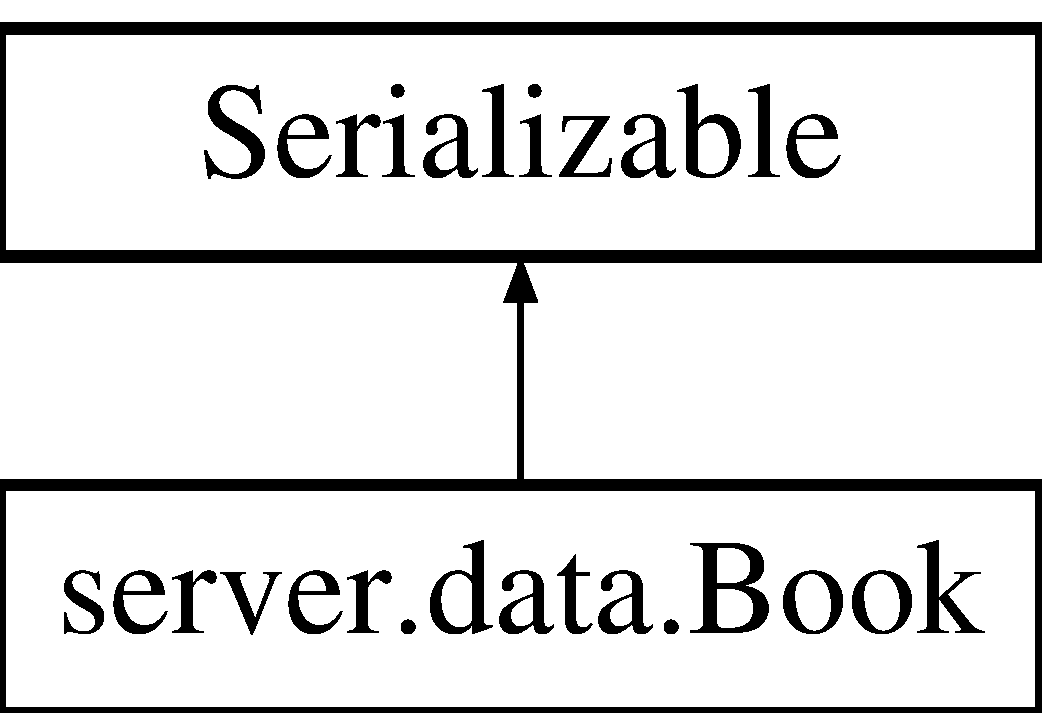
\includegraphics[height=2.000000cm]{classserver_1_1data_1_1_book}
\end{center}
\end{figure}
\subsection*{Public Member Functions}
\begin{DoxyCompactItemize}
\item 
\hyperlink{classserver_1_1data_1_1_book_aa625590266861f80eea48d26f979a483}{Book} (int I\+S\+BN, String title, String category, String edition, String author, double price, String description, String img)
\item 
\hyperlink{classserver_1_1data_1_1_book_a7cfac0c9e49e46d1a04746612ba1cb14}{Book} (int I\+S\+BN, String title, String author, double price)
\item 
void \hyperlink{classserver_1_1data_1_1_book_a8c44fbc3a0d63d0726cb967a3f65203c}{add\+Review} (\hyperlink{classserver_1_1data_1_1_review}{Review} review)
\item 
void \hyperlink{classserver_1_1data_1_1_book_a683834787e9b5010fff13c20b5843b55}{remove\+Review} (\hyperlink{classserver_1_1data_1_1_review}{Review} review)
\item 
List$<$ \hyperlink{classserver_1_1data_1_1_review}{Review} $>$ \hyperlink{classserver_1_1data_1_1_book_ab886271b0fb4f4d4ce3b05967820e118}{get\+Reviews} ()
\item 
void \hyperlink{classserver_1_1data_1_1_book_a0674e14f5b06b73f42fe846c8ad91c9e}{add\+User} (\hyperlink{classserver_1_1data_1_1_user}{User} user)
\item 
void \hyperlink{classserver_1_1data_1_1_book_a6fc896945914513ef9e333c09ef7dd13}{remove\+User} (\hyperlink{classserver_1_1data_1_1_user}{User} user)
\item 
List$<$ \hyperlink{classserver_1_1data_1_1_user}{User} $>$ \hyperlink{classserver_1_1data_1_1_book_a82b3f1dab8f578e8b48e05ca7953f5ae}{get\+Users} ()
\item 
int \hyperlink{classserver_1_1data_1_1_book_ab983c94721d2f5be590871cc0afd1d88}{get\+I\+S\+BN} ()
\item 
void \hyperlink{classserver_1_1data_1_1_book_a70559b3d9b96055ac293d0bb712f18e8}{set\+I\+S\+BN} (int I\+S\+BN)
\item 
String \hyperlink{classserver_1_1data_1_1_book_a74b0812ebfb23009cb65b4f4fda1f828}{get\+Title} ()
\item 
void \hyperlink{classserver_1_1data_1_1_book_aaab2ea46310686520765773057d0f511}{set\+Title} (String title)
\item 
String \hyperlink{classserver_1_1data_1_1_book_a7cc7af6515b25828f2caa978b4a4a720}{get\+Category} ()
\item 
void \hyperlink{classserver_1_1data_1_1_book_afac718f4a0738340cd39fa928672924c}{set\+Category} (String category)
\item 
String \hyperlink{classserver_1_1data_1_1_book_ad5bde468e4e453f38ecbc6deec70dd1f}{get\+Edition} ()
\item 
void \hyperlink{classserver_1_1data_1_1_book_a5b5aff00a34f6810bcd2741d00ac087a}{set\+Edition} (String edition)
\item 
String \hyperlink{classserver_1_1data_1_1_book_ae48ef2e01c143af71e24adcd9580337f}{get\+Author} ()
\item 
void \hyperlink{classserver_1_1data_1_1_book_a7d7e1dbd391d765d6d941e19a61ecae5}{set\+Author} (String author)
\item 
double \hyperlink{classserver_1_1data_1_1_book_aeafc0515d27d8e6d8403f852ab1ff0d0}{get\+Price} ()
\item 
void \hyperlink{classserver_1_1data_1_1_book_a7be7befe21ce4dd863538a0c4682a4db}{set\+Price} (double price)
\item 
String \hyperlink{classserver_1_1data_1_1_book_a4cb323c7591eb56ef4e660b54a972e7f}{get\+Description} ()
\item 
void \hyperlink{classserver_1_1data_1_1_book_abe0edd9bc6fb2f263d6df6873fede27c}{set\+Description} (String description)
\item 
String \hyperlink{classserver_1_1data_1_1_book_af9bd040112c4093a0eb998258e6a318a}{get\+Img} ()
\item 
void \hyperlink{classserver_1_1data_1_1_book_afb3d789fa8cbb8413ccd4189533af83b}{set\+Img} (String img)
\item 
String \hyperlink{classserver_1_1data_1_1_book_ae63b18e3c565ce684821eb4c42f4631c}{to\+String} ()
\end{DoxyCompactItemize}


\subsection{Constructor \& Destructor Documentation}
\mbox{\Hypertarget{classserver_1_1data_1_1_book_aa625590266861f80eea48d26f979a483}\label{classserver_1_1data_1_1_book_aa625590266861f80eea48d26f979a483}} 
\index{server\+::data\+::\+Book@{server\+::data\+::\+Book}!Book@{Book}}
\index{Book@{Book}!server\+::data\+::\+Book@{server\+::data\+::\+Book}}
\subsubsection{\texorpdfstring{Book()}{Book()}\hspace{0.1cm}{\footnotesize\ttfamily [1/2]}}
{\footnotesize\ttfamily server.\+data.\+Book.\+Book (\begin{DoxyParamCaption}\item[{int}]{I\+S\+BN,  }\item[{String}]{title,  }\item[{String}]{category,  }\item[{String}]{edition,  }\item[{String}]{author,  }\item[{double}]{price,  }\item[{String}]{description,  }\item[{String}]{img }\end{DoxyParamCaption})}

\mbox{\Hypertarget{classserver_1_1data_1_1_book_a7cfac0c9e49e46d1a04746612ba1cb14}\label{classserver_1_1data_1_1_book_a7cfac0c9e49e46d1a04746612ba1cb14}} 
\index{server\+::data\+::\+Book@{server\+::data\+::\+Book}!Book@{Book}}
\index{Book@{Book}!server\+::data\+::\+Book@{server\+::data\+::\+Book}}
\subsubsection{\texorpdfstring{Book()}{Book()}\hspace{0.1cm}{\footnotesize\ttfamily [2/2]}}
{\footnotesize\ttfamily server.\+data.\+Book.\+Book (\begin{DoxyParamCaption}\item[{int}]{I\+S\+BN,  }\item[{String}]{title,  }\item[{String}]{author,  }\item[{double}]{price }\end{DoxyParamCaption})}



\subsection{Member Function Documentation}
\mbox{\Hypertarget{classserver_1_1data_1_1_book_a8c44fbc3a0d63d0726cb967a3f65203c}\label{classserver_1_1data_1_1_book_a8c44fbc3a0d63d0726cb967a3f65203c}} 
\index{server\+::data\+::\+Book@{server\+::data\+::\+Book}!add\+Review@{add\+Review}}
\index{add\+Review@{add\+Review}!server\+::data\+::\+Book@{server\+::data\+::\+Book}}
\subsubsection{\texorpdfstring{add\+Review()}{addReview()}}
{\footnotesize\ttfamily void server.\+data.\+Book.\+add\+Review (\begin{DoxyParamCaption}\item[{\hyperlink{classserver_1_1data_1_1_review}{Review}}]{review }\end{DoxyParamCaption})}

\mbox{\Hypertarget{classserver_1_1data_1_1_book_a0674e14f5b06b73f42fe846c8ad91c9e}\label{classserver_1_1data_1_1_book_a0674e14f5b06b73f42fe846c8ad91c9e}} 
\index{server\+::data\+::\+Book@{server\+::data\+::\+Book}!add\+User@{add\+User}}
\index{add\+User@{add\+User}!server\+::data\+::\+Book@{server\+::data\+::\+Book}}
\subsubsection{\texorpdfstring{add\+User()}{addUser()}}
{\footnotesize\ttfamily void server.\+data.\+Book.\+add\+User (\begin{DoxyParamCaption}\item[{\hyperlink{classserver_1_1data_1_1_user}{User}}]{user }\end{DoxyParamCaption})}

\mbox{\Hypertarget{classserver_1_1data_1_1_book_ae48ef2e01c143af71e24adcd9580337f}\label{classserver_1_1data_1_1_book_ae48ef2e01c143af71e24adcd9580337f}} 
\index{server\+::data\+::\+Book@{server\+::data\+::\+Book}!get\+Author@{get\+Author}}
\index{get\+Author@{get\+Author}!server\+::data\+::\+Book@{server\+::data\+::\+Book}}
\subsubsection{\texorpdfstring{get\+Author()}{getAuthor()}}
{\footnotesize\ttfamily String server.\+data.\+Book.\+get\+Author (\begin{DoxyParamCaption}{ }\end{DoxyParamCaption})}

\mbox{\Hypertarget{classserver_1_1data_1_1_book_a7cc7af6515b25828f2caa978b4a4a720}\label{classserver_1_1data_1_1_book_a7cc7af6515b25828f2caa978b4a4a720}} 
\index{server\+::data\+::\+Book@{server\+::data\+::\+Book}!get\+Category@{get\+Category}}
\index{get\+Category@{get\+Category}!server\+::data\+::\+Book@{server\+::data\+::\+Book}}
\subsubsection{\texorpdfstring{get\+Category()}{getCategory()}}
{\footnotesize\ttfamily String server.\+data.\+Book.\+get\+Category (\begin{DoxyParamCaption}{ }\end{DoxyParamCaption})}

\mbox{\Hypertarget{classserver_1_1data_1_1_book_a4cb323c7591eb56ef4e660b54a972e7f}\label{classserver_1_1data_1_1_book_a4cb323c7591eb56ef4e660b54a972e7f}} 
\index{server\+::data\+::\+Book@{server\+::data\+::\+Book}!get\+Description@{get\+Description}}
\index{get\+Description@{get\+Description}!server\+::data\+::\+Book@{server\+::data\+::\+Book}}
\subsubsection{\texorpdfstring{get\+Description()}{getDescription()}}
{\footnotesize\ttfamily String server.\+data.\+Book.\+get\+Description (\begin{DoxyParamCaption}{ }\end{DoxyParamCaption})}

\mbox{\Hypertarget{classserver_1_1data_1_1_book_ad5bde468e4e453f38ecbc6deec70dd1f}\label{classserver_1_1data_1_1_book_ad5bde468e4e453f38ecbc6deec70dd1f}} 
\index{server\+::data\+::\+Book@{server\+::data\+::\+Book}!get\+Edition@{get\+Edition}}
\index{get\+Edition@{get\+Edition}!server\+::data\+::\+Book@{server\+::data\+::\+Book}}
\subsubsection{\texorpdfstring{get\+Edition()}{getEdition()}}
{\footnotesize\ttfamily String server.\+data.\+Book.\+get\+Edition (\begin{DoxyParamCaption}{ }\end{DoxyParamCaption})}

\mbox{\Hypertarget{classserver_1_1data_1_1_book_af9bd040112c4093a0eb998258e6a318a}\label{classserver_1_1data_1_1_book_af9bd040112c4093a0eb998258e6a318a}} 
\index{server\+::data\+::\+Book@{server\+::data\+::\+Book}!get\+Img@{get\+Img}}
\index{get\+Img@{get\+Img}!server\+::data\+::\+Book@{server\+::data\+::\+Book}}
\subsubsection{\texorpdfstring{get\+Img()}{getImg()}}
{\footnotesize\ttfamily String server.\+data.\+Book.\+get\+Img (\begin{DoxyParamCaption}{ }\end{DoxyParamCaption})}

\mbox{\Hypertarget{classserver_1_1data_1_1_book_ab983c94721d2f5be590871cc0afd1d88}\label{classserver_1_1data_1_1_book_ab983c94721d2f5be590871cc0afd1d88}} 
\index{server\+::data\+::\+Book@{server\+::data\+::\+Book}!get\+I\+S\+BN@{get\+I\+S\+BN}}
\index{get\+I\+S\+BN@{get\+I\+S\+BN}!server\+::data\+::\+Book@{server\+::data\+::\+Book}}
\subsubsection{\texorpdfstring{get\+I\+S\+B\+N()}{getISBN()}}
{\footnotesize\ttfamily int server.\+data.\+Book.\+get\+I\+S\+BN (\begin{DoxyParamCaption}{ }\end{DoxyParamCaption})}

\mbox{\Hypertarget{classserver_1_1data_1_1_book_aeafc0515d27d8e6d8403f852ab1ff0d0}\label{classserver_1_1data_1_1_book_aeafc0515d27d8e6d8403f852ab1ff0d0}} 
\index{server\+::data\+::\+Book@{server\+::data\+::\+Book}!get\+Price@{get\+Price}}
\index{get\+Price@{get\+Price}!server\+::data\+::\+Book@{server\+::data\+::\+Book}}
\subsubsection{\texorpdfstring{get\+Price()}{getPrice()}}
{\footnotesize\ttfamily double server.\+data.\+Book.\+get\+Price (\begin{DoxyParamCaption}{ }\end{DoxyParamCaption})}

\mbox{\Hypertarget{classserver_1_1data_1_1_book_ab886271b0fb4f4d4ce3b05967820e118}\label{classserver_1_1data_1_1_book_ab886271b0fb4f4d4ce3b05967820e118}} 
\index{server\+::data\+::\+Book@{server\+::data\+::\+Book}!get\+Reviews@{get\+Reviews}}
\index{get\+Reviews@{get\+Reviews}!server\+::data\+::\+Book@{server\+::data\+::\+Book}}
\subsubsection{\texorpdfstring{get\+Reviews()}{getReviews()}}
{\footnotesize\ttfamily List$<$\hyperlink{classserver_1_1data_1_1_review}{Review}$>$ server.\+data.\+Book.\+get\+Reviews (\begin{DoxyParamCaption}{ }\end{DoxyParamCaption})}

\mbox{\Hypertarget{classserver_1_1data_1_1_book_a74b0812ebfb23009cb65b4f4fda1f828}\label{classserver_1_1data_1_1_book_a74b0812ebfb23009cb65b4f4fda1f828}} 
\index{server\+::data\+::\+Book@{server\+::data\+::\+Book}!get\+Title@{get\+Title}}
\index{get\+Title@{get\+Title}!server\+::data\+::\+Book@{server\+::data\+::\+Book}}
\subsubsection{\texorpdfstring{get\+Title()}{getTitle()}}
{\footnotesize\ttfamily String server.\+data.\+Book.\+get\+Title (\begin{DoxyParamCaption}{ }\end{DoxyParamCaption})}

\mbox{\Hypertarget{classserver_1_1data_1_1_book_a82b3f1dab8f578e8b48e05ca7953f5ae}\label{classserver_1_1data_1_1_book_a82b3f1dab8f578e8b48e05ca7953f5ae}} 
\index{server\+::data\+::\+Book@{server\+::data\+::\+Book}!get\+Users@{get\+Users}}
\index{get\+Users@{get\+Users}!server\+::data\+::\+Book@{server\+::data\+::\+Book}}
\subsubsection{\texorpdfstring{get\+Users()}{getUsers()}}
{\footnotesize\ttfamily List$<$\hyperlink{classserver_1_1data_1_1_user}{User}$>$ server.\+data.\+Book.\+get\+Users (\begin{DoxyParamCaption}{ }\end{DoxyParamCaption})}

\mbox{\Hypertarget{classserver_1_1data_1_1_book_a683834787e9b5010fff13c20b5843b55}\label{classserver_1_1data_1_1_book_a683834787e9b5010fff13c20b5843b55}} 
\index{server\+::data\+::\+Book@{server\+::data\+::\+Book}!remove\+Review@{remove\+Review}}
\index{remove\+Review@{remove\+Review}!server\+::data\+::\+Book@{server\+::data\+::\+Book}}
\subsubsection{\texorpdfstring{remove\+Review()}{removeReview()}}
{\footnotesize\ttfamily void server.\+data.\+Book.\+remove\+Review (\begin{DoxyParamCaption}\item[{\hyperlink{classserver_1_1data_1_1_review}{Review}}]{review }\end{DoxyParamCaption})}

\mbox{\Hypertarget{classserver_1_1data_1_1_book_a6fc896945914513ef9e333c09ef7dd13}\label{classserver_1_1data_1_1_book_a6fc896945914513ef9e333c09ef7dd13}} 
\index{server\+::data\+::\+Book@{server\+::data\+::\+Book}!remove\+User@{remove\+User}}
\index{remove\+User@{remove\+User}!server\+::data\+::\+Book@{server\+::data\+::\+Book}}
\subsubsection{\texorpdfstring{remove\+User()}{removeUser()}}
{\footnotesize\ttfamily void server.\+data.\+Book.\+remove\+User (\begin{DoxyParamCaption}\item[{\hyperlink{classserver_1_1data_1_1_user}{User}}]{user }\end{DoxyParamCaption})}

\mbox{\Hypertarget{classserver_1_1data_1_1_book_a7d7e1dbd391d765d6d941e19a61ecae5}\label{classserver_1_1data_1_1_book_a7d7e1dbd391d765d6d941e19a61ecae5}} 
\index{server\+::data\+::\+Book@{server\+::data\+::\+Book}!set\+Author@{set\+Author}}
\index{set\+Author@{set\+Author}!server\+::data\+::\+Book@{server\+::data\+::\+Book}}
\subsubsection{\texorpdfstring{set\+Author()}{setAuthor()}}
{\footnotesize\ttfamily void server.\+data.\+Book.\+set\+Author (\begin{DoxyParamCaption}\item[{String}]{author }\end{DoxyParamCaption})}

\mbox{\Hypertarget{classserver_1_1data_1_1_book_afac718f4a0738340cd39fa928672924c}\label{classserver_1_1data_1_1_book_afac718f4a0738340cd39fa928672924c}} 
\index{server\+::data\+::\+Book@{server\+::data\+::\+Book}!set\+Category@{set\+Category}}
\index{set\+Category@{set\+Category}!server\+::data\+::\+Book@{server\+::data\+::\+Book}}
\subsubsection{\texorpdfstring{set\+Category()}{setCategory()}}
{\footnotesize\ttfamily void server.\+data.\+Book.\+set\+Category (\begin{DoxyParamCaption}\item[{String}]{category }\end{DoxyParamCaption})}

\mbox{\Hypertarget{classserver_1_1data_1_1_book_abe0edd9bc6fb2f263d6df6873fede27c}\label{classserver_1_1data_1_1_book_abe0edd9bc6fb2f263d6df6873fede27c}} 
\index{server\+::data\+::\+Book@{server\+::data\+::\+Book}!set\+Description@{set\+Description}}
\index{set\+Description@{set\+Description}!server\+::data\+::\+Book@{server\+::data\+::\+Book}}
\subsubsection{\texorpdfstring{set\+Description()}{setDescription()}}
{\footnotesize\ttfamily void server.\+data.\+Book.\+set\+Description (\begin{DoxyParamCaption}\item[{String}]{description }\end{DoxyParamCaption})}

\mbox{\Hypertarget{classserver_1_1data_1_1_book_a5b5aff00a34f6810bcd2741d00ac087a}\label{classserver_1_1data_1_1_book_a5b5aff00a34f6810bcd2741d00ac087a}} 
\index{server\+::data\+::\+Book@{server\+::data\+::\+Book}!set\+Edition@{set\+Edition}}
\index{set\+Edition@{set\+Edition}!server\+::data\+::\+Book@{server\+::data\+::\+Book}}
\subsubsection{\texorpdfstring{set\+Edition()}{setEdition()}}
{\footnotesize\ttfamily void server.\+data.\+Book.\+set\+Edition (\begin{DoxyParamCaption}\item[{String}]{edition }\end{DoxyParamCaption})}

\mbox{\Hypertarget{classserver_1_1data_1_1_book_afb3d789fa8cbb8413ccd4189533af83b}\label{classserver_1_1data_1_1_book_afb3d789fa8cbb8413ccd4189533af83b}} 
\index{server\+::data\+::\+Book@{server\+::data\+::\+Book}!set\+Img@{set\+Img}}
\index{set\+Img@{set\+Img}!server\+::data\+::\+Book@{server\+::data\+::\+Book}}
\subsubsection{\texorpdfstring{set\+Img()}{setImg()}}
{\footnotesize\ttfamily void server.\+data.\+Book.\+set\+Img (\begin{DoxyParamCaption}\item[{String}]{img }\end{DoxyParamCaption})}

\mbox{\Hypertarget{classserver_1_1data_1_1_book_a70559b3d9b96055ac293d0bb712f18e8}\label{classserver_1_1data_1_1_book_a70559b3d9b96055ac293d0bb712f18e8}} 
\index{server\+::data\+::\+Book@{server\+::data\+::\+Book}!set\+I\+S\+BN@{set\+I\+S\+BN}}
\index{set\+I\+S\+BN@{set\+I\+S\+BN}!server\+::data\+::\+Book@{server\+::data\+::\+Book}}
\subsubsection{\texorpdfstring{set\+I\+S\+B\+N()}{setISBN()}}
{\footnotesize\ttfamily void server.\+data.\+Book.\+set\+I\+S\+BN (\begin{DoxyParamCaption}\item[{int}]{I\+S\+BN }\end{DoxyParamCaption})}

\mbox{\Hypertarget{classserver_1_1data_1_1_book_a7be7befe21ce4dd863538a0c4682a4db}\label{classserver_1_1data_1_1_book_a7be7befe21ce4dd863538a0c4682a4db}} 
\index{server\+::data\+::\+Book@{server\+::data\+::\+Book}!set\+Price@{set\+Price}}
\index{set\+Price@{set\+Price}!server\+::data\+::\+Book@{server\+::data\+::\+Book}}
\subsubsection{\texorpdfstring{set\+Price()}{setPrice()}}
{\footnotesize\ttfamily void server.\+data.\+Book.\+set\+Price (\begin{DoxyParamCaption}\item[{double}]{price }\end{DoxyParamCaption})}

\mbox{\Hypertarget{classserver_1_1data_1_1_book_aaab2ea46310686520765773057d0f511}\label{classserver_1_1data_1_1_book_aaab2ea46310686520765773057d0f511}} 
\index{server\+::data\+::\+Book@{server\+::data\+::\+Book}!set\+Title@{set\+Title}}
\index{set\+Title@{set\+Title}!server\+::data\+::\+Book@{server\+::data\+::\+Book}}
\subsubsection{\texorpdfstring{set\+Title()}{setTitle()}}
{\footnotesize\ttfamily void server.\+data.\+Book.\+set\+Title (\begin{DoxyParamCaption}\item[{String}]{title }\end{DoxyParamCaption})}

\mbox{\Hypertarget{classserver_1_1data_1_1_book_ae63b18e3c565ce684821eb4c42f4631c}\label{classserver_1_1data_1_1_book_ae63b18e3c565ce684821eb4c42f4631c}} 
\index{server\+::data\+::\+Book@{server\+::data\+::\+Book}!to\+String@{to\+String}}
\index{to\+String@{to\+String}!server\+::data\+::\+Book@{server\+::data\+::\+Book}}
\subsubsection{\texorpdfstring{to\+String()}{toString()}}
{\footnotesize\ttfamily String server.\+data.\+Book.\+to\+String (\begin{DoxyParamCaption}{ }\end{DoxyParamCaption})}



The documentation for this class was generated from the following file\+:\begin{DoxyCompactItemize}
\item 
src/main/java/server/data/\hyperlink{_book_8java}{Book.\+java}\end{DoxyCompactItemize}

\hypertarget{classclient_1_1_client}{}\section{client.\+Client Class Reference}
\label{classclient_1_1_client}\index{client.\+Client@{client.\+Client}}
\subsection*{Static Public Member Functions}
\begin{DoxyCompactItemize}
\item 
static void \hyperlink{classclient_1_1_client_a54355debc9ffcc61540f7f39241a8a77}{display\+Menu} (String\mbox{[}$\,$\mbox{]} options)
\item 
static void \hyperlink{classclient_1_1_client_a53ffa5e1dd33232694d89f2011acc973}{display\+Sub\+Menu} (String\mbox{[}$\,$\mbox{]} options)
\item 
static void \hyperlink{classclient_1_1_client_abb4f93c11e43c61c21ac7f42a826964c}{main\+Menu} (\hyperlink{interfaceserver_1_1remote_1_1_i_remote}{I\+Remote} server)
\item 
static void \hyperlink{classclient_1_1_client_a5949234ea4d0f331260d4265c8de9967}{menu\+Show\+Books} (\hyperlink{interfaceserver_1_1remote_1_1_i_remote}{I\+Remote} server)
\item 
static void \hyperlink{classclient_1_1_client_aa705054047bb8f7fef9173a9f0980707}{menu\+Search} (\hyperlink{interfaceserver_1_1remote_1_1_i_remote}{I\+Remote} server)
\item 
static void \hyperlink{classclient_1_1_client_aa8fa722000df2208c9a3f4ac7092ea5e}{menu\+Book} (\hyperlink{interfaceserver_1_1remote_1_1_i_remote}{I\+Remote} server)
\item 
static void \hyperlink{classclient_1_1_client_ab5381c77d6c103c49fe3a876e711c318}{menu\+Reviews} (\hyperlink{interfaceserver_1_1remote_1_1_i_remote}{I\+Remote} server)
\item 
static void \hyperlink{classclient_1_1_client_aa9400681614784a26489a925cbdddb0a}{log\+In} (\hyperlink{interfaceserver_1_1remote_1_1_i_remote}{I\+Remote} server)
\item 
static void \hyperlink{classclient_1_1_client_a703b7a8ec73e49a2dafa18c0e99fc2f7}{sign\+Up} (\hyperlink{interfaceserver_1_1remote_1_1_i_remote}{I\+Remote} server)
\item 
static void \hyperlink{classclient_1_1_client_ab4d1b606d620956a59f70c4af4937cc1}{search\+I\+S\+BN} (\hyperlink{interfaceserver_1_1remote_1_1_i_remote}{I\+Remote} server)
\item 
static void \hyperlink{classclient_1_1_client_afb1d6e6867ef984522fd421609af72d0}{search\+Title} (\hyperlink{interfaceserver_1_1remote_1_1_i_remote}{I\+Remote} server)
\item 
static void \hyperlink{classclient_1_1_client_a7ff06b01e82b762056fc7a56e7e58d3d}{show\+Books} (\hyperlink{interfaceserver_1_1remote_1_1_i_remote}{I\+Remote} server)
\item 
static void \hyperlink{classclient_1_1_client_ab3d8c13b4e7328d94819a5300e3c5743}{show\+Book} (\hyperlink{interfaceserver_1_1remote_1_1_i_remote}{I\+Remote} server, int num\+Book)
\item 
static void \hyperlink{classclient_1_1_client_af958ee4c0fed811e49eaa3ee74ae09bf}{buy\+Book} (\hyperlink{interfaceserver_1_1remote_1_1_i_remote}{I\+Remote} server)
\item 
static void \hyperlink{classclient_1_1_client_a535f4e7494d7095589ebf11a8d8f50df}{main} (String\mbox{[}$\,$\mbox{]} args)
\end{DoxyCompactItemize}


\subsection{Member Function Documentation}
\mbox{\Hypertarget{classclient_1_1_client_af958ee4c0fed811e49eaa3ee74ae09bf}\label{classclient_1_1_client_af958ee4c0fed811e49eaa3ee74ae09bf}} 
\index{client\+::\+Client@{client\+::\+Client}!buy\+Book@{buy\+Book}}
\index{buy\+Book@{buy\+Book}!client\+::\+Client@{client\+::\+Client}}
\subsubsection{\texorpdfstring{buy\+Book()}{buyBook()}}
{\footnotesize\ttfamily static void client.\+Client.\+buy\+Book (\begin{DoxyParamCaption}\item[{\hyperlink{interfaceserver_1_1remote_1_1_i_remote}{I\+Remote}}]{server }\end{DoxyParamCaption})\hspace{0.3cm}{\ttfamily [static]}}

\mbox{\Hypertarget{classclient_1_1_client_a54355debc9ffcc61540f7f39241a8a77}\label{classclient_1_1_client_a54355debc9ffcc61540f7f39241a8a77}} 
\index{client\+::\+Client@{client\+::\+Client}!display\+Menu@{display\+Menu}}
\index{display\+Menu@{display\+Menu}!client\+::\+Client@{client\+::\+Client}}
\subsubsection{\texorpdfstring{display\+Menu()}{displayMenu()}}
{\footnotesize\ttfamily static void client.\+Client.\+display\+Menu (\begin{DoxyParamCaption}\item[{String \mbox{[}$\,$\mbox{]}}]{options }\end{DoxyParamCaption})\hspace{0.3cm}{\ttfamily [static]}}

\mbox{\Hypertarget{classclient_1_1_client_a53ffa5e1dd33232694d89f2011acc973}\label{classclient_1_1_client_a53ffa5e1dd33232694d89f2011acc973}} 
\index{client\+::\+Client@{client\+::\+Client}!display\+Sub\+Menu@{display\+Sub\+Menu}}
\index{display\+Sub\+Menu@{display\+Sub\+Menu}!client\+::\+Client@{client\+::\+Client}}
\subsubsection{\texorpdfstring{display\+Sub\+Menu()}{displaySubMenu()}}
{\footnotesize\ttfamily static void client.\+Client.\+display\+Sub\+Menu (\begin{DoxyParamCaption}\item[{String \mbox{[}$\,$\mbox{]}}]{options }\end{DoxyParamCaption})\hspace{0.3cm}{\ttfamily [static]}}

\mbox{\Hypertarget{classclient_1_1_client_aa9400681614784a26489a925cbdddb0a}\label{classclient_1_1_client_aa9400681614784a26489a925cbdddb0a}} 
\index{client\+::\+Client@{client\+::\+Client}!log\+In@{log\+In}}
\index{log\+In@{log\+In}!client\+::\+Client@{client\+::\+Client}}
\subsubsection{\texorpdfstring{log\+In()}{logIn()}}
{\footnotesize\ttfamily static void client.\+Client.\+log\+In (\begin{DoxyParamCaption}\item[{\hyperlink{interfaceserver_1_1remote_1_1_i_remote}{I\+Remote}}]{server }\end{DoxyParamCaption})\hspace{0.3cm}{\ttfamily [static]}}

\mbox{\Hypertarget{classclient_1_1_client_a535f4e7494d7095589ebf11a8d8f50df}\label{classclient_1_1_client_a535f4e7494d7095589ebf11a8d8f50df}} 
\index{client\+::\+Client@{client\+::\+Client}!main@{main}}
\index{main@{main}!client\+::\+Client@{client\+::\+Client}}
\subsubsection{\texorpdfstring{main()}{main()}}
{\footnotesize\ttfamily static void client.\+Client.\+main (\begin{DoxyParamCaption}\item[{String \mbox{[}$\,$\mbox{]}}]{args }\end{DoxyParamCaption})\hspace{0.3cm}{\ttfamily [static]}}

\mbox{\Hypertarget{classclient_1_1_client_abb4f93c11e43c61c21ac7f42a826964c}\label{classclient_1_1_client_abb4f93c11e43c61c21ac7f42a826964c}} 
\index{client\+::\+Client@{client\+::\+Client}!main\+Menu@{main\+Menu}}
\index{main\+Menu@{main\+Menu}!client\+::\+Client@{client\+::\+Client}}
\subsubsection{\texorpdfstring{main\+Menu()}{mainMenu()}}
{\footnotesize\ttfamily static void client.\+Client.\+main\+Menu (\begin{DoxyParamCaption}\item[{\hyperlink{interfaceserver_1_1remote_1_1_i_remote}{I\+Remote}}]{server }\end{DoxyParamCaption})\hspace{0.3cm}{\ttfamily [static]}}

\mbox{\Hypertarget{classclient_1_1_client_aa8fa722000df2208c9a3f4ac7092ea5e}\label{classclient_1_1_client_aa8fa722000df2208c9a3f4ac7092ea5e}} 
\index{client\+::\+Client@{client\+::\+Client}!menu\+Book@{menu\+Book}}
\index{menu\+Book@{menu\+Book}!client\+::\+Client@{client\+::\+Client}}
\subsubsection{\texorpdfstring{menu\+Book()}{menuBook()}}
{\footnotesize\ttfamily static void client.\+Client.\+menu\+Book (\begin{DoxyParamCaption}\item[{\hyperlink{interfaceserver_1_1remote_1_1_i_remote}{I\+Remote}}]{server }\end{DoxyParamCaption})\hspace{0.3cm}{\ttfamily [static]}}

\mbox{\Hypertarget{classclient_1_1_client_ab5381c77d6c103c49fe3a876e711c318}\label{classclient_1_1_client_ab5381c77d6c103c49fe3a876e711c318}} 
\index{client\+::\+Client@{client\+::\+Client}!menu\+Reviews@{menu\+Reviews}}
\index{menu\+Reviews@{menu\+Reviews}!client\+::\+Client@{client\+::\+Client}}
\subsubsection{\texorpdfstring{menu\+Reviews()}{menuReviews()}}
{\footnotesize\ttfamily static void client.\+Client.\+menu\+Reviews (\begin{DoxyParamCaption}\item[{\hyperlink{interfaceserver_1_1remote_1_1_i_remote}{I\+Remote}}]{server }\end{DoxyParamCaption})\hspace{0.3cm}{\ttfamily [static]}}

\mbox{\Hypertarget{classclient_1_1_client_aa705054047bb8f7fef9173a9f0980707}\label{classclient_1_1_client_aa705054047bb8f7fef9173a9f0980707}} 
\index{client\+::\+Client@{client\+::\+Client}!menu\+Search@{menu\+Search}}
\index{menu\+Search@{menu\+Search}!client\+::\+Client@{client\+::\+Client}}
\subsubsection{\texorpdfstring{menu\+Search()}{menuSearch()}}
{\footnotesize\ttfamily static void client.\+Client.\+menu\+Search (\begin{DoxyParamCaption}\item[{\hyperlink{interfaceserver_1_1remote_1_1_i_remote}{I\+Remote}}]{server }\end{DoxyParamCaption})\hspace{0.3cm}{\ttfamily [static]}}

\mbox{\Hypertarget{classclient_1_1_client_a5949234ea4d0f331260d4265c8de9967}\label{classclient_1_1_client_a5949234ea4d0f331260d4265c8de9967}} 
\index{client\+::\+Client@{client\+::\+Client}!menu\+Show\+Books@{menu\+Show\+Books}}
\index{menu\+Show\+Books@{menu\+Show\+Books}!client\+::\+Client@{client\+::\+Client}}
\subsubsection{\texorpdfstring{menu\+Show\+Books()}{menuShowBooks()}}
{\footnotesize\ttfamily static void client.\+Client.\+menu\+Show\+Books (\begin{DoxyParamCaption}\item[{\hyperlink{interfaceserver_1_1remote_1_1_i_remote}{I\+Remote}}]{server }\end{DoxyParamCaption})\hspace{0.3cm}{\ttfamily [static]}}

\mbox{\Hypertarget{classclient_1_1_client_ab4d1b606d620956a59f70c4af4937cc1}\label{classclient_1_1_client_ab4d1b606d620956a59f70c4af4937cc1}} 
\index{client\+::\+Client@{client\+::\+Client}!search\+I\+S\+BN@{search\+I\+S\+BN}}
\index{search\+I\+S\+BN@{search\+I\+S\+BN}!client\+::\+Client@{client\+::\+Client}}
\subsubsection{\texorpdfstring{search\+I\+S\+B\+N()}{searchISBN()}}
{\footnotesize\ttfamily static void client.\+Client.\+search\+I\+S\+BN (\begin{DoxyParamCaption}\item[{\hyperlink{interfaceserver_1_1remote_1_1_i_remote}{I\+Remote}}]{server }\end{DoxyParamCaption})\hspace{0.3cm}{\ttfamily [static]}}

\mbox{\Hypertarget{classclient_1_1_client_afb1d6e6867ef984522fd421609af72d0}\label{classclient_1_1_client_afb1d6e6867ef984522fd421609af72d0}} 
\index{client\+::\+Client@{client\+::\+Client}!search\+Title@{search\+Title}}
\index{search\+Title@{search\+Title}!client\+::\+Client@{client\+::\+Client}}
\subsubsection{\texorpdfstring{search\+Title()}{searchTitle()}}
{\footnotesize\ttfamily static void client.\+Client.\+search\+Title (\begin{DoxyParamCaption}\item[{\hyperlink{interfaceserver_1_1remote_1_1_i_remote}{I\+Remote}}]{server }\end{DoxyParamCaption})\hspace{0.3cm}{\ttfamily [static]}}

\mbox{\Hypertarget{classclient_1_1_client_ab3d8c13b4e7328d94819a5300e3c5743}\label{classclient_1_1_client_ab3d8c13b4e7328d94819a5300e3c5743}} 
\index{client\+::\+Client@{client\+::\+Client}!show\+Book@{show\+Book}}
\index{show\+Book@{show\+Book}!client\+::\+Client@{client\+::\+Client}}
\subsubsection{\texorpdfstring{show\+Book()}{showBook()}}
{\footnotesize\ttfamily static void client.\+Client.\+show\+Book (\begin{DoxyParamCaption}\item[{\hyperlink{interfaceserver_1_1remote_1_1_i_remote}{I\+Remote}}]{server,  }\item[{int}]{num\+Book }\end{DoxyParamCaption})\hspace{0.3cm}{\ttfamily [static]}}

\mbox{\Hypertarget{classclient_1_1_client_a7ff06b01e82b762056fc7a56e7e58d3d}\label{classclient_1_1_client_a7ff06b01e82b762056fc7a56e7e58d3d}} 
\index{client\+::\+Client@{client\+::\+Client}!show\+Books@{show\+Books}}
\index{show\+Books@{show\+Books}!client\+::\+Client@{client\+::\+Client}}
\subsubsection{\texorpdfstring{show\+Books()}{showBooks()}}
{\footnotesize\ttfamily static void client.\+Client.\+show\+Books (\begin{DoxyParamCaption}\item[{\hyperlink{interfaceserver_1_1remote_1_1_i_remote}{I\+Remote}}]{server }\end{DoxyParamCaption})\hspace{0.3cm}{\ttfamily [static]}}

\mbox{\Hypertarget{classclient_1_1_client_a703b7a8ec73e49a2dafa18c0e99fc2f7}\label{classclient_1_1_client_a703b7a8ec73e49a2dafa18c0e99fc2f7}} 
\index{client\+::\+Client@{client\+::\+Client}!sign\+Up@{sign\+Up}}
\index{sign\+Up@{sign\+Up}!client\+::\+Client@{client\+::\+Client}}
\subsubsection{\texorpdfstring{sign\+Up()}{signUp()}}
{\footnotesize\ttfamily static void client.\+Client.\+sign\+Up (\begin{DoxyParamCaption}\item[{\hyperlink{interfaceserver_1_1remote_1_1_i_remote}{I\+Remote}}]{server }\end{DoxyParamCaption})\hspace{0.3cm}{\ttfamily [static]}}



The documentation for this class was generated from the following file\+:\begin{DoxyCompactItemize}
\item 
src/main/java/client/\hyperlink{_client_8java}{Client.\+java}\end{DoxyCompactItemize}

\hypertarget{classserver_1_1_conti_perf_test}{}\section{server.\+Conti\+Perf\+Test Class Reference}
\label{classserver_1_1_conti_perf_test}\index{server.\+Conti\+Perf\+Test@{server.\+Conti\+Perf\+Test}}
\subsection*{Public Member Functions}
\begin{DoxyCompactItemize}
\item 
void \hyperlink{classserver_1_1_conti_perf_test_a4519e539cdbf6975489a13d246a96dac}{store\+Book} ()
\item 
void \hyperlink{classserver_1_1_conti_perf_test_acacbe8ed83af069e2efcf720459e2ea8}{register\+New\+User\+Test} ()
\item 
void \hyperlink{classserver_1_1_conti_perf_test_acc7afc2bd786df7421391f55cba0b6fb}{store\+Book\+Duration} ()
\item 
void \hyperlink{classserver_1_1_conti_perf_test_a8dc9d4ff544289aaa6cfc25f7dfc784f}{show\+Book\+Threads} ()
\item 
void \hyperlink{classserver_1_1_conti_perf_test_aa2bd1869a97663b983e81a1904788e6d}{show\+Book\+Threads2} ()
\end{DoxyCompactItemize}
\subsection*{Static Public Member Functions}
\begin{DoxyCompactItemize}
\item 
static junit.\+framework.\+Test \hyperlink{classserver_1_1_conti_perf_test_a739c19f2d3d32240270589eb76a7e25e}{suite} ()
\end{DoxyCompactItemize}
\subsection*{Public Attributes}
\begin{DoxyCompactItemize}
\item 
Conti\+Perf\+Rule \hyperlink{classserver_1_1_conti_perf_test_a6caa32512d9e7998889ab0126a9a1115}{rule} = new Conti\+Perf\+Rule()
\end{DoxyCompactItemize}


\subsection{Member Function Documentation}
\mbox{\Hypertarget{classserver_1_1_conti_perf_test_acacbe8ed83af069e2efcf720459e2ea8}\label{classserver_1_1_conti_perf_test_acacbe8ed83af069e2efcf720459e2ea8}} 
\index{server\+::\+Conti\+Perf\+Test@{server\+::\+Conti\+Perf\+Test}!register\+New\+User\+Test@{register\+New\+User\+Test}}
\index{register\+New\+User\+Test@{register\+New\+User\+Test}!server\+::\+Conti\+Perf\+Test@{server\+::\+Conti\+Perf\+Test}}
\subsubsection{\texorpdfstring{register\+New\+User\+Test()}{registerNewUserTest()}}
{\footnotesize\ttfamily void server.\+Conti\+Perf\+Test.\+register\+New\+User\+Test (\begin{DoxyParamCaption}{ }\end{DoxyParamCaption})}

\mbox{\Hypertarget{classserver_1_1_conti_perf_test_a8dc9d4ff544289aaa6cfc25f7dfc784f}\label{classserver_1_1_conti_perf_test_a8dc9d4ff544289aaa6cfc25f7dfc784f}} 
\index{server\+::\+Conti\+Perf\+Test@{server\+::\+Conti\+Perf\+Test}!show\+Book\+Threads@{show\+Book\+Threads}}
\index{show\+Book\+Threads@{show\+Book\+Threads}!server\+::\+Conti\+Perf\+Test@{server\+::\+Conti\+Perf\+Test}}
\subsubsection{\texorpdfstring{show\+Book\+Threads()}{showBookThreads()}}
{\footnotesize\ttfamily void server.\+Conti\+Perf\+Test.\+show\+Book\+Threads (\begin{DoxyParamCaption}{ }\end{DoxyParamCaption})}

\mbox{\Hypertarget{classserver_1_1_conti_perf_test_aa2bd1869a97663b983e81a1904788e6d}\label{classserver_1_1_conti_perf_test_aa2bd1869a97663b983e81a1904788e6d}} 
\index{server\+::\+Conti\+Perf\+Test@{server\+::\+Conti\+Perf\+Test}!show\+Book\+Threads2@{show\+Book\+Threads2}}
\index{show\+Book\+Threads2@{show\+Book\+Threads2}!server\+::\+Conti\+Perf\+Test@{server\+::\+Conti\+Perf\+Test}}
\subsubsection{\texorpdfstring{show\+Book\+Threads2()}{showBookThreads2()}}
{\footnotesize\ttfamily void server.\+Conti\+Perf\+Test.\+show\+Book\+Threads2 (\begin{DoxyParamCaption}{ }\end{DoxyParamCaption})}

\mbox{\Hypertarget{classserver_1_1_conti_perf_test_a4519e539cdbf6975489a13d246a96dac}\label{classserver_1_1_conti_perf_test_a4519e539cdbf6975489a13d246a96dac}} 
\index{server\+::\+Conti\+Perf\+Test@{server\+::\+Conti\+Perf\+Test}!store\+Book@{store\+Book}}
\index{store\+Book@{store\+Book}!server\+::\+Conti\+Perf\+Test@{server\+::\+Conti\+Perf\+Test}}
\subsubsection{\texorpdfstring{store\+Book()}{storeBook()}}
{\footnotesize\ttfamily void server.\+Conti\+Perf\+Test.\+store\+Book (\begin{DoxyParamCaption}{ }\end{DoxyParamCaption})}

\mbox{\Hypertarget{classserver_1_1_conti_perf_test_acc7afc2bd786df7421391f55cba0b6fb}\label{classserver_1_1_conti_perf_test_acc7afc2bd786df7421391f55cba0b6fb}} 
\index{server\+::\+Conti\+Perf\+Test@{server\+::\+Conti\+Perf\+Test}!store\+Book\+Duration@{store\+Book\+Duration}}
\index{store\+Book\+Duration@{store\+Book\+Duration}!server\+::\+Conti\+Perf\+Test@{server\+::\+Conti\+Perf\+Test}}
\subsubsection{\texorpdfstring{store\+Book\+Duration()}{storeBookDuration()}}
{\footnotesize\ttfamily void server.\+Conti\+Perf\+Test.\+store\+Book\+Duration (\begin{DoxyParamCaption}{ }\end{DoxyParamCaption})}

\mbox{\Hypertarget{classserver_1_1_conti_perf_test_a739c19f2d3d32240270589eb76a7e25e}\label{classserver_1_1_conti_perf_test_a739c19f2d3d32240270589eb76a7e25e}} 
\index{server\+::\+Conti\+Perf\+Test@{server\+::\+Conti\+Perf\+Test}!suite@{suite}}
\index{suite@{suite}!server\+::\+Conti\+Perf\+Test@{server\+::\+Conti\+Perf\+Test}}
\subsubsection{\texorpdfstring{suite()}{suite()}}
{\footnotesize\ttfamily static junit.\+framework.\+Test server.\+Conti\+Perf\+Test.\+suite (\begin{DoxyParamCaption}{ }\end{DoxyParamCaption})\hspace{0.3cm}{\ttfamily [static]}}



\subsection{Member Data Documentation}
\mbox{\Hypertarget{classserver_1_1_conti_perf_test_a6caa32512d9e7998889ab0126a9a1115}\label{classserver_1_1_conti_perf_test_a6caa32512d9e7998889ab0126a9a1115}} 
\index{server\+::\+Conti\+Perf\+Test@{server\+::\+Conti\+Perf\+Test}!rule@{rule}}
\index{rule@{rule}!server\+::\+Conti\+Perf\+Test@{server\+::\+Conti\+Perf\+Test}}
\subsubsection{\texorpdfstring{rule}{rule}}
{\footnotesize\ttfamily Conti\+Perf\+Rule server.\+Conti\+Perf\+Test.\+rule = new Conti\+Perf\+Rule()}



The documentation for this class was generated from the following file\+:\begin{DoxyCompactItemize}
\item 
src/test/java/server/\hyperlink{_conti_perf_test_8java}{Conti\+Perf\+Test.\+java}\end{DoxyCompactItemize}

\hypertarget{classdb_1_1_d_a_o}{}\section{db.\+D\+AO Class Reference}
\label{classdb_1_1_d_a_o}\index{db.\+D\+AO@{db.\+D\+AO}}
Inheritance diagram for db.\+D\+AO\+:\begin{figure}[H]
\begin{center}
\leavevmode
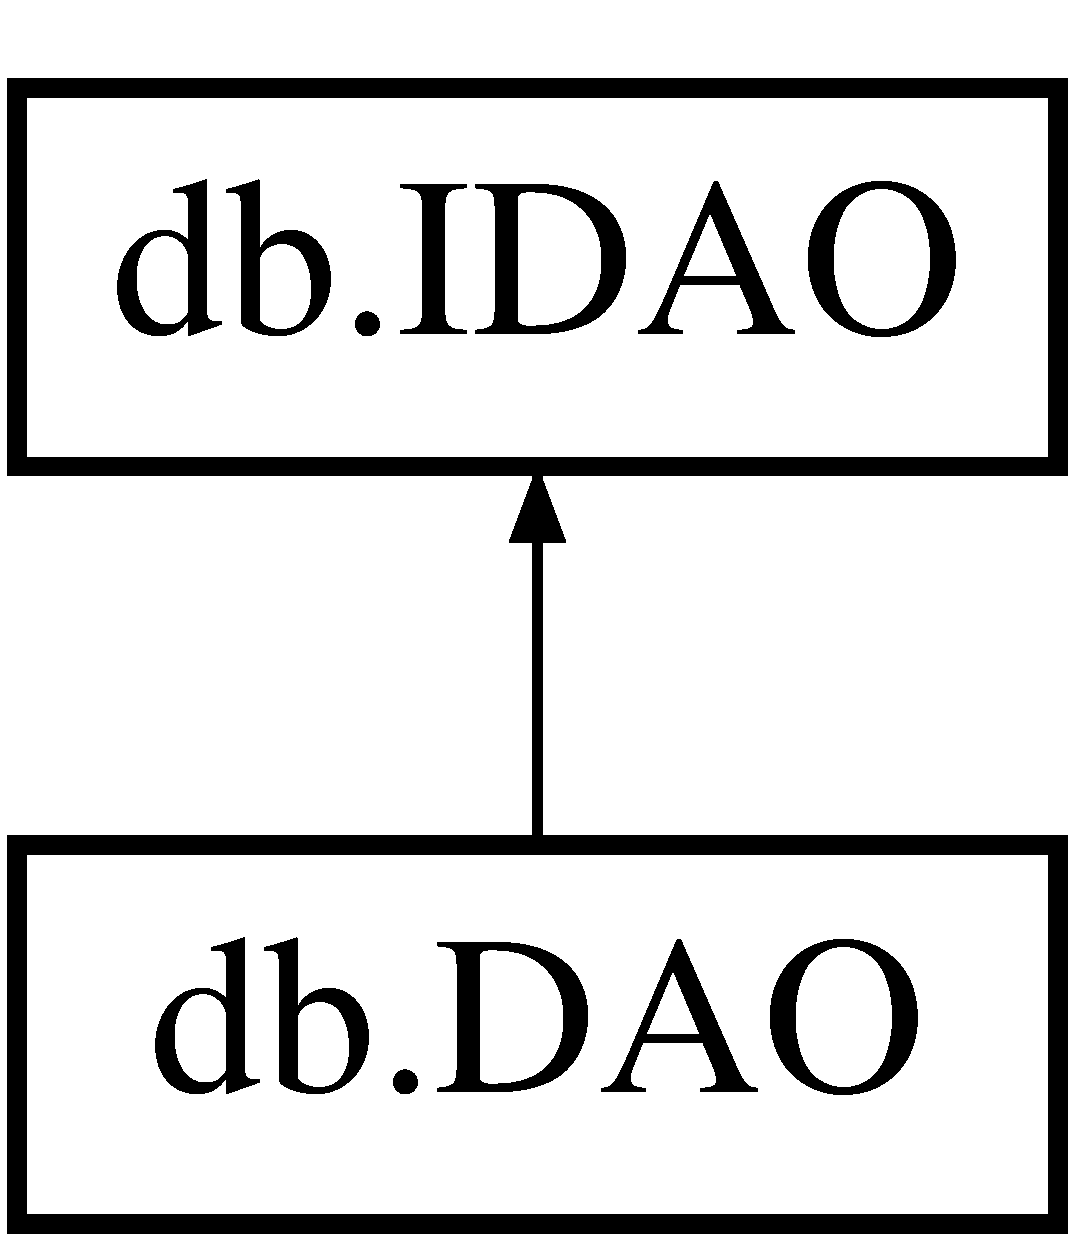
\includegraphics[height=2.000000cm]{classdb_1_1_d_a_o}
\end{center}
\end{figure}
\subsection*{Public Member Functions}
\begin{DoxyCompactItemize}
\item 
\hyperlink{classdb_1_1_d_a_o_abd016ae9834e8d5e94d96f551d1636e7}{D\+AO} ()
\item 
boolean \hyperlink{classdb_1_1_d_a_o_a1600c5d7d28eb225fc7c244fdfb16150}{store\+User} (\hyperlink{classserver_1_1data_1_1_user}{User} u)
\item 
\hyperlink{classserver_1_1data_1_1_user}{User} \hyperlink{classdb_1_1_d_a_o_a6da084ffd9b0da23acba9dc68e747303}{retrieve\+User} (String email)
\item 
boolean \hyperlink{classdb_1_1_d_a_o_a5cd4462deb77065c2d12471cd73b3ec8}{update\+User} (\hyperlink{classserver_1_1data_1_1_user}{User} u)
\item 
\hyperlink{classserver_1_1data_1_1_review}{Review} \hyperlink{classdb_1_1_d_a_o_ae43e182fae8ee7028db6ff17c2d5768f}{retrieve\+Review} (int id\+\_\+review)
\item 
boolean \hyperlink{classdb_1_1_d_a_o_ab73940ac7600902ea7d52bcd041a9c6e}{update\+Review} (\hyperlink{classserver_1_1data_1_1_review}{Review} review)
\item 
boolean \hyperlink{classdb_1_1_d_a_o_a036246b8124d7ac8a36e3eaafd3eb81a}{store\+Book} (\hyperlink{classserver_1_1data_1_1_book}{Book} b)
\item 
\hyperlink{classserver_1_1data_1_1_book}{Book} \hyperlink{classdb_1_1_d_a_o_ade778f907d0a74dc27c4fc03f8709815}{retrieve\+Book} (int I\+S\+BN)
\item 
boolean \hyperlink{classdb_1_1_d_a_o_a4ea10c177ef93a3084ed74b38556adca}{update\+Book} (\hyperlink{classserver_1_1data_1_1_book}{Book} b)
\item 
\hyperlink{classserver_1_1data_1_1_book}{Book} \hyperlink{classdb_1_1_d_a_o_a1f8580da682f8a8af4896c491c3b6611}{retrieve\+Book\+By\+Parameter} (String title)
\item 
List$<$ \hyperlink{classserver_1_1data_1_1_user}{User} $>$ \hyperlink{classdb_1_1_d_a_o_a3b627b7177990799fd02e0c38b8adb70}{get\+All\+Users} ()
\item 
List$<$ \hyperlink{classserver_1_1data_1_1_review}{Review} $>$ \hyperlink{classdb_1_1_d_a_o_a4df79c7d44b050aa55451db2ecf342f6}{get\+All\+Reviews} ()
\item 
List$<$ \hyperlink{classserver_1_1data_1_1_book}{Book} $>$ \hyperlink{classdb_1_1_d_a_o_a82a8c60ccd0de2f70b69bc36d29aeef8}{get\+All\+Books} ()
\item 
void \hyperlink{classdb_1_1_d_a_o_aa033f83155deb72d59492bcb2b8e4d3a}{delete\+Review} (\hyperlink{classserver_1_1data_1_1_review}{Review} r)
\item 
void \hyperlink{classdb_1_1_d_a_o_a65f6a816c5f6dfb07178daf490f56fdc}{delete\+Book} (\hyperlink{classserver_1_1data_1_1_book}{Book} b)
\end{DoxyCompactItemize}


\subsection{Constructor \& Destructor Documentation}
\mbox{\Hypertarget{classdb_1_1_d_a_o_abd016ae9834e8d5e94d96f551d1636e7}\label{classdb_1_1_d_a_o_abd016ae9834e8d5e94d96f551d1636e7}} 
\index{db\+::\+D\+AO@{db\+::\+D\+AO}!D\+AO@{D\+AO}}
\index{D\+AO@{D\+AO}!db\+::\+D\+AO@{db\+::\+D\+AO}}
\subsubsection{\texorpdfstring{D\+A\+O()}{DAO()}}
{\footnotesize\ttfamily db.\+D\+A\+O.\+D\+AO (\begin{DoxyParamCaption}{ }\end{DoxyParamCaption})}



\subsection{Member Function Documentation}
\mbox{\Hypertarget{classdb_1_1_d_a_o_a65f6a816c5f6dfb07178daf490f56fdc}\label{classdb_1_1_d_a_o_a65f6a816c5f6dfb07178daf490f56fdc}} 
\index{db\+::\+D\+AO@{db\+::\+D\+AO}!delete\+Book@{delete\+Book}}
\index{delete\+Book@{delete\+Book}!db\+::\+D\+AO@{db\+::\+D\+AO}}
\subsubsection{\texorpdfstring{delete\+Book()}{deleteBook()}}
{\footnotesize\ttfamily void db.\+D\+A\+O.\+delete\+Book (\begin{DoxyParamCaption}\item[{\hyperlink{classserver_1_1data_1_1_book}{Book}}]{b }\end{DoxyParamCaption})}

Eliminates a book from the database 
\begin{DoxyParams}{Parameters}
{\em b} & the book to eliminate \\
\hline
\end{DoxyParams}


Implements \hyperlink{interfacedb_1_1_i_d_a_o_a1d6c98ea794177d7fd12c4a028ec29c1}{db.\+I\+D\+AO}.

\mbox{\Hypertarget{classdb_1_1_d_a_o_aa033f83155deb72d59492bcb2b8e4d3a}\label{classdb_1_1_d_a_o_aa033f83155deb72d59492bcb2b8e4d3a}} 
\index{db\+::\+D\+AO@{db\+::\+D\+AO}!delete\+Review@{delete\+Review}}
\index{delete\+Review@{delete\+Review}!db\+::\+D\+AO@{db\+::\+D\+AO}}
\subsubsection{\texorpdfstring{delete\+Review()}{deleteReview()}}
{\footnotesize\ttfamily void db.\+D\+A\+O.\+delete\+Review (\begin{DoxyParamCaption}\item[{\hyperlink{classserver_1_1data_1_1_review}{Review}}]{r }\end{DoxyParamCaption})}

Eliminates a Review from the database 
\begin{DoxyParams}{Parameters}
{\em r} & the review to eliminate \\
\hline
\end{DoxyParams}


Implements \hyperlink{interfacedb_1_1_i_d_a_o_a78ca80bc2f2b660edeb9eddd8ca9a4b7}{db.\+I\+D\+AO}.

\mbox{\Hypertarget{classdb_1_1_d_a_o_a82a8c60ccd0de2f70b69bc36d29aeef8}\label{classdb_1_1_d_a_o_a82a8c60ccd0de2f70b69bc36d29aeef8}} 
\index{db\+::\+D\+AO@{db\+::\+D\+AO}!get\+All\+Books@{get\+All\+Books}}
\index{get\+All\+Books@{get\+All\+Books}!db\+::\+D\+AO@{db\+::\+D\+AO}}
\subsubsection{\texorpdfstring{get\+All\+Books()}{getAllBooks()}}
{\footnotesize\ttfamily List$<$\hyperlink{classserver_1_1data_1_1_book}{Book}$>$ db.\+D\+A\+O.\+get\+All\+Books (\begin{DoxyParamCaption}{ }\end{DoxyParamCaption})}

get all the Books of the Database \begin{DoxyReturn}{Returns}
A List$<$\+Book$>$ of all users 
\end{DoxyReturn}


Implements \hyperlink{interfacedb_1_1_i_d_a_o_a75a5ebcd7c3421ae7cccc8e2f3b2d9f9}{db.\+I\+D\+AO}.

\mbox{\Hypertarget{classdb_1_1_d_a_o_a4df79c7d44b050aa55451db2ecf342f6}\label{classdb_1_1_d_a_o_a4df79c7d44b050aa55451db2ecf342f6}} 
\index{db\+::\+D\+AO@{db\+::\+D\+AO}!get\+All\+Reviews@{get\+All\+Reviews}}
\index{get\+All\+Reviews@{get\+All\+Reviews}!db\+::\+D\+AO@{db\+::\+D\+AO}}
\subsubsection{\texorpdfstring{get\+All\+Reviews()}{getAllReviews()}}
{\footnotesize\ttfamily List$<$\hyperlink{classserver_1_1data_1_1_review}{Review}$>$ db.\+D\+A\+O.\+get\+All\+Reviews (\begin{DoxyParamCaption}{ }\end{DoxyParamCaption})}

get all the Reviews of the Database \begin{DoxyReturn}{Returns}
A List$<$\+Review$>$ of all users 
\end{DoxyReturn}


Implements \hyperlink{interfacedb_1_1_i_d_a_o_a3d9625d7e5426aad3c2e70fd0174e5f0}{db.\+I\+D\+AO}.

\mbox{\Hypertarget{classdb_1_1_d_a_o_a3b627b7177990799fd02e0c38b8adb70}\label{classdb_1_1_d_a_o_a3b627b7177990799fd02e0c38b8adb70}} 
\index{db\+::\+D\+AO@{db\+::\+D\+AO}!get\+All\+Users@{get\+All\+Users}}
\index{get\+All\+Users@{get\+All\+Users}!db\+::\+D\+AO@{db\+::\+D\+AO}}
\subsubsection{\texorpdfstring{get\+All\+Users()}{getAllUsers()}}
{\footnotesize\ttfamily List$<$\hyperlink{classserver_1_1data_1_1_user}{User}$>$ db.\+D\+A\+O.\+get\+All\+Users (\begin{DoxyParamCaption}{ }\end{DoxyParamCaption})}

get all the Users of the Database \begin{DoxyReturn}{Returns}
A List$<$\+User$>$ of all users 
\end{DoxyReturn}


Implements \hyperlink{interfacedb_1_1_i_d_a_o_a88b60729d9517ca9aa31b7db7ae07aee}{db.\+I\+D\+AO}.

\mbox{\Hypertarget{classdb_1_1_d_a_o_ade778f907d0a74dc27c4fc03f8709815}\label{classdb_1_1_d_a_o_ade778f907d0a74dc27c4fc03f8709815}} 
\index{db\+::\+D\+AO@{db\+::\+D\+AO}!retrieve\+Book@{retrieve\+Book}}
\index{retrieve\+Book@{retrieve\+Book}!db\+::\+D\+AO@{db\+::\+D\+AO}}
\subsubsection{\texorpdfstring{retrieve\+Book()}{retrieveBook()}}
{\footnotesize\ttfamily \hyperlink{classserver_1_1data_1_1_book}{Book} db.\+D\+A\+O.\+retrieve\+Book (\begin{DoxyParamCaption}\item[{int}]{I\+S\+BN }\end{DoxyParamCaption})}

Get a Book from the database by its I\+S\+BN 
\begin{DoxyParams}{Parameters}
{\em I\+S\+BN} & \\
\hline
\end{DoxyParams}
\begin{DoxyReturn}{Returns}
The Book 
\end{DoxyReturn}


Implements \hyperlink{interfacedb_1_1_i_d_a_o_a1457ecf91799eaacd17cd3259826fc36}{db.\+I\+D\+AO}.

\mbox{\Hypertarget{classdb_1_1_d_a_o_a1f8580da682f8a8af4896c491c3b6611}\label{classdb_1_1_d_a_o_a1f8580da682f8a8af4896c491c3b6611}} 
\index{db\+::\+D\+AO@{db\+::\+D\+AO}!retrieve\+Book\+By\+Parameter@{retrieve\+Book\+By\+Parameter}}
\index{retrieve\+Book\+By\+Parameter@{retrieve\+Book\+By\+Parameter}!db\+::\+D\+AO@{db\+::\+D\+AO}}
\subsubsection{\texorpdfstring{retrieve\+Book\+By\+Parameter()}{retrieveBookByParameter()}}
{\footnotesize\ttfamily \hyperlink{classserver_1_1data_1_1_book}{Book} db.\+D\+A\+O.\+retrieve\+Book\+By\+Parameter (\begin{DoxyParamCaption}\item[{String}]{title }\end{DoxyParamCaption})}

Get a Book from the database by its title 
\begin{DoxyParams}{Parameters}
{\em title} & of the book \\
\hline
\end{DoxyParams}
\begin{DoxyReturn}{Returns}
The book 
\end{DoxyReturn}


Implements \hyperlink{interfacedb_1_1_i_d_a_o_a4c5eda35bfbba1b0a994efe00f99a544}{db.\+I\+D\+AO}.

\mbox{\Hypertarget{classdb_1_1_d_a_o_ae43e182fae8ee7028db6ff17c2d5768f}\label{classdb_1_1_d_a_o_ae43e182fae8ee7028db6ff17c2d5768f}} 
\index{db\+::\+D\+AO@{db\+::\+D\+AO}!retrieve\+Review@{retrieve\+Review}}
\index{retrieve\+Review@{retrieve\+Review}!db\+::\+D\+AO@{db\+::\+D\+AO}}
\subsubsection{\texorpdfstring{retrieve\+Review()}{retrieveReview()}}
{\footnotesize\ttfamily \hyperlink{classserver_1_1data_1_1_review}{Review} db.\+D\+A\+O.\+retrieve\+Review (\begin{DoxyParamCaption}\item[{int}]{id\+\_\+review }\end{DoxyParamCaption})}

Get a Review from the database by its ID 
\begin{DoxyParams}{Parameters}
{\em id\+\_\+review} & \\
\hline
\end{DoxyParams}
\begin{DoxyReturn}{Returns}
The Review 
\end{DoxyReturn}


Implements \hyperlink{interfacedb_1_1_i_d_a_o_a53fd20610d94f7c5f0f713dad7528c26}{db.\+I\+D\+AO}.

\mbox{\Hypertarget{classdb_1_1_d_a_o_a6da084ffd9b0da23acba9dc68e747303}\label{classdb_1_1_d_a_o_a6da084ffd9b0da23acba9dc68e747303}} 
\index{db\+::\+D\+AO@{db\+::\+D\+AO}!retrieve\+User@{retrieve\+User}}
\index{retrieve\+User@{retrieve\+User}!db\+::\+D\+AO@{db\+::\+D\+AO}}
\subsubsection{\texorpdfstring{retrieve\+User()}{retrieveUser()}}
{\footnotesize\ttfamily \hyperlink{classserver_1_1data_1_1_user}{User} db.\+D\+A\+O.\+retrieve\+User (\begin{DoxyParamCaption}\item[{String}]{email }\end{DoxyParamCaption})}

Get a User form the database by its email 
\begin{DoxyParams}{Parameters}
{\em email} & Email of the user you want to get \\
\hline
\end{DoxyParams}
\begin{DoxyReturn}{Returns}
The User 
\end{DoxyReturn}


Implements \hyperlink{interfacedb_1_1_i_d_a_o_ad00bb5255d0badadbf5244799c3b708f}{db.\+I\+D\+AO}.

\mbox{\Hypertarget{classdb_1_1_d_a_o_a036246b8124d7ac8a36e3eaafd3eb81a}\label{classdb_1_1_d_a_o_a036246b8124d7ac8a36e3eaafd3eb81a}} 
\index{db\+::\+D\+AO@{db\+::\+D\+AO}!store\+Book@{store\+Book}}
\index{store\+Book@{store\+Book}!db\+::\+D\+AO@{db\+::\+D\+AO}}
\subsubsection{\texorpdfstring{store\+Book()}{storeBook()}}
{\footnotesize\ttfamily boolean db.\+D\+A\+O.\+store\+Book (\begin{DoxyParamCaption}\item[{\hyperlink{classserver_1_1data_1_1_book}{Book}}]{b }\end{DoxyParamCaption})}

Store a Book in the database 
\begin{DoxyParams}{Parameters}
{\em b} & the Book you want to store \\
\hline
\end{DoxyParams}
\begin{DoxyReturn}{Returns}
true of false to tell if it worked 
\end{DoxyReturn}


Implements \hyperlink{interfacedb_1_1_i_d_a_o_a39851dc1e1f05af40afeb76a5f8be99a}{db.\+I\+D\+AO}.

\mbox{\Hypertarget{classdb_1_1_d_a_o_a1600c5d7d28eb225fc7c244fdfb16150}\label{classdb_1_1_d_a_o_a1600c5d7d28eb225fc7c244fdfb16150}} 
\index{db\+::\+D\+AO@{db\+::\+D\+AO}!store\+User@{store\+User}}
\index{store\+User@{store\+User}!db\+::\+D\+AO@{db\+::\+D\+AO}}
\subsubsection{\texorpdfstring{store\+User()}{storeUser()}}
{\footnotesize\ttfamily boolean db.\+D\+A\+O.\+store\+User (\begin{DoxyParamCaption}\item[{\hyperlink{classserver_1_1data_1_1_user}{User}}]{u }\end{DoxyParamCaption})}

Store a user in the data\+Base 
\begin{DoxyParams}{Parameters}
{\em u} & User you want to store \\
\hline
\end{DoxyParams}
\begin{DoxyReturn}{Returns}
true of false to tell if it worked 
\end{DoxyReturn}


Implements \hyperlink{interfacedb_1_1_i_d_a_o_a5b1f408c9a25305e977e962faa38b026}{db.\+I\+D\+AO}.

\mbox{\Hypertarget{classdb_1_1_d_a_o_a4ea10c177ef93a3084ed74b38556adca}\label{classdb_1_1_d_a_o_a4ea10c177ef93a3084ed74b38556adca}} 
\index{db\+::\+D\+AO@{db\+::\+D\+AO}!update\+Book@{update\+Book}}
\index{update\+Book@{update\+Book}!db\+::\+D\+AO@{db\+::\+D\+AO}}
\subsubsection{\texorpdfstring{update\+Book()}{updateBook()}}
{\footnotesize\ttfamily boolean db.\+D\+A\+O.\+update\+Book (\begin{DoxyParamCaption}\item[{\hyperlink{classserver_1_1data_1_1_book}{Book}}]{b }\end{DoxyParamCaption})}

Updates the row in the database of a given Book 
\begin{DoxyParams}{Parameters}
{\em b} & the book \\
\hline
\end{DoxyParams}
\begin{DoxyReturn}{Returns}
true of false to tell if it worked 
\end{DoxyReturn}


Implements \hyperlink{interfacedb_1_1_i_d_a_o_a202354d7a3e1231687d543e82c15a6f5}{db.\+I\+D\+AO}.

\mbox{\Hypertarget{classdb_1_1_d_a_o_ab73940ac7600902ea7d52bcd041a9c6e}\label{classdb_1_1_d_a_o_ab73940ac7600902ea7d52bcd041a9c6e}} 
\index{db\+::\+D\+AO@{db\+::\+D\+AO}!update\+Review@{update\+Review}}
\index{update\+Review@{update\+Review}!db\+::\+D\+AO@{db\+::\+D\+AO}}
\subsubsection{\texorpdfstring{update\+Review()}{updateReview()}}
{\footnotesize\ttfamily boolean db.\+D\+A\+O.\+update\+Review (\begin{DoxyParamCaption}\item[{\hyperlink{classserver_1_1data_1_1_review}{Review}}]{r }\end{DoxyParamCaption})}

Updates the row in the database of a given Review 
\begin{DoxyParams}{Parameters}
{\em r} & the review to update \\
\hline
\end{DoxyParams}
\begin{DoxyReturn}{Returns}
true of false to tell if it worked 
\end{DoxyReturn}


Implements \hyperlink{interfacedb_1_1_i_d_a_o_a7288e76ee3ce667c0d0d7ecaeef0d94e}{db.\+I\+D\+AO}.

\mbox{\Hypertarget{classdb_1_1_d_a_o_a5cd4462deb77065c2d12471cd73b3ec8}\label{classdb_1_1_d_a_o_a5cd4462deb77065c2d12471cd73b3ec8}} 
\index{db\+::\+D\+AO@{db\+::\+D\+AO}!update\+User@{update\+User}}
\index{update\+User@{update\+User}!db\+::\+D\+AO@{db\+::\+D\+AO}}
\subsubsection{\texorpdfstring{update\+User()}{updateUser()}}
{\footnotesize\ttfamily boolean db.\+D\+A\+O.\+update\+User (\begin{DoxyParamCaption}\item[{\hyperlink{classserver_1_1data_1_1_user}{User}}]{u }\end{DoxyParamCaption})}

Updates the row in the database of a given User 
\begin{DoxyParams}{Parameters}
{\em u} & User you are updating \\
\hline
\end{DoxyParams}
\begin{DoxyReturn}{Returns}
true of false to tell if it worked 
\end{DoxyReturn}


Implements \hyperlink{interfacedb_1_1_i_d_a_o_adbc5f00b7bcdffb6692367a3c9564193}{db.\+I\+D\+AO}.



The documentation for this class was generated from the following file\+:\begin{DoxyCompactItemize}
\item 
src/main/java/db/\hyperlink{_d_a_o_8java}{D\+A\+O.\+java}\end{DoxyCompactItemize}

\hypertarget{classserver_1_1_d_a_o_mock_test}{}\section{server.\+D\+A\+O\+Mock\+Test Class Reference}
\label{classserver_1_1_d_a_o_mock_test}\index{server.\+D\+A\+O\+Mock\+Test@{server.\+D\+A\+O\+Mock\+Test}}
\subsection*{Public Member Functions}
\begin{DoxyCompactItemize}
\item 
void \hyperlink{classserver_1_1_d_a_o_mock_test_a4043bb7c119e734aec6a995cdcace7e2}{set\+Up} ()  throws Exception 
\item 
void \hyperlink{classserver_1_1_d_a_o_mock_test_a25088a79f562d82b1e09deb3c8d62fab}{test\+Register\+User\+Correctly} ()
\item 
void \hyperlink{classserver_1_1_d_a_o_mock_test_acb2d8f72de99513b776086c9cac2e481}{test\+Register\+User\+Already\+Exists} ()
\item 
void \hyperlink{classserver_1_1_d_a_o_mock_test_aa4be8a06f98d4fd2552b4ef073e5c3dc}{test\+Add\+Book\+Valid} ()  throws Remote\+Exception 
\item 
void \hyperlink{classserver_1_1_d_a_o_mock_test_aea6b337ba88d2f58d7ca05e61d7d8aaa}{test\+Add\+Book\+Invalid\+Remote} ()  throws Remote\+Exception 
\end{DoxyCompactItemize}
\subsection*{Static Public Member Functions}
\begin{DoxyCompactItemize}
\item 
static junit.\+framework.\+Test \hyperlink{classserver_1_1_d_a_o_mock_test_a1b414b7605772f324622e605a8f7768f}{suite} ()
\end{DoxyCompactItemize}


\subsection{Member Function Documentation}
\mbox{\Hypertarget{classserver_1_1_d_a_o_mock_test_a4043bb7c119e734aec6a995cdcace7e2}\label{classserver_1_1_d_a_o_mock_test_a4043bb7c119e734aec6a995cdcace7e2}} 
\index{server\+::\+D\+A\+O\+Mock\+Test@{server\+::\+D\+A\+O\+Mock\+Test}!set\+Up@{set\+Up}}
\index{set\+Up@{set\+Up}!server\+::\+D\+A\+O\+Mock\+Test@{server\+::\+D\+A\+O\+Mock\+Test}}
\subsubsection{\texorpdfstring{set\+Up()}{setUp()}}
{\footnotesize\ttfamily void server.\+D\+A\+O\+Mock\+Test.\+set\+Up (\begin{DoxyParamCaption}{ }\end{DoxyParamCaption}) throws Exception}

\mbox{\Hypertarget{classserver_1_1_d_a_o_mock_test_a1b414b7605772f324622e605a8f7768f}\label{classserver_1_1_d_a_o_mock_test_a1b414b7605772f324622e605a8f7768f}} 
\index{server\+::\+D\+A\+O\+Mock\+Test@{server\+::\+D\+A\+O\+Mock\+Test}!suite@{suite}}
\index{suite@{suite}!server\+::\+D\+A\+O\+Mock\+Test@{server\+::\+D\+A\+O\+Mock\+Test}}
\subsubsection{\texorpdfstring{suite()}{suite()}}
{\footnotesize\ttfamily static junit.\+framework.\+Test server.\+D\+A\+O\+Mock\+Test.\+suite (\begin{DoxyParamCaption}{ }\end{DoxyParamCaption})\hspace{0.3cm}{\ttfamily [static]}}

\mbox{\Hypertarget{classserver_1_1_d_a_o_mock_test_aea6b337ba88d2f58d7ca05e61d7d8aaa}\label{classserver_1_1_d_a_o_mock_test_aea6b337ba88d2f58d7ca05e61d7d8aaa}} 
\index{server\+::\+D\+A\+O\+Mock\+Test@{server\+::\+D\+A\+O\+Mock\+Test}!test\+Add\+Book\+Invalid\+Remote@{test\+Add\+Book\+Invalid\+Remote}}
\index{test\+Add\+Book\+Invalid\+Remote@{test\+Add\+Book\+Invalid\+Remote}!server\+::\+D\+A\+O\+Mock\+Test@{server\+::\+D\+A\+O\+Mock\+Test}}
\subsubsection{\texorpdfstring{test\+Add\+Book\+Invalid\+Remote()}{testAddBookInvalidRemote()}}
{\footnotesize\ttfamily void server.\+D\+A\+O\+Mock\+Test.\+test\+Add\+Book\+Invalid\+Remote (\begin{DoxyParamCaption}{ }\end{DoxyParamCaption}) throws Remote\+Exception}

\mbox{\Hypertarget{classserver_1_1_d_a_o_mock_test_aa4be8a06f98d4fd2552b4ef073e5c3dc}\label{classserver_1_1_d_a_o_mock_test_aa4be8a06f98d4fd2552b4ef073e5c3dc}} 
\index{server\+::\+D\+A\+O\+Mock\+Test@{server\+::\+D\+A\+O\+Mock\+Test}!test\+Add\+Book\+Valid@{test\+Add\+Book\+Valid}}
\index{test\+Add\+Book\+Valid@{test\+Add\+Book\+Valid}!server\+::\+D\+A\+O\+Mock\+Test@{server\+::\+D\+A\+O\+Mock\+Test}}
\subsubsection{\texorpdfstring{test\+Add\+Book\+Valid()}{testAddBookValid()}}
{\footnotesize\ttfamily void server.\+D\+A\+O\+Mock\+Test.\+test\+Add\+Book\+Valid (\begin{DoxyParamCaption}{ }\end{DoxyParamCaption}) throws Remote\+Exception}

\mbox{\Hypertarget{classserver_1_1_d_a_o_mock_test_acb2d8f72de99513b776086c9cac2e481}\label{classserver_1_1_d_a_o_mock_test_acb2d8f72de99513b776086c9cac2e481}} 
\index{server\+::\+D\+A\+O\+Mock\+Test@{server\+::\+D\+A\+O\+Mock\+Test}!test\+Register\+User\+Already\+Exists@{test\+Register\+User\+Already\+Exists}}
\index{test\+Register\+User\+Already\+Exists@{test\+Register\+User\+Already\+Exists}!server\+::\+D\+A\+O\+Mock\+Test@{server\+::\+D\+A\+O\+Mock\+Test}}
\subsubsection{\texorpdfstring{test\+Register\+User\+Already\+Exists()}{testRegisterUserAlreadyExists()}}
{\footnotesize\ttfamily void server.\+D\+A\+O\+Mock\+Test.\+test\+Register\+User\+Already\+Exists (\begin{DoxyParamCaption}{ }\end{DoxyParamCaption})}

\mbox{\Hypertarget{classserver_1_1_d_a_o_mock_test_a25088a79f562d82b1e09deb3c8d62fab}\label{classserver_1_1_d_a_o_mock_test_a25088a79f562d82b1e09deb3c8d62fab}} 
\index{server\+::\+D\+A\+O\+Mock\+Test@{server\+::\+D\+A\+O\+Mock\+Test}!test\+Register\+User\+Correctly@{test\+Register\+User\+Correctly}}
\index{test\+Register\+User\+Correctly@{test\+Register\+User\+Correctly}!server\+::\+D\+A\+O\+Mock\+Test@{server\+::\+D\+A\+O\+Mock\+Test}}
\subsubsection{\texorpdfstring{test\+Register\+User\+Correctly()}{testRegisterUserCorrectly()}}
{\footnotesize\ttfamily void server.\+D\+A\+O\+Mock\+Test.\+test\+Register\+User\+Correctly (\begin{DoxyParamCaption}{ }\end{DoxyParamCaption})}



The documentation for this class was generated from the following file\+:\begin{DoxyCompactItemize}
\item 
src/test/java/server/\hyperlink{_d_a_o_mock_test_8java}{D\+A\+O\+Mock\+Test.\+java}\end{DoxyCompactItemize}

\hypertarget{classdb_1_1_d_b}{}\section{db.\+DB Class Reference}
\label{classdb_1_1_d_b}\index{db.\+DB@{db.\+DB}}
Inheritance diagram for db.\+DB\+:\begin{figure}[H]
\begin{center}
\leavevmode
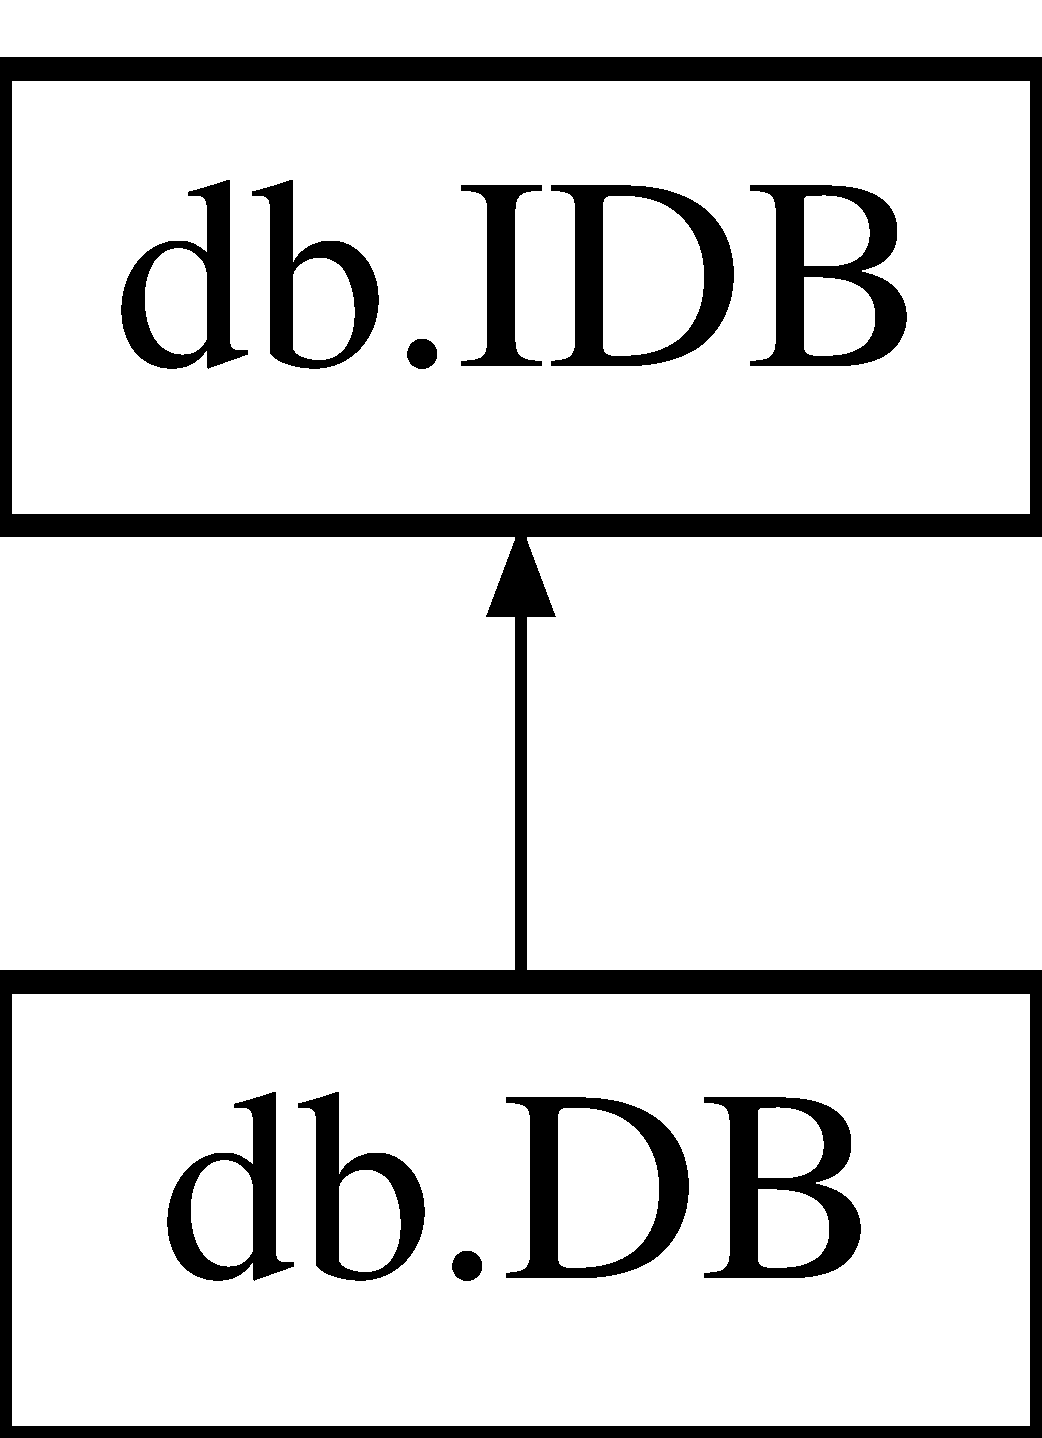
\includegraphics[height=2.000000cm]{classdb_1_1_d_b}
\end{center}
\end{figure}
\subsection*{Public Member Functions}
\begin{DoxyCompactItemize}
\item 
\hyperlink{classdb_1_1_d_b_a1f91d243772e38f908a993724eb01243}{DB} ()
\item 
\hyperlink{classdb_1_1_d_b_afdc419eebbdef14244d859ac59d19dc7}{DB} (\hyperlink{interfacedb_1_1_i_d_a_o}{I\+D\+AO} udao)
\item 
List$<$ \hyperlink{classserver_1_1data_1_1_user}{User} $>$ \hyperlink{classdb_1_1_d_b_ad02e4c78f9afe64af34fb2e5889ce501}{get\+All\+Users} ()
\item 
List$<$ \hyperlink{classserver_1_1data_1_1_review}{Review} $>$ \hyperlink{classdb_1_1_d_b_ac7a84c5621f4ad2263cd830dbf10842e}{get\+All\+Reviews} ()
\item 
List$<$ \hyperlink{classserver_1_1data_1_1_book}{Book} $>$ \hyperlink{classdb_1_1_d_b_ab4fbfd3716967ce37cc462ca04c68ca8}{get\+All\+Books} ()
\item 
boolean \hyperlink{classdb_1_1_d_b_a8a1a15bae4352c3c73092d801ef26c41}{buy\+Book} (String email, String book\+\_\+title)
\item 
boolean \hyperlink{classdb_1_1_d_b_accfa7c2f48252f167576221dc14ff721}{add\+Review} (\hyperlink{classserver_1_1data_1_1_book}{Book} b, \hyperlink{classserver_1_1data_1_1_review}{Review} r, \hyperlink{classserver_1_1data_1_1_user}{User} u)
\item 
boolean \hyperlink{classdb_1_1_d_b_a76fac3ed38eaecd5a073224d6ad51332}{register\+User} (String email, String password, boolean role)
\item 
boolean \hyperlink{classdb_1_1_d_b_aa767c59cde3ca8f76c3acbd0c5348608}{register\+User} (\hyperlink{classserver_1_1data_1_1_user}{User} u)
\item 
boolean \hyperlink{classdb_1_1_d_b_a705ed9c0ffae567ec3ac09fbd7138c6f}{add\+Book\+To\+Db} (\hyperlink{classserver_1_1data_1_1_book}{Book} b)
\item 
\hyperlink{classserver_1_1data_1_1_book}{Book} \hyperlink{classdb_1_1_d_b_ae902ce95ca7433f1f7f77419f4121f4c}{show\+Book\+By\+I\+S\+BN} (int I\+S\+BN)
\item 
\hyperlink{classserver_1_1data_1_1_book}{Book} \hyperlink{classdb_1_1_d_b_a22a4c5b98facd4506b03828697220773}{show\+Book\+By\+Title} (String title)
\item 
\hyperlink{classserver_1_1data_1_1_review}{Review} \hyperlink{classdb_1_1_d_b_a84b36a9e2c155b1aa2868844cd157df7}{show\+Review} (int id\+\_\+review)
\item 
\hyperlink{classserver_1_1data_1_1_user}{User} \hyperlink{classdb_1_1_d_b_a914986669ac622ef33ae344baaefa32c}{show\+User} (String email)
\item 
List$<$ \hyperlink{classserver_1_1data_1_1_review}{Review} $>$ \hyperlink{classdb_1_1_d_b_a9ef4c302b91da17852f09a27a90fb4b5}{get\+User\+Reviews} (String email)
\item 
List$<$ \hyperlink{classserver_1_1data_1_1_review}{Review} $>$ \hyperlink{classdb_1_1_d_b_a02a42ee97d8e7189733dfc720a05452e}{get\+Book\+Reviews} (String title)
\item 
double \hyperlink{classdb_1_1_d_b_a8b2b9d6c4aabb17719e2d2af4cf7ba74}{average\+Rating\+By\+Book} (String title)
\item 
double \hyperlink{classdb_1_1_d_b_a38091677ae1e964a84320d6e539ea62e}{average\+Rating\+By\+User} (String email)
\item 
boolean \hyperlink{classdb_1_1_d_b_ab3664756678e77a9f1b9c6c93c81d691}{delete\+Review} (int id\+\_\+review)
\item 
boolean \hyperlink{classdb_1_1_d_b_a712d418878efa15112c62eb6db4b022d}{delete\+Book} (int I\+S\+BN)
\end{DoxyCompactItemize}


\subsection{Constructor \& Destructor Documentation}
\mbox{\Hypertarget{classdb_1_1_d_b_a1f91d243772e38f908a993724eb01243}\label{classdb_1_1_d_b_a1f91d243772e38f908a993724eb01243}} 
\index{db\+::\+DB@{db\+::\+DB}!DB@{DB}}
\index{DB@{DB}!db\+::\+DB@{db\+::\+DB}}
\subsubsection{\texorpdfstring{D\+B()}{DB()}\hspace{0.1cm}{\footnotesize\ttfamily [1/2]}}
{\footnotesize\ttfamily db.\+D\+B.\+DB (\begin{DoxyParamCaption}{ }\end{DoxyParamCaption})}

\mbox{\Hypertarget{classdb_1_1_d_b_afdc419eebbdef14244d859ac59d19dc7}\label{classdb_1_1_d_b_afdc419eebbdef14244d859ac59d19dc7}} 
\index{db\+::\+DB@{db\+::\+DB}!DB@{DB}}
\index{DB@{DB}!db\+::\+DB@{db\+::\+DB}}
\subsubsection{\texorpdfstring{D\+B()}{DB()}\hspace{0.1cm}{\footnotesize\ttfamily [2/2]}}
{\footnotesize\ttfamily db.\+D\+B.\+DB (\begin{DoxyParamCaption}\item[{\hyperlink{interfacedb_1_1_i_d_a_o}{I\+D\+AO}}]{udao }\end{DoxyParamCaption})}



\subsection{Member Function Documentation}
\mbox{\Hypertarget{classdb_1_1_d_b_a705ed9c0ffae567ec3ac09fbd7138c6f}\label{classdb_1_1_d_b_a705ed9c0ffae567ec3ac09fbd7138c6f}} 
\index{db\+::\+DB@{db\+::\+DB}!add\+Book\+To\+Db@{add\+Book\+To\+Db}}
\index{add\+Book\+To\+Db@{add\+Book\+To\+Db}!db\+::\+DB@{db\+::\+DB}}
\subsubsection{\texorpdfstring{add\+Book\+To\+Db()}{addBookToDb()}}
{\footnotesize\ttfamily boolean db.\+D\+B.\+add\+Book\+To\+Db (\begin{DoxyParamCaption}\item[{\hyperlink{classserver_1_1data_1_1_book}{Book}}]{b }\end{DoxyParamCaption})}

Adds a new book to the database 
\begin{DoxyParams}{Parameters}
{\em b} & the book to add \\
\hline
\end{DoxyParams}
\begin{DoxyReturn}{Returns}
true or false to tell if it worked 
\end{DoxyReturn}


Implements \hyperlink{interfacedb_1_1_i_d_b_a63904b26597f651ea6acbd03384e0afb}{db.\+I\+DB}.

\mbox{\Hypertarget{classdb_1_1_d_b_accfa7c2f48252f167576221dc14ff721}\label{classdb_1_1_d_b_accfa7c2f48252f167576221dc14ff721}} 
\index{db\+::\+DB@{db\+::\+DB}!add\+Review@{add\+Review}}
\index{add\+Review@{add\+Review}!db\+::\+DB@{db\+::\+DB}}
\subsubsection{\texorpdfstring{add\+Review()}{addReview()}}
{\footnotesize\ttfamily boolean db.\+D\+B.\+add\+Review (\begin{DoxyParamCaption}\item[{\hyperlink{classserver_1_1data_1_1_book}{Book}}]{b,  }\item[{\hyperlink{classserver_1_1data_1_1_review}{Review}}]{r,  }\item[{\hyperlink{classserver_1_1data_1_1_user}{User}}]{user }\end{DoxyParamCaption})}

Adds a new Review to the database 
\begin{DoxyParams}{Parameters}
{\em b} & the book its from \\
\hline
{\em r} & the review \\
\hline
{\em user} & the user that wrote it \\
\hline
\end{DoxyParams}
\begin{DoxyReturn}{Returns}
true or false to tell if it worked 
\end{DoxyReturn}


Implements \hyperlink{interfacedb_1_1_i_d_b_a00a453c6d4fc604615f5a173d86600fc}{db.\+I\+DB}.

\mbox{\Hypertarget{classdb_1_1_d_b_a8b2b9d6c4aabb17719e2d2af4cf7ba74}\label{classdb_1_1_d_b_a8b2b9d6c4aabb17719e2d2af4cf7ba74}} 
\index{db\+::\+DB@{db\+::\+DB}!average\+Rating\+By\+Book@{average\+Rating\+By\+Book}}
\index{average\+Rating\+By\+Book@{average\+Rating\+By\+Book}!db\+::\+DB@{db\+::\+DB}}
\subsubsection{\texorpdfstring{average\+Rating\+By\+Book()}{averageRatingByBook()}}
{\footnotesize\ttfamily double db.\+D\+B.\+average\+Rating\+By\+Book (\begin{DoxyParamCaption}\item[{String}]{title }\end{DoxyParamCaption})}

Gets the average rating of a book 
\begin{DoxyParams}{Parameters}
{\em title} & of the book \\
\hline
\end{DoxyParams}
\begin{DoxyReturn}{Returns}
a double the average rating 
\end{DoxyReturn}


Implements \hyperlink{interfacedb_1_1_i_d_b_a4d23da2e383e7fe0638089fb2686b6c3}{db.\+I\+DB}.

\mbox{\Hypertarget{classdb_1_1_d_b_a38091677ae1e964a84320d6e539ea62e}\label{classdb_1_1_d_b_a38091677ae1e964a84320d6e539ea62e}} 
\index{db\+::\+DB@{db\+::\+DB}!average\+Rating\+By\+User@{average\+Rating\+By\+User}}
\index{average\+Rating\+By\+User@{average\+Rating\+By\+User}!db\+::\+DB@{db\+::\+DB}}
\subsubsection{\texorpdfstring{average\+Rating\+By\+User()}{averageRatingByUser()}}
{\footnotesize\ttfamily double db.\+D\+B.\+average\+Rating\+By\+User (\begin{DoxyParamCaption}\item[{String}]{email }\end{DoxyParamCaption})}

Gets the average rating given by a user 
\begin{DoxyParams}{Parameters}
{\em email} & of the user \\
\hline
\end{DoxyParams}
\begin{DoxyReturn}{Returns}
a double the average rating 
\end{DoxyReturn}


Implements \hyperlink{interfacedb_1_1_i_d_b_a5bb2209c976ab0a7f20606ed5df0e0cf}{db.\+I\+DB}.

\mbox{\Hypertarget{classdb_1_1_d_b_a8a1a15bae4352c3c73092d801ef26c41}\label{classdb_1_1_d_b_a8a1a15bae4352c3c73092d801ef26c41}} 
\index{db\+::\+DB@{db\+::\+DB}!buy\+Book@{buy\+Book}}
\index{buy\+Book@{buy\+Book}!db\+::\+DB@{db\+::\+DB}}
\subsubsection{\texorpdfstring{buy\+Book()}{buyBook()}}
{\footnotesize\ttfamily boolean db.\+D\+B.\+buy\+Book (\begin{DoxyParamCaption}\item[{String}]{email,  }\item[{String}]{book\+\_\+title }\end{DoxyParamCaption})}

Allow the User to buy a selected book 
\begin{DoxyParams}{Parameters}
{\em email} & Email of the buying user \\
\hline
{\em book\+\_\+title} & the title of the book to buy \\
\hline
\end{DoxyParams}
\begin{DoxyReturn}{Returns}
true or false to tell if it worked 
\end{DoxyReturn}


Implements \hyperlink{interfacedb_1_1_i_d_b_a2ac985a90e8369fab676950b3fb4c2bc}{db.\+I\+DB}.

\mbox{\Hypertarget{classdb_1_1_d_b_a712d418878efa15112c62eb6db4b022d}\label{classdb_1_1_d_b_a712d418878efa15112c62eb6db4b022d}} 
\index{db\+::\+DB@{db\+::\+DB}!delete\+Book@{delete\+Book}}
\index{delete\+Book@{delete\+Book}!db\+::\+DB@{db\+::\+DB}}
\subsubsection{\texorpdfstring{delete\+Book()}{deleteBook()}}
{\footnotesize\ttfamily boolean db.\+D\+B.\+delete\+Book (\begin{DoxyParamCaption}\item[{int}]{I\+S\+BN }\end{DoxyParamCaption})}

Eliminates a book from the database 
\begin{DoxyParams}{Parameters}
{\em I\+S\+BN} & \\
\hline
\end{DoxyParams}
\begin{DoxyReturn}{Returns}
true or false to tell if it worked 
\end{DoxyReturn}


Implements \hyperlink{interfacedb_1_1_i_d_b_a8fa065455c75f33b9713b8d5058a0e30}{db.\+I\+DB}.

\mbox{\Hypertarget{classdb_1_1_d_b_ab3664756678e77a9f1b9c6c93c81d691}\label{classdb_1_1_d_b_ab3664756678e77a9f1b9c6c93c81d691}} 
\index{db\+::\+DB@{db\+::\+DB}!delete\+Review@{delete\+Review}}
\index{delete\+Review@{delete\+Review}!db\+::\+DB@{db\+::\+DB}}
\subsubsection{\texorpdfstring{delete\+Review()}{deleteReview()}}
{\footnotesize\ttfamily boolean db.\+D\+B.\+delete\+Review (\begin{DoxyParamCaption}\item[{int}]{id\+\_\+review }\end{DoxyParamCaption})}

Eliminates a Review from the database 
\begin{DoxyParams}{Parameters}
{\em id\+\_\+review} & \\
\hline
\end{DoxyParams}
\begin{DoxyReturn}{Returns}
true or false to tell if it worked 
\end{DoxyReturn}


Implements \hyperlink{interfacedb_1_1_i_d_b_a37810242fa48895f21f790ef6a367225}{db.\+I\+DB}.

\mbox{\Hypertarget{classdb_1_1_d_b_ab4fbfd3716967ce37cc462ca04c68ca8}\label{classdb_1_1_d_b_ab4fbfd3716967ce37cc462ca04c68ca8}} 
\index{db\+::\+DB@{db\+::\+DB}!get\+All\+Books@{get\+All\+Books}}
\index{get\+All\+Books@{get\+All\+Books}!db\+::\+DB@{db\+::\+DB}}
\subsubsection{\texorpdfstring{get\+All\+Books()}{getAllBooks()}}
{\footnotesize\ttfamily List$<$\hyperlink{classserver_1_1data_1_1_book}{Book}$>$ db.\+D\+B.\+get\+All\+Books (\begin{DoxyParamCaption}{ }\end{DoxyParamCaption})}

get all the Books of the Database \begin{DoxyReturn}{Returns}
A List$<$\+Book$>$ of all users 
\end{DoxyReturn}


Implements \hyperlink{interfacedb_1_1_i_d_b_abd0d41674bbcdd524a3ca2403504bf25}{db.\+I\+DB}.

\mbox{\Hypertarget{classdb_1_1_d_b_ac7a84c5621f4ad2263cd830dbf10842e}\label{classdb_1_1_d_b_ac7a84c5621f4ad2263cd830dbf10842e}} 
\index{db\+::\+DB@{db\+::\+DB}!get\+All\+Reviews@{get\+All\+Reviews}}
\index{get\+All\+Reviews@{get\+All\+Reviews}!db\+::\+DB@{db\+::\+DB}}
\subsubsection{\texorpdfstring{get\+All\+Reviews()}{getAllReviews()}}
{\footnotesize\ttfamily List$<$\hyperlink{classserver_1_1data_1_1_review}{Review}$>$ db.\+D\+B.\+get\+All\+Reviews (\begin{DoxyParamCaption}{ }\end{DoxyParamCaption})}

get all the Reviews of the Database \begin{DoxyReturn}{Returns}
A List$<$\+Review$>$ of all users 
\end{DoxyReturn}


Implements \hyperlink{interfacedb_1_1_i_d_b_a08f60c8b923599c650f04b4192d00d55}{db.\+I\+DB}.

\mbox{\Hypertarget{classdb_1_1_d_b_ad02e4c78f9afe64af34fb2e5889ce501}\label{classdb_1_1_d_b_ad02e4c78f9afe64af34fb2e5889ce501}} 
\index{db\+::\+DB@{db\+::\+DB}!get\+All\+Users@{get\+All\+Users}}
\index{get\+All\+Users@{get\+All\+Users}!db\+::\+DB@{db\+::\+DB}}
\subsubsection{\texorpdfstring{get\+All\+Users()}{getAllUsers()}}
{\footnotesize\ttfamily List$<$\hyperlink{classserver_1_1data_1_1_user}{User}$>$ db.\+D\+B.\+get\+All\+Users (\begin{DoxyParamCaption}{ }\end{DoxyParamCaption})}

get all the Users of the Database \begin{DoxyReturn}{Returns}
A List$<$\+User$>$ of all users 
\end{DoxyReturn}


Implements \hyperlink{interfacedb_1_1_i_d_b_a39ad15619eae3d0ec652e1849e3ebd50}{db.\+I\+DB}.

\mbox{\Hypertarget{classdb_1_1_d_b_a02a42ee97d8e7189733dfc720a05452e}\label{classdb_1_1_d_b_a02a42ee97d8e7189733dfc720a05452e}} 
\index{db\+::\+DB@{db\+::\+DB}!get\+Book\+Reviews@{get\+Book\+Reviews}}
\index{get\+Book\+Reviews@{get\+Book\+Reviews}!db\+::\+DB@{db\+::\+DB}}
\subsubsection{\texorpdfstring{get\+Book\+Reviews()}{getBookReviews()}}
{\footnotesize\ttfamily List$<$\hyperlink{classserver_1_1data_1_1_review}{Review}$>$ db.\+D\+B.\+get\+Book\+Reviews (\begin{DoxyParamCaption}\item[{String}]{title }\end{DoxyParamCaption})}

Get all the reviews of a book 
\begin{DoxyParams}{Parameters}
{\em title} & of the book \\
\hline
\end{DoxyParams}
\begin{DoxyReturn}{Returns}
A List$<$\+Review$>$ of a given book 
\end{DoxyReturn}


Implements \hyperlink{interfacedb_1_1_i_d_b_a6b8fda48df77b542b8713bc4f035bccf}{db.\+I\+DB}.

\mbox{\Hypertarget{classdb_1_1_d_b_a9ef4c302b91da17852f09a27a90fb4b5}\label{classdb_1_1_d_b_a9ef4c302b91da17852f09a27a90fb4b5}} 
\index{db\+::\+DB@{db\+::\+DB}!get\+User\+Reviews@{get\+User\+Reviews}}
\index{get\+User\+Reviews@{get\+User\+Reviews}!db\+::\+DB@{db\+::\+DB}}
\subsubsection{\texorpdfstring{get\+User\+Reviews()}{getUserReviews()}}
{\footnotesize\ttfamily List$<$\hyperlink{classserver_1_1data_1_1_review}{Review}$>$ db.\+D\+B.\+get\+User\+Reviews (\begin{DoxyParamCaption}\item[{String}]{email }\end{DoxyParamCaption})}

Get all the reviews a User wrote 
\begin{DoxyParams}{Parameters}
{\em email} & of the user \\
\hline
\end{DoxyParams}
\begin{DoxyReturn}{Returns}
A List$<$\+Review$>$ of a given user 
\end{DoxyReturn}


Implements \hyperlink{interfacedb_1_1_i_d_b_afd7ee8924344c13a64a1363d1a295771}{db.\+I\+DB}.

\mbox{\Hypertarget{classdb_1_1_d_b_a76fac3ed38eaecd5a073224d6ad51332}\label{classdb_1_1_d_b_a76fac3ed38eaecd5a073224d6ad51332}} 
\index{db\+::\+DB@{db\+::\+DB}!register\+User@{register\+User}}
\index{register\+User@{register\+User}!db\+::\+DB@{db\+::\+DB}}
\subsubsection{\texorpdfstring{register\+User()}{registerUser()}\hspace{0.1cm}{\footnotesize\ttfamily [1/2]}}
{\footnotesize\ttfamily boolean db.\+D\+B.\+register\+User (\begin{DoxyParamCaption}\item[{String}]{email,  }\item[{String}]{password,  }\item[{boolean}]{role }\end{DoxyParamCaption})}

creates a new user 
\begin{DoxyParams}{Parameters}
{\em email} & \\
\hline
{\em password} & \\
\hline
{\em role} & (true admin; false user) \\
\hline
\end{DoxyParams}
\begin{DoxyReturn}{Returns}
true or false to tell if it worked 
\end{DoxyReturn}


Implements \hyperlink{interfacedb_1_1_i_d_b_a92913d9357ef22978adc35d3fb9d3590}{db.\+I\+DB}.

\mbox{\Hypertarget{classdb_1_1_d_b_aa767c59cde3ca8f76c3acbd0c5348608}\label{classdb_1_1_d_b_aa767c59cde3ca8f76c3acbd0c5348608}} 
\index{db\+::\+DB@{db\+::\+DB}!register\+User@{register\+User}}
\index{register\+User@{register\+User}!db\+::\+DB@{db\+::\+DB}}
\subsubsection{\texorpdfstring{register\+User()}{registerUser()}\hspace{0.1cm}{\footnotesize\ttfamily [2/2]}}
{\footnotesize\ttfamily boolean db.\+D\+B.\+register\+User (\begin{DoxyParamCaption}\item[{\hyperlink{classserver_1_1data_1_1_user}{User}}]{u }\end{DoxyParamCaption})}

\mbox{\Hypertarget{classdb_1_1_d_b_ae902ce95ca7433f1f7f77419f4121f4c}\label{classdb_1_1_d_b_ae902ce95ca7433f1f7f77419f4121f4c}} 
\index{db\+::\+DB@{db\+::\+DB}!show\+Book\+By\+I\+S\+BN@{show\+Book\+By\+I\+S\+BN}}
\index{show\+Book\+By\+I\+S\+BN@{show\+Book\+By\+I\+S\+BN}!db\+::\+DB@{db\+::\+DB}}
\subsubsection{\texorpdfstring{show\+Book\+By\+I\+S\+B\+N()}{showBookByISBN()}}
{\footnotesize\ttfamily \hyperlink{classserver_1_1data_1_1_book}{Book} db.\+D\+B.\+show\+Book\+By\+I\+S\+BN (\begin{DoxyParamCaption}\item[{int}]{I\+S\+BN }\end{DoxyParamCaption})}

Get a book from the database by its I\+S\+BN 
\begin{DoxyParams}{Parameters}
{\em I\+S\+BN} & \\
\hline
\end{DoxyParams}
\begin{DoxyReturn}{Returns}
The Book 
\end{DoxyReturn}


Implements \hyperlink{interfacedb_1_1_i_d_b_aed305f6c36ff140084636a8eded479db}{db.\+I\+DB}.

\mbox{\Hypertarget{classdb_1_1_d_b_a22a4c5b98facd4506b03828697220773}\label{classdb_1_1_d_b_a22a4c5b98facd4506b03828697220773}} 
\index{db\+::\+DB@{db\+::\+DB}!show\+Book\+By\+Title@{show\+Book\+By\+Title}}
\index{show\+Book\+By\+Title@{show\+Book\+By\+Title}!db\+::\+DB@{db\+::\+DB}}
\subsubsection{\texorpdfstring{show\+Book\+By\+Title()}{showBookByTitle()}}
{\footnotesize\ttfamily \hyperlink{classserver_1_1data_1_1_book}{Book} db.\+D\+B.\+show\+Book\+By\+Title (\begin{DoxyParamCaption}\item[{String}]{title }\end{DoxyParamCaption})}

Get a Book from the database by its title 
\begin{DoxyParams}{Parameters}
{\em title} & of the book \\
\hline
\end{DoxyParams}
\begin{DoxyReturn}{Returns}
The book 
\end{DoxyReturn}


Implements \hyperlink{interfacedb_1_1_i_d_b_a6418edaf7c25f99f0422c0000db521fa}{db.\+I\+DB}.

\mbox{\Hypertarget{classdb_1_1_d_b_a84b36a9e2c155b1aa2868844cd157df7}\label{classdb_1_1_d_b_a84b36a9e2c155b1aa2868844cd157df7}} 
\index{db\+::\+DB@{db\+::\+DB}!show\+Review@{show\+Review}}
\index{show\+Review@{show\+Review}!db\+::\+DB@{db\+::\+DB}}
\subsubsection{\texorpdfstring{show\+Review()}{showReview()}}
{\footnotesize\ttfamily \hyperlink{classserver_1_1data_1_1_review}{Review} db.\+D\+B.\+show\+Review (\begin{DoxyParamCaption}\item[{int}]{id\+\_\+review }\end{DoxyParamCaption})}

Get a Review from the database by its ID 
\begin{DoxyParams}{Parameters}
{\em id\+\_\+review} & \\
\hline
\end{DoxyParams}
\begin{DoxyReturn}{Returns}
The Review 
\end{DoxyReturn}


Implements \hyperlink{interfacedb_1_1_i_d_b_a6c44c3135f07ec6dbef84ecc6fe4f90f}{db.\+I\+DB}.

\mbox{\Hypertarget{classdb_1_1_d_b_a914986669ac622ef33ae344baaefa32c}\label{classdb_1_1_d_b_a914986669ac622ef33ae344baaefa32c}} 
\index{db\+::\+DB@{db\+::\+DB}!show\+User@{show\+User}}
\index{show\+User@{show\+User}!db\+::\+DB@{db\+::\+DB}}
\subsubsection{\texorpdfstring{show\+User()}{showUser()}}
{\footnotesize\ttfamily \hyperlink{classserver_1_1data_1_1_user}{User} db.\+D\+B.\+show\+User (\begin{DoxyParamCaption}\item[{String}]{email }\end{DoxyParamCaption})}

Get a User form the database by its email 
\begin{DoxyParams}{Parameters}
{\em email} & Email of the user you want to get \\
\hline
\end{DoxyParams}
\begin{DoxyReturn}{Returns}
The User 
\end{DoxyReturn}


Implements \hyperlink{interfacedb_1_1_i_d_b_a8dca82226b1c27ceb4b765259546513d}{db.\+I\+DB}.



The documentation for this class was generated from the following file\+:\begin{DoxyCompactItemize}
\item 
src/main/java/db/\hyperlink{_d_b_8java}{D\+B.\+java}\end{DoxyCompactItemize}

\hypertarget{interfacedb_1_1_i_d_a_o}{}\section{db.\+I\+D\+AO Interface Reference}
\label{interfacedb_1_1_i_d_a_o}\index{db.\+I\+D\+AO@{db.\+I\+D\+AO}}
Inheritance diagram for db.\+I\+D\+AO\+:\begin{figure}[H]
\begin{center}
\leavevmode
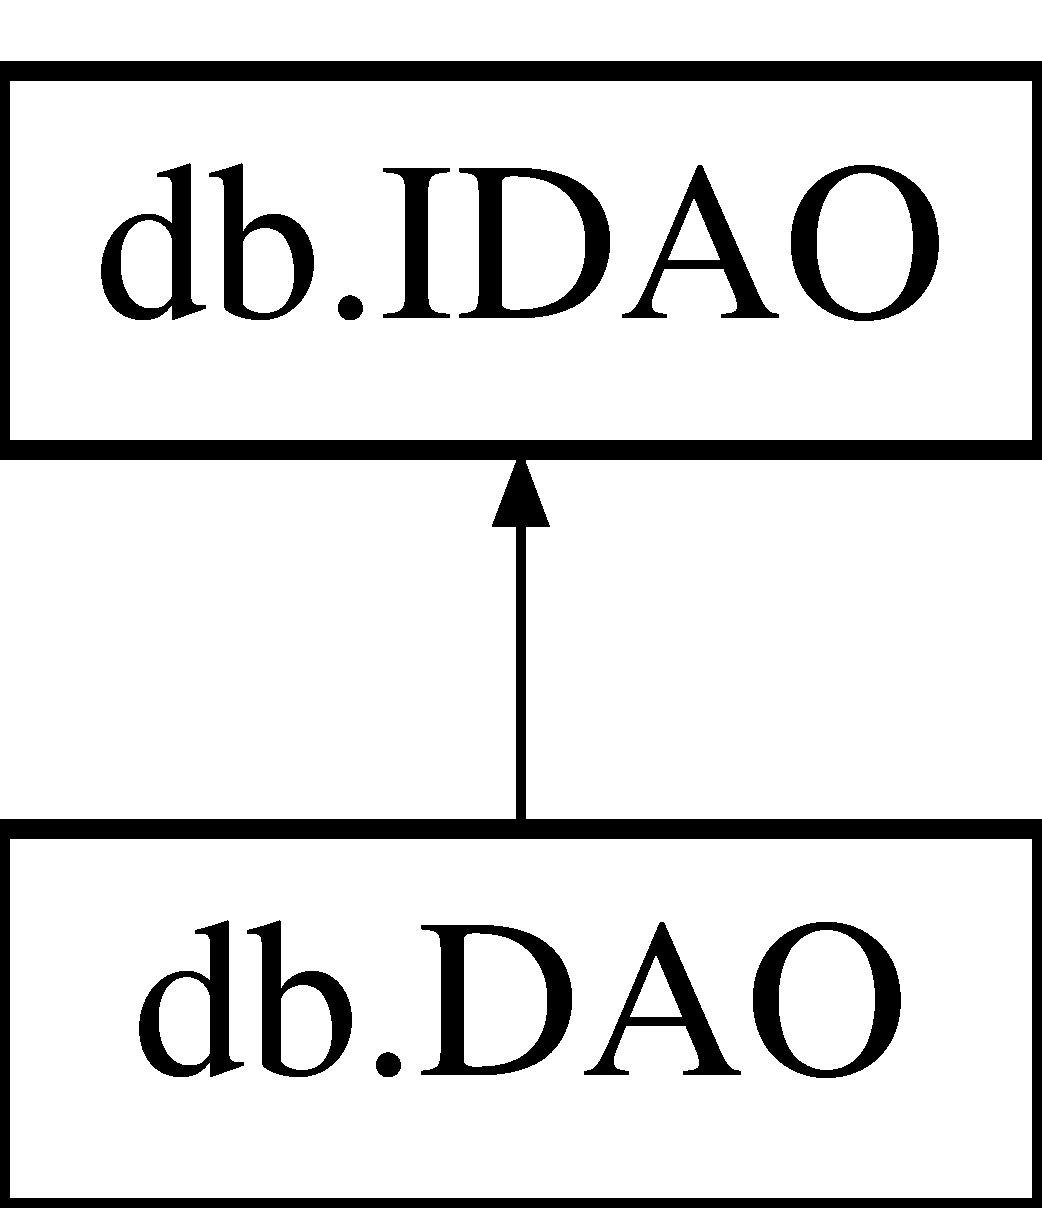
\includegraphics[height=2.000000cm]{interfacedb_1_1_i_d_a_o}
\end{center}
\end{figure}
\subsection*{Public Member Functions}
\begin{DoxyCompactItemize}
\item 
boolean \hyperlink{interfacedb_1_1_i_d_a_o_a5b1f408c9a25305e977e962faa38b026}{store\+User} (\hyperlink{classserver_1_1data_1_1_user}{User} u)
\item 
\hyperlink{classserver_1_1data_1_1_user}{User} \hyperlink{interfacedb_1_1_i_d_a_o_ad00bb5255d0badadbf5244799c3b708f}{retrieve\+User} (String email)
\item 
boolean \hyperlink{interfacedb_1_1_i_d_a_o_adbc5f00b7bcdffb6692367a3c9564193}{update\+User} (\hyperlink{classserver_1_1data_1_1_user}{User} u)
\item 
\hyperlink{classserver_1_1data_1_1_review}{Review} \hyperlink{interfacedb_1_1_i_d_a_o_a53fd20610d94f7c5f0f713dad7528c26}{retrieve\+Review} (int id\+\_\+review)
\item 
boolean \hyperlink{interfacedb_1_1_i_d_a_o_a7288e76ee3ce667c0d0d7ecaeef0d94e}{update\+Review} (\hyperlink{classserver_1_1data_1_1_review}{Review} r)
\item 
boolean \hyperlink{interfacedb_1_1_i_d_a_o_a39851dc1e1f05af40afeb76a5f8be99a}{store\+Book} (\hyperlink{classserver_1_1data_1_1_book}{Book} b)
\item 
\hyperlink{classserver_1_1data_1_1_book}{Book} \hyperlink{interfacedb_1_1_i_d_a_o_a1457ecf91799eaacd17cd3259826fc36}{retrieve\+Book} (int I\+S\+BN)
\item 
boolean \hyperlink{interfacedb_1_1_i_d_a_o_a202354d7a3e1231687d543e82c15a6f5}{update\+Book} (\hyperlink{classserver_1_1data_1_1_book}{Book} b)
\item 
\hyperlink{classserver_1_1data_1_1_book}{Book} \hyperlink{interfacedb_1_1_i_d_a_o_a4c5eda35bfbba1b0a994efe00f99a544}{retrieve\+Book\+By\+Parameter} (String title)
\item 
List$<$ \hyperlink{classserver_1_1data_1_1_user}{User} $>$ \hyperlink{interfacedb_1_1_i_d_a_o_a88b60729d9517ca9aa31b7db7ae07aee}{get\+All\+Users} ()
\item 
List$<$ \hyperlink{classserver_1_1data_1_1_review}{Review} $>$ \hyperlink{interfacedb_1_1_i_d_a_o_a3d9625d7e5426aad3c2e70fd0174e5f0}{get\+All\+Reviews} ()
\item 
List$<$ \hyperlink{classserver_1_1data_1_1_book}{Book} $>$ \hyperlink{interfacedb_1_1_i_d_a_o_a75a5ebcd7c3421ae7cccc8e2f3b2d9f9}{get\+All\+Books} ()
\item 
void \hyperlink{interfacedb_1_1_i_d_a_o_a78ca80bc2f2b660edeb9eddd8ca9a4b7}{delete\+Review} (\hyperlink{classserver_1_1data_1_1_review}{Review} r)
\item 
void \hyperlink{interfacedb_1_1_i_d_a_o_a1d6c98ea794177d7fd12c4a028ec29c1}{delete\+Book} (\hyperlink{classserver_1_1data_1_1_book}{Book} b)
\end{DoxyCompactItemize}


\subsection{Member Function Documentation}
\mbox{\Hypertarget{interfacedb_1_1_i_d_a_o_a1d6c98ea794177d7fd12c4a028ec29c1}\label{interfacedb_1_1_i_d_a_o_a1d6c98ea794177d7fd12c4a028ec29c1}} 
\index{db\+::\+I\+D\+AO@{db\+::\+I\+D\+AO}!delete\+Book@{delete\+Book}}
\index{delete\+Book@{delete\+Book}!db\+::\+I\+D\+AO@{db\+::\+I\+D\+AO}}
\subsubsection{\texorpdfstring{delete\+Book()}{deleteBook()}}
{\footnotesize\ttfamily void db.\+I\+D\+A\+O.\+delete\+Book (\begin{DoxyParamCaption}\item[{\hyperlink{classserver_1_1data_1_1_book}{Book}}]{b }\end{DoxyParamCaption})}



Implemented in \hyperlink{classdb_1_1_d_a_o_a65f6a816c5f6dfb07178daf490f56fdc}{db.\+D\+AO}.

\mbox{\Hypertarget{interfacedb_1_1_i_d_a_o_a78ca80bc2f2b660edeb9eddd8ca9a4b7}\label{interfacedb_1_1_i_d_a_o_a78ca80bc2f2b660edeb9eddd8ca9a4b7}} 
\index{db\+::\+I\+D\+AO@{db\+::\+I\+D\+AO}!delete\+Review@{delete\+Review}}
\index{delete\+Review@{delete\+Review}!db\+::\+I\+D\+AO@{db\+::\+I\+D\+AO}}
\subsubsection{\texorpdfstring{delete\+Review()}{deleteReview()}}
{\footnotesize\ttfamily void db.\+I\+D\+A\+O.\+delete\+Review (\begin{DoxyParamCaption}\item[{\hyperlink{classserver_1_1data_1_1_review}{Review}}]{r }\end{DoxyParamCaption})}



Implemented in \hyperlink{classdb_1_1_d_a_o_aa033f83155deb72d59492bcb2b8e4d3a}{db.\+D\+AO}.

\mbox{\Hypertarget{interfacedb_1_1_i_d_a_o_a75a5ebcd7c3421ae7cccc8e2f3b2d9f9}\label{interfacedb_1_1_i_d_a_o_a75a5ebcd7c3421ae7cccc8e2f3b2d9f9}} 
\index{db\+::\+I\+D\+AO@{db\+::\+I\+D\+AO}!get\+All\+Books@{get\+All\+Books}}
\index{get\+All\+Books@{get\+All\+Books}!db\+::\+I\+D\+AO@{db\+::\+I\+D\+AO}}
\subsubsection{\texorpdfstring{get\+All\+Books()}{getAllBooks()}}
{\footnotesize\ttfamily List$<$\hyperlink{classserver_1_1data_1_1_book}{Book}$>$ db.\+I\+D\+A\+O.\+get\+All\+Books (\begin{DoxyParamCaption}{ }\end{DoxyParamCaption})}



Implemented in \hyperlink{classdb_1_1_d_a_o_a82a8c60ccd0de2f70b69bc36d29aeef8}{db.\+D\+AO}.

\mbox{\Hypertarget{interfacedb_1_1_i_d_a_o_a3d9625d7e5426aad3c2e70fd0174e5f0}\label{interfacedb_1_1_i_d_a_o_a3d9625d7e5426aad3c2e70fd0174e5f0}} 
\index{db\+::\+I\+D\+AO@{db\+::\+I\+D\+AO}!get\+All\+Reviews@{get\+All\+Reviews}}
\index{get\+All\+Reviews@{get\+All\+Reviews}!db\+::\+I\+D\+AO@{db\+::\+I\+D\+AO}}
\subsubsection{\texorpdfstring{get\+All\+Reviews()}{getAllReviews()}}
{\footnotesize\ttfamily List$<$\hyperlink{classserver_1_1data_1_1_review}{Review}$>$ db.\+I\+D\+A\+O.\+get\+All\+Reviews (\begin{DoxyParamCaption}{ }\end{DoxyParamCaption})}



Implemented in \hyperlink{classdb_1_1_d_a_o_a4df79c7d44b050aa55451db2ecf342f6}{db.\+D\+AO}.

\mbox{\Hypertarget{interfacedb_1_1_i_d_a_o_a88b60729d9517ca9aa31b7db7ae07aee}\label{interfacedb_1_1_i_d_a_o_a88b60729d9517ca9aa31b7db7ae07aee}} 
\index{db\+::\+I\+D\+AO@{db\+::\+I\+D\+AO}!get\+All\+Users@{get\+All\+Users}}
\index{get\+All\+Users@{get\+All\+Users}!db\+::\+I\+D\+AO@{db\+::\+I\+D\+AO}}
\subsubsection{\texorpdfstring{get\+All\+Users()}{getAllUsers()}}
{\footnotesize\ttfamily List$<$\hyperlink{classserver_1_1data_1_1_user}{User}$>$ db.\+I\+D\+A\+O.\+get\+All\+Users (\begin{DoxyParamCaption}{ }\end{DoxyParamCaption})}



Implemented in \hyperlink{classdb_1_1_d_a_o_a3b627b7177990799fd02e0c38b8adb70}{db.\+D\+AO}.

\mbox{\Hypertarget{interfacedb_1_1_i_d_a_o_a1457ecf91799eaacd17cd3259826fc36}\label{interfacedb_1_1_i_d_a_o_a1457ecf91799eaacd17cd3259826fc36}} 
\index{db\+::\+I\+D\+AO@{db\+::\+I\+D\+AO}!retrieve\+Book@{retrieve\+Book}}
\index{retrieve\+Book@{retrieve\+Book}!db\+::\+I\+D\+AO@{db\+::\+I\+D\+AO}}
\subsubsection{\texorpdfstring{retrieve\+Book()}{retrieveBook()}}
{\footnotesize\ttfamily \hyperlink{classserver_1_1data_1_1_book}{Book} db.\+I\+D\+A\+O.\+retrieve\+Book (\begin{DoxyParamCaption}\item[{int}]{I\+S\+BN }\end{DoxyParamCaption})}



Implemented in \hyperlink{classdb_1_1_d_a_o_ade778f907d0a74dc27c4fc03f8709815}{db.\+D\+AO}.

\mbox{\Hypertarget{interfacedb_1_1_i_d_a_o_a4c5eda35bfbba1b0a994efe00f99a544}\label{interfacedb_1_1_i_d_a_o_a4c5eda35bfbba1b0a994efe00f99a544}} 
\index{db\+::\+I\+D\+AO@{db\+::\+I\+D\+AO}!retrieve\+Book\+By\+Parameter@{retrieve\+Book\+By\+Parameter}}
\index{retrieve\+Book\+By\+Parameter@{retrieve\+Book\+By\+Parameter}!db\+::\+I\+D\+AO@{db\+::\+I\+D\+AO}}
\subsubsection{\texorpdfstring{retrieve\+Book\+By\+Parameter()}{retrieveBookByParameter()}}
{\footnotesize\ttfamily \hyperlink{classserver_1_1data_1_1_book}{Book} db.\+I\+D\+A\+O.\+retrieve\+Book\+By\+Parameter (\begin{DoxyParamCaption}\item[{String}]{title }\end{DoxyParamCaption})}



Implemented in \hyperlink{classdb_1_1_d_a_o_a1f8580da682f8a8af4896c491c3b6611}{db.\+D\+AO}.

\mbox{\Hypertarget{interfacedb_1_1_i_d_a_o_a53fd20610d94f7c5f0f713dad7528c26}\label{interfacedb_1_1_i_d_a_o_a53fd20610d94f7c5f0f713dad7528c26}} 
\index{db\+::\+I\+D\+AO@{db\+::\+I\+D\+AO}!retrieve\+Review@{retrieve\+Review}}
\index{retrieve\+Review@{retrieve\+Review}!db\+::\+I\+D\+AO@{db\+::\+I\+D\+AO}}
\subsubsection{\texorpdfstring{retrieve\+Review()}{retrieveReview()}}
{\footnotesize\ttfamily \hyperlink{classserver_1_1data_1_1_review}{Review} db.\+I\+D\+A\+O.\+retrieve\+Review (\begin{DoxyParamCaption}\item[{int}]{id\+\_\+review }\end{DoxyParamCaption})}



Implemented in \hyperlink{classdb_1_1_d_a_o_ae43e182fae8ee7028db6ff17c2d5768f}{db.\+D\+AO}.

\mbox{\Hypertarget{interfacedb_1_1_i_d_a_o_ad00bb5255d0badadbf5244799c3b708f}\label{interfacedb_1_1_i_d_a_o_ad00bb5255d0badadbf5244799c3b708f}} 
\index{db\+::\+I\+D\+AO@{db\+::\+I\+D\+AO}!retrieve\+User@{retrieve\+User}}
\index{retrieve\+User@{retrieve\+User}!db\+::\+I\+D\+AO@{db\+::\+I\+D\+AO}}
\subsubsection{\texorpdfstring{retrieve\+User()}{retrieveUser()}}
{\footnotesize\ttfamily \hyperlink{classserver_1_1data_1_1_user}{User} db.\+I\+D\+A\+O.\+retrieve\+User (\begin{DoxyParamCaption}\item[{String}]{email }\end{DoxyParamCaption})}



Implemented in \hyperlink{classdb_1_1_d_a_o_a6da084ffd9b0da23acba9dc68e747303}{db.\+D\+AO}.

\mbox{\Hypertarget{interfacedb_1_1_i_d_a_o_a39851dc1e1f05af40afeb76a5f8be99a}\label{interfacedb_1_1_i_d_a_o_a39851dc1e1f05af40afeb76a5f8be99a}} 
\index{db\+::\+I\+D\+AO@{db\+::\+I\+D\+AO}!store\+Book@{store\+Book}}
\index{store\+Book@{store\+Book}!db\+::\+I\+D\+AO@{db\+::\+I\+D\+AO}}
\subsubsection{\texorpdfstring{store\+Book()}{storeBook()}}
{\footnotesize\ttfamily boolean db.\+I\+D\+A\+O.\+store\+Book (\begin{DoxyParamCaption}\item[{\hyperlink{classserver_1_1data_1_1_book}{Book}}]{b }\end{DoxyParamCaption})}



Implemented in \hyperlink{classdb_1_1_d_a_o_a036246b8124d7ac8a36e3eaafd3eb81a}{db.\+D\+AO}.

\mbox{\Hypertarget{interfacedb_1_1_i_d_a_o_a5b1f408c9a25305e977e962faa38b026}\label{interfacedb_1_1_i_d_a_o_a5b1f408c9a25305e977e962faa38b026}} 
\index{db\+::\+I\+D\+AO@{db\+::\+I\+D\+AO}!store\+User@{store\+User}}
\index{store\+User@{store\+User}!db\+::\+I\+D\+AO@{db\+::\+I\+D\+AO}}
\subsubsection{\texorpdfstring{store\+User()}{storeUser()}}
{\footnotesize\ttfamily boolean db.\+I\+D\+A\+O.\+store\+User (\begin{DoxyParamCaption}\item[{\hyperlink{classserver_1_1data_1_1_user}{User}}]{u }\end{DoxyParamCaption})}



Implemented in \hyperlink{classdb_1_1_d_a_o_a1600c5d7d28eb225fc7c244fdfb16150}{db.\+D\+AO}.

\mbox{\Hypertarget{interfacedb_1_1_i_d_a_o_a202354d7a3e1231687d543e82c15a6f5}\label{interfacedb_1_1_i_d_a_o_a202354d7a3e1231687d543e82c15a6f5}} 
\index{db\+::\+I\+D\+AO@{db\+::\+I\+D\+AO}!update\+Book@{update\+Book}}
\index{update\+Book@{update\+Book}!db\+::\+I\+D\+AO@{db\+::\+I\+D\+AO}}
\subsubsection{\texorpdfstring{update\+Book()}{updateBook()}}
{\footnotesize\ttfamily boolean db.\+I\+D\+A\+O.\+update\+Book (\begin{DoxyParamCaption}\item[{\hyperlink{classserver_1_1data_1_1_book}{Book}}]{b }\end{DoxyParamCaption})}



Implemented in \hyperlink{classdb_1_1_d_a_o_a4ea10c177ef93a3084ed74b38556adca}{db.\+D\+AO}.

\mbox{\Hypertarget{interfacedb_1_1_i_d_a_o_a7288e76ee3ce667c0d0d7ecaeef0d94e}\label{interfacedb_1_1_i_d_a_o_a7288e76ee3ce667c0d0d7ecaeef0d94e}} 
\index{db\+::\+I\+D\+AO@{db\+::\+I\+D\+AO}!update\+Review@{update\+Review}}
\index{update\+Review@{update\+Review}!db\+::\+I\+D\+AO@{db\+::\+I\+D\+AO}}
\subsubsection{\texorpdfstring{update\+Review()}{updateReview()}}
{\footnotesize\ttfamily boolean db.\+I\+D\+A\+O.\+update\+Review (\begin{DoxyParamCaption}\item[{\hyperlink{classserver_1_1data_1_1_review}{Review}}]{r }\end{DoxyParamCaption})}



Implemented in \hyperlink{classdb_1_1_d_a_o_ab73940ac7600902ea7d52bcd041a9c6e}{db.\+D\+AO}.

\mbox{\Hypertarget{interfacedb_1_1_i_d_a_o_adbc5f00b7bcdffb6692367a3c9564193}\label{interfacedb_1_1_i_d_a_o_adbc5f00b7bcdffb6692367a3c9564193}} 
\index{db\+::\+I\+D\+AO@{db\+::\+I\+D\+AO}!update\+User@{update\+User}}
\index{update\+User@{update\+User}!db\+::\+I\+D\+AO@{db\+::\+I\+D\+AO}}
\subsubsection{\texorpdfstring{update\+User()}{updateUser()}}
{\footnotesize\ttfamily boolean db.\+I\+D\+A\+O.\+update\+User (\begin{DoxyParamCaption}\item[{\hyperlink{classserver_1_1data_1_1_user}{User}}]{u }\end{DoxyParamCaption})}



Implemented in \hyperlink{classdb_1_1_d_a_o_a5cd4462deb77065c2d12471cd73b3ec8}{db.\+D\+AO}.



The documentation for this interface was generated from the following file\+:\begin{DoxyCompactItemize}
\item 
src/main/java/db/\hyperlink{_i_d_a_o_8java}{I\+D\+A\+O.\+java}\end{DoxyCompactItemize}

\hypertarget{interfacedb_1_1_i_d_b}{}\section{db.\+I\+DB Interface Reference}
\label{interfacedb_1_1_i_d_b}\index{db.\+I\+DB@{db.\+I\+DB}}
Inheritance diagram for db.\+I\+DB\+:\begin{figure}[H]
\begin{center}
\leavevmode
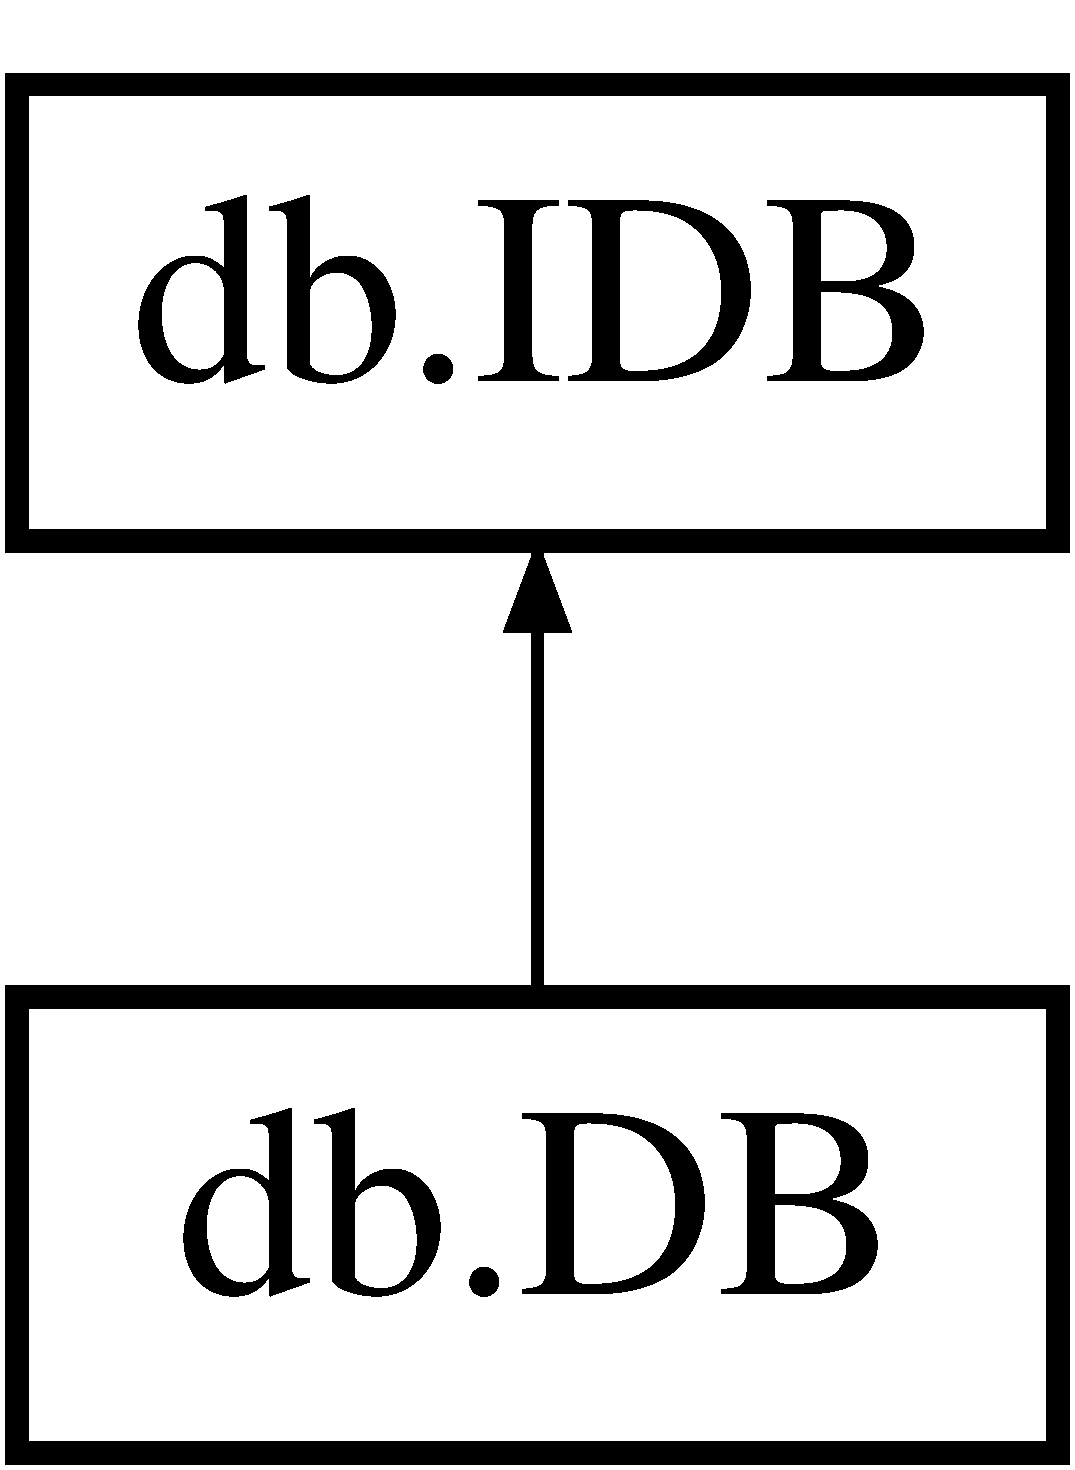
\includegraphics[height=2.000000cm]{interfacedb_1_1_i_d_b}
\end{center}
\end{figure}
\subsection*{Public Member Functions}
\begin{DoxyCompactItemize}
\item 
List$<$ \hyperlink{classserver_1_1data_1_1_user}{User} $>$ \hyperlink{interfacedb_1_1_i_d_b_a39ad15619eae3d0ec652e1849e3ebd50}{get\+All\+Users} ()
\item 
List$<$ \hyperlink{classserver_1_1data_1_1_review}{Review} $>$ \hyperlink{interfacedb_1_1_i_d_b_a08f60c8b923599c650f04b4192d00d55}{get\+All\+Reviews} ()
\item 
List$<$ \hyperlink{classserver_1_1data_1_1_book}{Book} $>$ \hyperlink{interfacedb_1_1_i_d_b_abd0d41674bbcdd524a3ca2403504bf25}{get\+All\+Books} ()
\item 
boolean \hyperlink{interfacedb_1_1_i_d_b_a2ac985a90e8369fab676950b3fb4c2bc}{buy\+Book} (String email, String book\+\_\+title)
\item 
boolean \hyperlink{interfacedb_1_1_i_d_b_a92913d9357ef22978adc35d3fb9d3590}{register\+User} (String email, String password, boolean role)
\item 
boolean \hyperlink{interfacedb_1_1_i_d_b_a63904b26597f651ea6acbd03384e0afb}{add\+Book\+To\+Db} (\hyperlink{classserver_1_1data_1_1_book}{Book} b)
\item 
boolean \hyperlink{interfacedb_1_1_i_d_b_a00a453c6d4fc604615f5a173d86600fc}{add\+Review} (\hyperlink{classserver_1_1data_1_1_book}{Book} b, \hyperlink{classserver_1_1data_1_1_review}{Review} r, \hyperlink{classserver_1_1data_1_1_user}{User} user)
\item 
\hyperlink{classserver_1_1data_1_1_book}{Book} \hyperlink{interfacedb_1_1_i_d_b_aed305f6c36ff140084636a8eded479db}{show\+Book\+By\+I\+S\+BN} (int I\+S\+BN)
\item 
\hyperlink{classserver_1_1data_1_1_book}{Book} \hyperlink{interfacedb_1_1_i_d_b_a6418edaf7c25f99f0422c0000db521fa}{show\+Book\+By\+Title} (String title)
\item 
\hyperlink{classserver_1_1data_1_1_review}{Review} \hyperlink{interfacedb_1_1_i_d_b_a6c44c3135f07ec6dbef84ecc6fe4f90f}{show\+Review} (int id\+\_\+review)
\item 
\hyperlink{classserver_1_1data_1_1_user}{User} \hyperlink{interfacedb_1_1_i_d_b_a8dca82226b1c27ceb4b765259546513d}{show\+User} (String email)
\item 
List$<$ \hyperlink{classserver_1_1data_1_1_review}{Review} $>$ \hyperlink{interfacedb_1_1_i_d_b_afd7ee8924344c13a64a1363d1a295771}{get\+User\+Reviews} (String email)
\item 
List$<$ \hyperlink{classserver_1_1data_1_1_review}{Review} $>$ \hyperlink{interfacedb_1_1_i_d_b_a6b8fda48df77b542b8713bc4f035bccf}{get\+Book\+Reviews} (String title)
\item 
double \hyperlink{interfacedb_1_1_i_d_b_a4d23da2e383e7fe0638089fb2686b6c3}{average\+Rating\+By\+Book} (String title)
\item 
double \hyperlink{interfacedb_1_1_i_d_b_a5bb2209c976ab0a7f20606ed5df0e0cf}{average\+Rating\+By\+User} (String email)
\end{DoxyCompactItemize}


\subsection{Member Function Documentation}
\mbox{\Hypertarget{interfacedb_1_1_i_d_b_a63904b26597f651ea6acbd03384e0afb}\label{interfacedb_1_1_i_d_b_a63904b26597f651ea6acbd03384e0afb}} 
\index{db\+::\+I\+DB@{db\+::\+I\+DB}!add\+Book\+To\+Db@{add\+Book\+To\+Db}}
\index{add\+Book\+To\+Db@{add\+Book\+To\+Db}!db\+::\+I\+DB@{db\+::\+I\+DB}}
\subsubsection{\texorpdfstring{add\+Book\+To\+Db()}{addBookToDb()}}
{\footnotesize\ttfamily boolean db.\+I\+D\+B.\+add\+Book\+To\+Db (\begin{DoxyParamCaption}\item[{\hyperlink{classserver_1_1data_1_1_book}{Book}}]{b }\end{DoxyParamCaption})}



Implemented in \hyperlink{classdb_1_1_d_b_a705ed9c0ffae567ec3ac09fbd7138c6f}{db.\+DB}.

\mbox{\Hypertarget{interfacedb_1_1_i_d_b_a00a453c6d4fc604615f5a173d86600fc}\label{interfacedb_1_1_i_d_b_a00a453c6d4fc604615f5a173d86600fc}} 
\index{db\+::\+I\+DB@{db\+::\+I\+DB}!add\+Review@{add\+Review}}
\index{add\+Review@{add\+Review}!db\+::\+I\+DB@{db\+::\+I\+DB}}
\subsubsection{\texorpdfstring{add\+Review()}{addReview()}}
{\footnotesize\ttfamily boolean db.\+I\+D\+B.\+add\+Review (\begin{DoxyParamCaption}\item[{\hyperlink{classserver_1_1data_1_1_book}{Book}}]{b,  }\item[{\hyperlink{classserver_1_1data_1_1_review}{Review}}]{r,  }\item[{\hyperlink{classserver_1_1data_1_1_user}{User}}]{user }\end{DoxyParamCaption})}



Implemented in \hyperlink{classdb_1_1_d_b_accfa7c2f48252f167576221dc14ff721}{db.\+DB}.

\mbox{\Hypertarget{interfacedb_1_1_i_d_b_a4d23da2e383e7fe0638089fb2686b6c3}\label{interfacedb_1_1_i_d_b_a4d23da2e383e7fe0638089fb2686b6c3}} 
\index{db\+::\+I\+DB@{db\+::\+I\+DB}!average\+Rating\+By\+Book@{average\+Rating\+By\+Book}}
\index{average\+Rating\+By\+Book@{average\+Rating\+By\+Book}!db\+::\+I\+DB@{db\+::\+I\+DB}}
\subsubsection{\texorpdfstring{average\+Rating\+By\+Book()}{averageRatingByBook()}}
{\footnotesize\ttfamily double db.\+I\+D\+B.\+average\+Rating\+By\+Book (\begin{DoxyParamCaption}\item[{String}]{title }\end{DoxyParamCaption})}



Implemented in \hyperlink{classdb_1_1_d_b_a8b2b9d6c4aabb17719e2d2af4cf7ba74}{db.\+DB}.

\mbox{\Hypertarget{interfacedb_1_1_i_d_b_a5bb2209c976ab0a7f20606ed5df0e0cf}\label{interfacedb_1_1_i_d_b_a5bb2209c976ab0a7f20606ed5df0e0cf}} 
\index{db\+::\+I\+DB@{db\+::\+I\+DB}!average\+Rating\+By\+User@{average\+Rating\+By\+User}}
\index{average\+Rating\+By\+User@{average\+Rating\+By\+User}!db\+::\+I\+DB@{db\+::\+I\+DB}}
\subsubsection{\texorpdfstring{average\+Rating\+By\+User()}{averageRatingByUser()}}
{\footnotesize\ttfamily double db.\+I\+D\+B.\+average\+Rating\+By\+User (\begin{DoxyParamCaption}\item[{String}]{email }\end{DoxyParamCaption})}



Implemented in \hyperlink{classdb_1_1_d_b_a38091677ae1e964a84320d6e539ea62e}{db.\+DB}.

\mbox{\Hypertarget{interfacedb_1_1_i_d_b_a2ac985a90e8369fab676950b3fb4c2bc}\label{interfacedb_1_1_i_d_b_a2ac985a90e8369fab676950b3fb4c2bc}} 
\index{db\+::\+I\+DB@{db\+::\+I\+DB}!buy\+Book@{buy\+Book}}
\index{buy\+Book@{buy\+Book}!db\+::\+I\+DB@{db\+::\+I\+DB}}
\subsubsection{\texorpdfstring{buy\+Book()}{buyBook()}}
{\footnotesize\ttfamily boolean db.\+I\+D\+B.\+buy\+Book (\begin{DoxyParamCaption}\item[{String}]{email,  }\item[{String}]{book\+\_\+title }\end{DoxyParamCaption})}



Implemented in \hyperlink{classdb_1_1_d_b_a8a1a15bae4352c3c73092d801ef26c41}{db.\+DB}.

\mbox{\Hypertarget{interfacedb_1_1_i_d_b_abd0d41674bbcdd524a3ca2403504bf25}\label{interfacedb_1_1_i_d_b_abd0d41674bbcdd524a3ca2403504bf25}} 
\index{db\+::\+I\+DB@{db\+::\+I\+DB}!get\+All\+Books@{get\+All\+Books}}
\index{get\+All\+Books@{get\+All\+Books}!db\+::\+I\+DB@{db\+::\+I\+DB}}
\subsubsection{\texorpdfstring{get\+All\+Books()}{getAllBooks()}}
{\footnotesize\ttfamily List$<$\hyperlink{classserver_1_1data_1_1_book}{Book}$>$ db.\+I\+D\+B.\+get\+All\+Books (\begin{DoxyParamCaption}{ }\end{DoxyParamCaption})}



Implemented in \hyperlink{classdb_1_1_d_b_ab4fbfd3716967ce37cc462ca04c68ca8}{db.\+DB}.

\mbox{\Hypertarget{interfacedb_1_1_i_d_b_a08f60c8b923599c650f04b4192d00d55}\label{interfacedb_1_1_i_d_b_a08f60c8b923599c650f04b4192d00d55}} 
\index{db\+::\+I\+DB@{db\+::\+I\+DB}!get\+All\+Reviews@{get\+All\+Reviews}}
\index{get\+All\+Reviews@{get\+All\+Reviews}!db\+::\+I\+DB@{db\+::\+I\+DB}}
\subsubsection{\texorpdfstring{get\+All\+Reviews()}{getAllReviews()}}
{\footnotesize\ttfamily List$<$\hyperlink{classserver_1_1data_1_1_review}{Review}$>$ db.\+I\+D\+B.\+get\+All\+Reviews (\begin{DoxyParamCaption}{ }\end{DoxyParamCaption})}



Implemented in \hyperlink{classdb_1_1_d_b_ac7a84c5621f4ad2263cd830dbf10842e}{db.\+DB}.

\mbox{\Hypertarget{interfacedb_1_1_i_d_b_a39ad15619eae3d0ec652e1849e3ebd50}\label{interfacedb_1_1_i_d_b_a39ad15619eae3d0ec652e1849e3ebd50}} 
\index{db\+::\+I\+DB@{db\+::\+I\+DB}!get\+All\+Users@{get\+All\+Users}}
\index{get\+All\+Users@{get\+All\+Users}!db\+::\+I\+DB@{db\+::\+I\+DB}}
\subsubsection{\texorpdfstring{get\+All\+Users()}{getAllUsers()}}
{\footnotesize\ttfamily List$<$\hyperlink{classserver_1_1data_1_1_user}{User}$>$ db.\+I\+D\+B.\+get\+All\+Users (\begin{DoxyParamCaption}{ }\end{DoxyParamCaption})}



Implemented in \hyperlink{classdb_1_1_d_b_ad02e4c78f9afe64af34fb2e5889ce501}{db.\+DB}.

\mbox{\Hypertarget{interfacedb_1_1_i_d_b_a6b8fda48df77b542b8713bc4f035bccf}\label{interfacedb_1_1_i_d_b_a6b8fda48df77b542b8713bc4f035bccf}} 
\index{db\+::\+I\+DB@{db\+::\+I\+DB}!get\+Book\+Reviews@{get\+Book\+Reviews}}
\index{get\+Book\+Reviews@{get\+Book\+Reviews}!db\+::\+I\+DB@{db\+::\+I\+DB}}
\subsubsection{\texorpdfstring{get\+Book\+Reviews()}{getBookReviews()}}
{\footnotesize\ttfamily List$<$\hyperlink{classserver_1_1data_1_1_review}{Review}$>$ db.\+I\+D\+B.\+get\+Book\+Reviews (\begin{DoxyParamCaption}\item[{String}]{title }\end{DoxyParamCaption})}



Implemented in \hyperlink{classdb_1_1_d_b_a02a42ee97d8e7189733dfc720a05452e}{db.\+DB}.

\mbox{\Hypertarget{interfacedb_1_1_i_d_b_afd7ee8924344c13a64a1363d1a295771}\label{interfacedb_1_1_i_d_b_afd7ee8924344c13a64a1363d1a295771}} 
\index{db\+::\+I\+DB@{db\+::\+I\+DB}!get\+User\+Reviews@{get\+User\+Reviews}}
\index{get\+User\+Reviews@{get\+User\+Reviews}!db\+::\+I\+DB@{db\+::\+I\+DB}}
\subsubsection{\texorpdfstring{get\+User\+Reviews()}{getUserReviews()}}
{\footnotesize\ttfamily List$<$\hyperlink{classserver_1_1data_1_1_review}{Review}$>$ db.\+I\+D\+B.\+get\+User\+Reviews (\begin{DoxyParamCaption}\item[{String}]{email }\end{DoxyParamCaption})}



Implemented in \hyperlink{classdb_1_1_d_b_a9ef4c302b91da17852f09a27a90fb4b5}{db.\+DB}.

\mbox{\Hypertarget{interfacedb_1_1_i_d_b_a92913d9357ef22978adc35d3fb9d3590}\label{interfacedb_1_1_i_d_b_a92913d9357ef22978adc35d3fb9d3590}} 
\index{db\+::\+I\+DB@{db\+::\+I\+DB}!register\+User@{register\+User}}
\index{register\+User@{register\+User}!db\+::\+I\+DB@{db\+::\+I\+DB}}
\subsubsection{\texorpdfstring{register\+User()}{registerUser()}}
{\footnotesize\ttfamily boolean db.\+I\+D\+B.\+register\+User (\begin{DoxyParamCaption}\item[{String}]{email,  }\item[{String}]{password,  }\item[{boolean}]{role }\end{DoxyParamCaption})}



Implemented in \hyperlink{classdb_1_1_d_b_a76fac3ed38eaecd5a073224d6ad51332}{db.\+DB}.

\mbox{\Hypertarget{interfacedb_1_1_i_d_b_aed305f6c36ff140084636a8eded479db}\label{interfacedb_1_1_i_d_b_aed305f6c36ff140084636a8eded479db}} 
\index{db\+::\+I\+DB@{db\+::\+I\+DB}!show\+Book\+By\+I\+S\+BN@{show\+Book\+By\+I\+S\+BN}}
\index{show\+Book\+By\+I\+S\+BN@{show\+Book\+By\+I\+S\+BN}!db\+::\+I\+DB@{db\+::\+I\+DB}}
\subsubsection{\texorpdfstring{show\+Book\+By\+I\+S\+B\+N()}{showBookByISBN()}}
{\footnotesize\ttfamily \hyperlink{classserver_1_1data_1_1_book}{Book} db.\+I\+D\+B.\+show\+Book\+By\+I\+S\+BN (\begin{DoxyParamCaption}\item[{int}]{I\+S\+BN }\end{DoxyParamCaption})}



Implemented in \hyperlink{classdb_1_1_d_b_ae902ce95ca7433f1f7f77419f4121f4c}{db.\+DB}.

\mbox{\Hypertarget{interfacedb_1_1_i_d_b_a6418edaf7c25f99f0422c0000db521fa}\label{interfacedb_1_1_i_d_b_a6418edaf7c25f99f0422c0000db521fa}} 
\index{db\+::\+I\+DB@{db\+::\+I\+DB}!show\+Book\+By\+Title@{show\+Book\+By\+Title}}
\index{show\+Book\+By\+Title@{show\+Book\+By\+Title}!db\+::\+I\+DB@{db\+::\+I\+DB}}
\subsubsection{\texorpdfstring{show\+Book\+By\+Title()}{showBookByTitle()}}
{\footnotesize\ttfamily \hyperlink{classserver_1_1data_1_1_book}{Book} db.\+I\+D\+B.\+show\+Book\+By\+Title (\begin{DoxyParamCaption}\item[{String}]{title }\end{DoxyParamCaption})}



Implemented in \hyperlink{classdb_1_1_d_b_a22a4c5b98facd4506b03828697220773}{db.\+DB}.

\mbox{\Hypertarget{interfacedb_1_1_i_d_b_a6c44c3135f07ec6dbef84ecc6fe4f90f}\label{interfacedb_1_1_i_d_b_a6c44c3135f07ec6dbef84ecc6fe4f90f}} 
\index{db\+::\+I\+DB@{db\+::\+I\+DB}!show\+Review@{show\+Review}}
\index{show\+Review@{show\+Review}!db\+::\+I\+DB@{db\+::\+I\+DB}}
\subsubsection{\texorpdfstring{show\+Review()}{showReview()}}
{\footnotesize\ttfamily \hyperlink{classserver_1_1data_1_1_review}{Review} db.\+I\+D\+B.\+show\+Review (\begin{DoxyParamCaption}\item[{int}]{id\+\_\+review }\end{DoxyParamCaption})}



Implemented in \hyperlink{classdb_1_1_d_b_a84b36a9e2c155b1aa2868844cd157df7}{db.\+DB}.

\mbox{\Hypertarget{interfacedb_1_1_i_d_b_a8dca82226b1c27ceb4b765259546513d}\label{interfacedb_1_1_i_d_b_a8dca82226b1c27ceb4b765259546513d}} 
\index{db\+::\+I\+DB@{db\+::\+I\+DB}!show\+User@{show\+User}}
\index{show\+User@{show\+User}!db\+::\+I\+DB@{db\+::\+I\+DB}}
\subsubsection{\texorpdfstring{show\+User()}{showUser()}}
{\footnotesize\ttfamily \hyperlink{classserver_1_1data_1_1_user}{User} db.\+I\+D\+B.\+show\+User (\begin{DoxyParamCaption}\item[{String}]{email }\end{DoxyParamCaption})}



Implemented in \hyperlink{classdb_1_1_d_b_a914986669ac622ef33ae344baaefa32c}{db.\+DB}.



The documentation for this interface was generated from the following file\+:\begin{DoxyCompactItemize}
\item 
src/main/java/db/\hyperlink{_i_d_b_8java}{I\+D\+B.\+java}\end{DoxyCompactItemize}

\hypertarget{interfaceserver_1_1remote_1_1_i_remote}{}\section{server.\+remote.\+I\+Remote Interface Reference}
\label{interfaceserver_1_1remote_1_1_i_remote}\index{server.\+remote.\+I\+Remote@{server.\+remote.\+I\+Remote}}
Inheritance diagram for server.\+remote.\+I\+Remote\+:\begin{figure}[H]
\begin{center}
\leavevmode
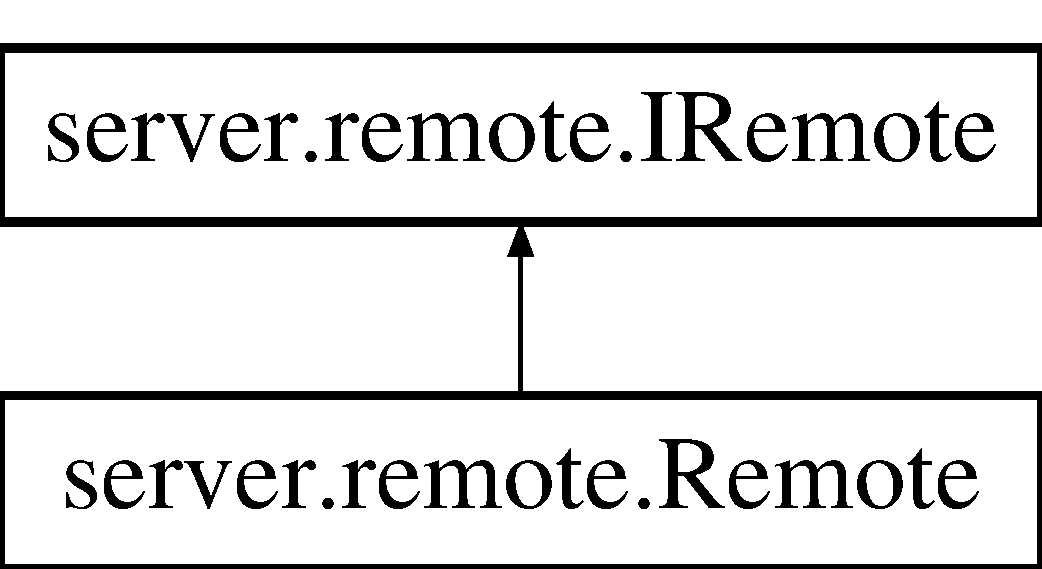
\includegraphics[height=2.000000cm]{interfaceserver_1_1remote_1_1_i_remote}
\end{center}
\end{figure}
\subsection*{Public Member Functions}
\begin{DoxyCompactItemize}
\item 
boolean \hyperlink{interfaceserver_1_1remote_1_1_i_remote_a2e426f5eb58352993207ce0a24539f81}{register\+User} (String email, String password, boolean role)  throws Remote\+Exception
\item 
boolean \hyperlink{interfaceserver_1_1remote_1_1_i_remote_a3b11a0e182873e445ec8546394e36373}{add\+Book} (\hyperlink{classserver_1_1data_1_1_book}{Book} book)  throws Remote\+Exception
\item 
List$<$ \hyperlink{classserver_1_1data_1_1_book}{Book} $>$ \hyperlink{interfaceserver_1_1remote_1_1_i_remote_ac8a764235c51eff20d635f40707e377e}{show\+Books\+In\+Store} ()  throws Remote\+Exception
\item 
List$<$ \hyperlink{classserver_1_1data_1_1_user}{User} $>$ \hyperlink{interfaceserver_1_1remote_1_1_i_remote_a3ff8752a1911b6ca54fc4a04af90fe7a}{get\+All\+Users} ()  throws Remote\+Exception
\item 
List$<$ \hyperlink{classserver_1_1data_1_1_review}{Review} $>$ \hyperlink{interfaceserver_1_1remote_1_1_i_remote_a017e07cb93ae582188c20d7b1ce6b014}{get\+All\+Reviews} ()  throws Remote\+Exception
\item 
\hyperlink{classserver_1_1data_1_1_book}{Book} \hyperlink{interfaceserver_1_1remote_1_1_i_remote_a7d561f9f92fb53177f2d3e49e445148a}{book\+Test} ()  throws Remote\+Exception
\item 
\hyperlink{classserver_1_1data_1_1_book}{Book} \hyperlink{interfaceserver_1_1remote_1_1_i_remote_a736183bf7a57f78acf11fb78ae0f0e58}{get\+Book\+By\+I\+S\+BN} (int I\+S\+BN)  throws Remote\+Exception
\item 
\hyperlink{classserver_1_1data_1_1_book}{Book} \hyperlink{interfaceserver_1_1remote_1_1_i_remote_a520cc1af90d13264c14b32e19b5ce712}{get\+Book\+By\+Title} (String title)  throws Remote\+Exception
\item 
\hyperlink{classserver_1_1data_1_1_review}{Review} \hyperlink{interfaceserver_1_1remote_1_1_i_remote_a7b3462a438579c85dc7f097acf9cec41}{get\+Review} (int id\+\_\+review)  throws Remote\+Exception
\item 
\hyperlink{classserver_1_1data_1_1_user}{User} \hyperlink{interfaceserver_1_1remote_1_1_i_remote_ab741cf58a7e2b18ba36069d14d9d04ef}{get\+User} (String email)  throws Remote\+Exception
\item 
boolean \hyperlink{interfaceserver_1_1remote_1_1_i_remote_a5ecb918e7d2650346770f3ff5676c25b}{buy\+Book} (String email, String book\+\_\+title)  throws Remote\+Exception
\item 
boolean \hyperlink{interfaceserver_1_1remote_1_1_i_remote_ab24486281e8c228ee82a48a5ca70297b}{add\+Review} (\hyperlink{classserver_1_1data_1_1_book}{Book} b, \hyperlink{classserver_1_1data_1_1_review}{Review} r, \hyperlink{classserver_1_1data_1_1_user}{User} u)  throws Remote\+Exception
\item 
List$<$ \hyperlink{classserver_1_1data_1_1_review}{Review} $>$ \hyperlink{interfaceserver_1_1remote_1_1_i_remote_a9e52d282ba2386018ebd6817459a743f}{get\+User\+Reviews} (String email)  throws Remote\+Exception
\item 
List$<$ \hyperlink{classserver_1_1data_1_1_review}{Review} $>$ \hyperlink{interfaceserver_1_1remote_1_1_i_remote_a600254593b70d9757190475d3435b390}{get\+Book\+Reviews} (String title)  throws Remote\+Exception
\item 
double \hyperlink{interfaceserver_1_1remote_1_1_i_remote_a4a53942c94debc835f1817b2753722de}{average\+Rating\+By\+Book} (String title)  throws Remote\+Exception
\item 
double \hyperlink{interfaceserver_1_1remote_1_1_i_remote_a11c915f0c22728be1898d46a78ac92cf}{average\+Rating\+By\+User} (String email)  throws Remote\+Exception
\end{DoxyCompactItemize}


\subsection{Member Function Documentation}
\mbox{\Hypertarget{interfaceserver_1_1remote_1_1_i_remote_a3b11a0e182873e445ec8546394e36373}\label{interfaceserver_1_1remote_1_1_i_remote_a3b11a0e182873e445ec8546394e36373}} 
\index{server\+::remote\+::\+I\+Remote@{server\+::remote\+::\+I\+Remote}!add\+Book@{add\+Book}}
\index{add\+Book@{add\+Book}!server\+::remote\+::\+I\+Remote@{server\+::remote\+::\+I\+Remote}}
\subsubsection{\texorpdfstring{add\+Book()}{addBook()}}
{\footnotesize\ttfamily boolean server.\+remote.\+I\+Remote.\+add\+Book (\begin{DoxyParamCaption}\item[{\hyperlink{classserver_1_1data_1_1_book}{Book}}]{book }\end{DoxyParamCaption}) throws Remote\+Exception}



Implemented in \hyperlink{classserver_1_1remote_1_1_remote_a496fcecd259c1b527ffba62fc452afee}{server.\+remote.\+Remote}.

\mbox{\Hypertarget{interfaceserver_1_1remote_1_1_i_remote_ab24486281e8c228ee82a48a5ca70297b}\label{interfaceserver_1_1remote_1_1_i_remote_ab24486281e8c228ee82a48a5ca70297b}} 
\index{server\+::remote\+::\+I\+Remote@{server\+::remote\+::\+I\+Remote}!add\+Review@{add\+Review}}
\index{add\+Review@{add\+Review}!server\+::remote\+::\+I\+Remote@{server\+::remote\+::\+I\+Remote}}
\subsubsection{\texorpdfstring{add\+Review()}{addReview()}}
{\footnotesize\ttfamily boolean server.\+remote.\+I\+Remote.\+add\+Review (\begin{DoxyParamCaption}\item[{\hyperlink{classserver_1_1data_1_1_book}{Book}}]{b,  }\item[{\hyperlink{classserver_1_1data_1_1_review}{Review}}]{r,  }\item[{\hyperlink{classserver_1_1data_1_1_user}{User}}]{u }\end{DoxyParamCaption}) throws Remote\+Exception}



Implemented in \hyperlink{classserver_1_1remote_1_1_remote_af94163cf6d5c40cfc880eb517d56aa48}{server.\+remote.\+Remote}.

\mbox{\Hypertarget{interfaceserver_1_1remote_1_1_i_remote_a4a53942c94debc835f1817b2753722de}\label{interfaceserver_1_1remote_1_1_i_remote_a4a53942c94debc835f1817b2753722de}} 
\index{server\+::remote\+::\+I\+Remote@{server\+::remote\+::\+I\+Remote}!average\+Rating\+By\+Book@{average\+Rating\+By\+Book}}
\index{average\+Rating\+By\+Book@{average\+Rating\+By\+Book}!server\+::remote\+::\+I\+Remote@{server\+::remote\+::\+I\+Remote}}
\subsubsection{\texorpdfstring{average\+Rating\+By\+Book()}{averageRatingByBook()}}
{\footnotesize\ttfamily double server.\+remote.\+I\+Remote.\+average\+Rating\+By\+Book (\begin{DoxyParamCaption}\item[{String}]{title }\end{DoxyParamCaption}) throws Remote\+Exception}



Implemented in \hyperlink{classserver_1_1remote_1_1_remote_afd253ddc199a34a1e05317878f957cc9}{server.\+remote.\+Remote}.

\mbox{\Hypertarget{interfaceserver_1_1remote_1_1_i_remote_a11c915f0c22728be1898d46a78ac92cf}\label{interfaceserver_1_1remote_1_1_i_remote_a11c915f0c22728be1898d46a78ac92cf}} 
\index{server\+::remote\+::\+I\+Remote@{server\+::remote\+::\+I\+Remote}!average\+Rating\+By\+User@{average\+Rating\+By\+User}}
\index{average\+Rating\+By\+User@{average\+Rating\+By\+User}!server\+::remote\+::\+I\+Remote@{server\+::remote\+::\+I\+Remote}}
\subsubsection{\texorpdfstring{average\+Rating\+By\+User()}{averageRatingByUser()}}
{\footnotesize\ttfamily double server.\+remote.\+I\+Remote.\+average\+Rating\+By\+User (\begin{DoxyParamCaption}\item[{String}]{email }\end{DoxyParamCaption}) throws Remote\+Exception}



Implemented in \hyperlink{classserver_1_1remote_1_1_remote_a67fc7aeeb889a80cda6e1a5f83858c2a}{server.\+remote.\+Remote}.

\mbox{\Hypertarget{interfaceserver_1_1remote_1_1_i_remote_a7d561f9f92fb53177f2d3e49e445148a}\label{interfaceserver_1_1remote_1_1_i_remote_a7d561f9f92fb53177f2d3e49e445148a}} 
\index{server\+::remote\+::\+I\+Remote@{server\+::remote\+::\+I\+Remote}!book\+Test@{book\+Test}}
\index{book\+Test@{book\+Test}!server\+::remote\+::\+I\+Remote@{server\+::remote\+::\+I\+Remote}}
\subsubsection{\texorpdfstring{book\+Test()}{bookTest()}}
{\footnotesize\ttfamily \hyperlink{classserver_1_1data_1_1_book}{Book} server.\+remote.\+I\+Remote.\+book\+Test (\begin{DoxyParamCaption}{ }\end{DoxyParamCaption}) throws Remote\+Exception}



Implemented in \hyperlink{classserver_1_1remote_1_1_remote_a38bce20fa59064fe8d970164d6155435}{server.\+remote.\+Remote}.

\mbox{\Hypertarget{interfaceserver_1_1remote_1_1_i_remote_a5ecb918e7d2650346770f3ff5676c25b}\label{interfaceserver_1_1remote_1_1_i_remote_a5ecb918e7d2650346770f3ff5676c25b}} 
\index{server\+::remote\+::\+I\+Remote@{server\+::remote\+::\+I\+Remote}!buy\+Book@{buy\+Book}}
\index{buy\+Book@{buy\+Book}!server\+::remote\+::\+I\+Remote@{server\+::remote\+::\+I\+Remote}}
\subsubsection{\texorpdfstring{buy\+Book()}{buyBook()}}
{\footnotesize\ttfamily boolean server.\+remote.\+I\+Remote.\+buy\+Book (\begin{DoxyParamCaption}\item[{String}]{email,  }\item[{String}]{book\+\_\+title }\end{DoxyParamCaption}) throws Remote\+Exception}



Implemented in \hyperlink{classserver_1_1remote_1_1_remote_af5d1abb1730b8db14ab9dd476df158d8}{server.\+remote.\+Remote}.

\mbox{\Hypertarget{interfaceserver_1_1remote_1_1_i_remote_a017e07cb93ae582188c20d7b1ce6b014}\label{interfaceserver_1_1remote_1_1_i_remote_a017e07cb93ae582188c20d7b1ce6b014}} 
\index{server\+::remote\+::\+I\+Remote@{server\+::remote\+::\+I\+Remote}!get\+All\+Reviews@{get\+All\+Reviews}}
\index{get\+All\+Reviews@{get\+All\+Reviews}!server\+::remote\+::\+I\+Remote@{server\+::remote\+::\+I\+Remote}}
\subsubsection{\texorpdfstring{get\+All\+Reviews()}{getAllReviews()}}
{\footnotesize\ttfamily List$<$\hyperlink{classserver_1_1data_1_1_review}{Review}$>$ server.\+remote.\+I\+Remote.\+get\+All\+Reviews (\begin{DoxyParamCaption}{ }\end{DoxyParamCaption}) throws Remote\+Exception}



Implemented in \hyperlink{classserver_1_1remote_1_1_remote_a22538e64b45f5f93237b455100243b44}{server.\+remote.\+Remote}.

\mbox{\Hypertarget{interfaceserver_1_1remote_1_1_i_remote_a3ff8752a1911b6ca54fc4a04af90fe7a}\label{interfaceserver_1_1remote_1_1_i_remote_a3ff8752a1911b6ca54fc4a04af90fe7a}} 
\index{server\+::remote\+::\+I\+Remote@{server\+::remote\+::\+I\+Remote}!get\+All\+Users@{get\+All\+Users}}
\index{get\+All\+Users@{get\+All\+Users}!server\+::remote\+::\+I\+Remote@{server\+::remote\+::\+I\+Remote}}
\subsubsection{\texorpdfstring{get\+All\+Users()}{getAllUsers()}}
{\footnotesize\ttfamily List$<$\hyperlink{classserver_1_1data_1_1_user}{User}$>$ server.\+remote.\+I\+Remote.\+get\+All\+Users (\begin{DoxyParamCaption}{ }\end{DoxyParamCaption}) throws Remote\+Exception}



Implemented in \hyperlink{classserver_1_1remote_1_1_remote_a3d41acc8ab7328be2082573542758f07}{server.\+remote.\+Remote}.

\mbox{\Hypertarget{interfaceserver_1_1remote_1_1_i_remote_a736183bf7a57f78acf11fb78ae0f0e58}\label{interfaceserver_1_1remote_1_1_i_remote_a736183bf7a57f78acf11fb78ae0f0e58}} 
\index{server\+::remote\+::\+I\+Remote@{server\+::remote\+::\+I\+Remote}!get\+Book\+By\+I\+S\+BN@{get\+Book\+By\+I\+S\+BN}}
\index{get\+Book\+By\+I\+S\+BN@{get\+Book\+By\+I\+S\+BN}!server\+::remote\+::\+I\+Remote@{server\+::remote\+::\+I\+Remote}}
\subsubsection{\texorpdfstring{get\+Book\+By\+I\+S\+B\+N()}{getBookByISBN()}}
{\footnotesize\ttfamily \hyperlink{classserver_1_1data_1_1_book}{Book} server.\+remote.\+I\+Remote.\+get\+Book\+By\+I\+S\+BN (\begin{DoxyParamCaption}\item[{int}]{I\+S\+BN }\end{DoxyParamCaption}) throws Remote\+Exception}



Implemented in \hyperlink{classserver_1_1remote_1_1_remote_a36ffc6f95ea75ad7d393ea296e1bc0cc}{server.\+remote.\+Remote}.

\mbox{\Hypertarget{interfaceserver_1_1remote_1_1_i_remote_a520cc1af90d13264c14b32e19b5ce712}\label{interfaceserver_1_1remote_1_1_i_remote_a520cc1af90d13264c14b32e19b5ce712}} 
\index{server\+::remote\+::\+I\+Remote@{server\+::remote\+::\+I\+Remote}!get\+Book\+By\+Title@{get\+Book\+By\+Title}}
\index{get\+Book\+By\+Title@{get\+Book\+By\+Title}!server\+::remote\+::\+I\+Remote@{server\+::remote\+::\+I\+Remote}}
\subsubsection{\texorpdfstring{get\+Book\+By\+Title()}{getBookByTitle()}}
{\footnotesize\ttfamily \hyperlink{classserver_1_1data_1_1_book}{Book} server.\+remote.\+I\+Remote.\+get\+Book\+By\+Title (\begin{DoxyParamCaption}\item[{String}]{title }\end{DoxyParamCaption}) throws Remote\+Exception}



Implemented in \hyperlink{classserver_1_1remote_1_1_remote_a560427fc017e15f04e12bd880e6f086e}{server.\+remote.\+Remote}.

\mbox{\Hypertarget{interfaceserver_1_1remote_1_1_i_remote_a600254593b70d9757190475d3435b390}\label{interfaceserver_1_1remote_1_1_i_remote_a600254593b70d9757190475d3435b390}} 
\index{server\+::remote\+::\+I\+Remote@{server\+::remote\+::\+I\+Remote}!get\+Book\+Reviews@{get\+Book\+Reviews}}
\index{get\+Book\+Reviews@{get\+Book\+Reviews}!server\+::remote\+::\+I\+Remote@{server\+::remote\+::\+I\+Remote}}
\subsubsection{\texorpdfstring{get\+Book\+Reviews()}{getBookReviews()}}
{\footnotesize\ttfamily List$<$\hyperlink{classserver_1_1data_1_1_review}{Review}$>$ server.\+remote.\+I\+Remote.\+get\+Book\+Reviews (\begin{DoxyParamCaption}\item[{String}]{title }\end{DoxyParamCaption}) throws Remote\+Exception}



Implemented in \hyperlink{classserver_1_1remote_1_1_remote_a501e5c5fe847917c9615f0772864a147}{server.\+remote.\+Remote}.

\mbox{\Hypertarget{interfaceserver_1_1remote_1_1_i_remote_a7b3462a438579c85dc7f097acf9cec41}\label{interfaceserver_1_1remote_1_1_i_remote_a7b3462a438579c85dc7f097acf9cec41}} 
\index{server\+::remote\+::\+I\+Remote@{server\+::remote\+::\+I\+Remote}!get\+Review@{get\+Review}}
\index{get\+Review@{get\+Review}!server\+::remote\+::\+I\+Remote@{server\+::remote\+::\+I\+Remote}}
\subsubsection{\texorpdfstring{get\+Review()}{getReview()}}
{\footnotesize\ttfamily \hyperlink{classserver_1_1data_1_1_review}{Review} server.\+remote.\+I\+Remote.\+get\+Review (\begin{DoxyParamCaption}\item[{int}]{id\+\_\+review }\end{DoxyParamCaption}) throws Remote\+Exception}



Implemented in \hyperlink{classserver_1_1remote_1_1_remote_a98bd7181568c637a6cbcc0b72ebb9f95}{server.\+remote.\+Remote}.

\mbox{\Hypertarget{interfaceserver_1_1remote_1_1_i_remote_ab741cf58a7e2b18ba36069d14d9d04ef}\label{interfaceserver_1_1remote_1_1_i_remote_ab741cf58a7e2b18ba36069d14d9d04ef}} 
\index{server\+::remote\+::\+I\+Remote@{server\+::remote\+::\+I\+Remote}!get\+User@{get\+User}}
\index{get\+User@{get\+User}!server\+::remote\+::\+I\+Remote@{server\+::remote\+::\+I\+Remote}}
\subsubsection{\texorpdfstring{get\+User()}{getUser()}}
{\footnotesize\ttfamily \hyperlink{classserver_1_1data_1_1_user}{User} server.\+remote.\+I\+Remote.\+get\+User (\begin{DoxyParamCaption}\item[{String}]{email }\end{DoxyParamCaption}) throws Remote\+Exception}



Implemented in \hyperlink{classserver_1_1remote_1_1_remote_abef8350014445d8f2d5ffb4c088e82b6}{server.\+remote.\+Remote}.

\mbox{\Hypertarget{interfaceserver_1_1remote_1_1_i_remote_a9e52d282ba2386018ebd6817459a743f}\label{interfaceserver_1_1remote_1_1_i_remote_a9e52d282ba2386018ebd6817459a743f}} 
\index{server\+::remote\+::\+I\+Remote@{server\+::remote\+::\+I\+Remote}!get\+User\+Reviews@{get\+User\+Reviews}}
\index{get\+User\+Reviews@{get\+User\+Reviews}!server\+::remote\+::\+I\+Remote@{server\+::remote\+::\+I\+Remote}}
\subsubsection{\texorpdfstring{get\+User\+Reviews()}{getUserReviews()}}
{\footnotesize\ttfamily List$<$\hyperlink{classserver_1_1data_1_1_review}{Review}$>$ server.\+remote.\+I\+Remote.\+get\+User\+Reviews (\begin{DoxyParamCaption}\item[{String}]{email }\end{DoxyParamCaption}) throws Remote\+Exception}



Implemented in \hyperlink{classserver_1_1remote_1_1_remote_a396c96a6b8802c2b4658ecccd37e84db}{server.\+remote.\+Remote}.

\mbox{\Hypertarget{interfaceserver_1_1remote_1_1_i_remote_a2e426f5eb58352993207ce0a24539f81}\label{interfaceserver_1_1remote_1_1_i_remote_a2e426f5eb58352993207ce0a24539f81}} 
\index{server\+::remote\+::\+I\+Remote@{server\+::remote\+::\+I\+Remote}!register\+User@{register\+User}}
\index{register\+User@{register\+User}!server\+::remote\+::\+I\+Remote@{server\+::remote\+::\+I\+Remote}}
\subsubsection{\texorpdfstring{register\+User()}{registerUser()}}
{\footnotesize\ttfamily boolean server.\+remote.\+I\+Remote.\+register\+User (\begin{DoxyParamCaption}\item[{String}]{email,  }\item[{String}]{password,  }\item[{boolean}]{role }\end{DoxyParamCaption}) throws Remote\+Exception}



Implemented in \hyperlink{classserver_1_1remote_1_1_remote_ad3a381123e93a8e5ec26d84c4ff8b92f}{server.\+remote.\+Remote}.

\mbox{\Hypertarget{interfaceserver_1_1remote_1_1_i_remote_ac8a764235c51eff20d635f40707e377e}\label{interfaceserver_1_1remote_1_1_i_remote_ac8a764235c51eff20d635f40707e377e}} 
\index{server\+::remote\+::\+I\+Remote@{server\+::remote\+::\+I\+Remote}!show\+Books\+In\+Store@{show\+Books\+In\+Store}}
\index{show\+Books\+In\+Store@{show\+Books\+In\+Store}!server\+::remote\+::\+I\+Remote@{server\+::remote\+::\+I\+Remote}}
\subsubsection{\texorpdfstring{show\+Books\+In\+Store()}{showBooksInStore()}}
{\footnotesize\ttfamily List$<$\hyperlink{classserver_1_1data_1_1_book}{Book}$>$ server.\+remote.\+I\+Remote.\+show\+Books\+In\+Store (\begin{DoxyParamCaption}{ }\end{DoxyParamCaption}) throws Remote\+Exception}



Implemented in \hyperlink{classserver_1_1remote_1_1_remote_a131873c01bc4fe829dd7d2385c89ca87}{server.\+remote.\+Remote}.



The documentation for this interface was generated from the following file\+:\begin{DoxyCompactItemize}
\item 
src/main/java/server/remote/\hyperlink{_i_remote_8java}{I\+Remote.\+java}\end{DoxyCompactItemize}

\hypertarget{classclient_1_1gui_1_1_log_in}{}\section{client.\+gui.\+Log\+In Class Reference}
\label{classclient_1_1gui_1_1_log_in}\index{client.\+gui.\+Log\+In@{client.\+gui.\+Log\+In}}
\subsection*{Public Member Functions}
\begin{DoxyCompactItemize}
\item 
\hyperlink{classclient_1_1gui_1_1_log_in_a035e2ad40bb6d0fdc8041cc895a6b959}{Log\+In} ()
\end{DoxyCompactItemize}
\subsection*{Static Public Member Functions}
\begin{DoxyCompactItemize}
\item 
static void \hyperlink{classclient_1_1gui_1_1_log_in_a5bff6d5c81be59bf4aecb55182417f8a}{main} (String\mbox{[}$\,$\mbox{]} args)
\end{DoxyCompactItemize}


\subsection{Constructor \& Destructor Documentation}
\mbox{\Hypertarget{classclient_1_1gui_1_1_log_in_a035e2ad40bb6d0fdc8041cc895a6b959}\label{classclient_1_1gui_1_1_log_in_a035e2ad40bb6d0fdc8041cc895a6b959}} 
\index{client\+::gui\+::\+Log\+In@{client\+::gui\+::\+Log\+In}!Log\+In@{Log\+In}}
\index{Log\+In@{Log\+In}!client\+::gui\+::\+Log\+In@{client\+::gui\+::\+Log\+In}}
\subsubsection{\texorpdfstring{Log\+In()}{LogIn()}}
{\footnotesize\ttfamily client.\+gui.\+Log\+In.\+Log\+In (\begin{DoxyParamCaption}{ }\end{DoxyParamCaption})}

Create the application. 

\subsection{Member Function Documentation}
\mbox{\Hypertarget{classclient_1_1gui_1_1_log_in_a5bff6d5c81be59bf4aecb55182417f8a}\label{classclient_1_1gui_1_1_log_in_a5bff6d5c81be59bf4aecb55182417f8a}} 
\index{client\+::gui\+::\+Log\+In@{client\+::gui\+::\+Log\+In}!main@{main}}
\index{main@{main}!client\+::gui\+::\+Log\+In@{client\+::gui\+::\+Log\+In}}
\subsubsection{\texorpdfstring{main()}{main()}}
{\footnotesize\ttfamily static void client.\+gui.\+Log\+In.\+main (\begin{DoxyParamCaption}\item[{String \mbox{[}$\,$\mbox{]}}]{args }\end{DoxyParamCaption})\hspace{0.3cm}{\ttfamily [static]}}



The documentation for this class was generated from the following file\+:\begin{DoxyCompactItemize}
\item 
src/main/java/client/gui/\hyperlink{_log_in_8java}{Log\+In.\+java}\end{DoxyCompactItemize}

\hypertarget{classserver_1_1remote_1_1_remote}{}\section{server.\+remote.\+Remote Class Reference}
\label{classserver_1_1remote_1_1_remote}\index{server.\+remote.\+Remote@{server.\+remote.\+Remote}}
Inheritance diagram for server.\+remote.\+Remote\+:\begin{figure}[H]
\begin{center}
\leavevmode
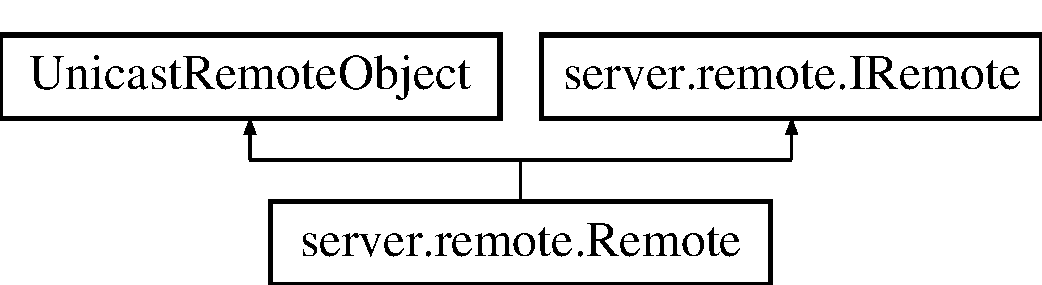
\includegraphics[height=2.000000cm]{classserver_1_1remote_1_1_remote}
\end{center}
\end{figure}
\subsection*{Public Member Functions}
\begin{DoxyCompactItemize}
\item 
\hyperlink{classserver_1_1remote_1_1_remote_a023cdc695c53195005bf645a97307529}{Remote} ()  throws Remote\+Exception 
\item 
boolean \hyperlink{classserver_1_1remote_1_1_remote_ad3a381123e93a8e5ec26d84c4ff8b92f}{register\+User} (String email, String password, boolean role)  throws Remote\+Exception 
\item 
List$<$ \hyperlink{classserver_1_1data_1_1_book}{Book} $>$ \hyperlink{classserver_1_1remote_1_1_remote_a131873c01bc4fe829dd7d2385c89ca87}{show\+Books\+In\+Store} ()  throws Remote\+Exception 
\item 
List$<$ \hyperlink{classserver_1_1data_1_1_user}{User} $>$ \hyperlink{classserver_1_1remote_1_1_remote_a3d41acc8ab7328be2082573542758f07}{get\+All\+Users} ()  throws Remote\+Exception 
\item 
boolean \hyperlink{classserver_1_1remote_1_1_remote_a496fcecd259c1b527ffba62fc452afee}{add\+Book} (\hyperlink{classserver_1_1data_1_1_book}{Book} book)  throws Remote\+Exception
\item 
List$<$ \hyperlink{classserver_1_1data_1_1_review}{Review} $>$ \hyperlink{classserver_1_1remote_1_1_remote_a22538e64b45f5f93237b455100243b44}{get\+All\+Reviews} ()  throws Remote\+Exception 
\item 
\hyperlink{classserver_1_1data_1_1_book}{Book} \hyperlink{classserver_1_1remote_1_1_remote_a38bce20fa59064fe8d970164d6155435}{book\+Test} ()
\item 
\hyperlink{classserver_1_1data_1_1_book}{Book} \hyperlink{classserver_1_1remote_1_1_remote_a36ffc6f95ea75ad7d393ea296e1bc0cc}{get\+Book\+By\+I\+S\+BN} (int I\+S\+BN)  throws Remote\+Exception
\item 
\hyperlink{classserver_1_1data_1_1_book}{Book} \hyperlink{classserver_1_1remote_1_1_remote_a560427fc017e15f04e12bd880e6f086e}{get\+Book\+By\+Title} (String title)  throws Remote\+Exception
\item 
\hyperlink{classserver_1_1data_1_1_review}{Review} \hyperlink{classserver_1_1remote_1_1_remote_a98bd7181568c637a6cbcc0b72ebb9f95}{get\+Review} (int id\+\_\+review)  throws Remote\+Exception 
\item 
\hyperlink{classserver_1_1data_1_1_user}{User} \hyperlink{classserver_1_1remote_1_1_remote_abef8350014445d8f2d5ffb4c088e82b6}{get\+User} (String email)  throws Remote\+Exception 
\item 
boolean \hyperlink{classserver_1_1remote_1_1_remote_af5d1abb1730b8db14ab9dd476df158d8}{buy\+Book} (String email, String book\+\_\+title)  throws Remote\+Exception
\item 
boolean \hyperlink{classserver_1_1remote_1_1_remote_af94163cf6d5c40cfc880eb517d56aa48}{add\+Review} (\hyperlink{classserver_1_1data_1_1_book}{Book} b, \hyperlink{classserver_1_1data_1_1_review}{Review} r, \hyperlink{classserver_1_1data_1_1_user}{User} u)
\item 
List$<$ \hyperlink{classserver_1_1data_1_1_review}{Review} $>$ \hyperlink{classserver_1_1remote_1_1_remote_a396c96a6b8802c2b4658ecccd37e84db}{get\+User\+Reviews} (String email)
\item 
List$<$ \hyperlink{classserver_1_1data_1_1_review}{Review} $>$ \hyperlink{classserver_1_1remote_1_1_remote_a501e5c5fe847917c9615f0772864a147}{get\+Book\+Reviews} (String title)
\item 
double \hyperlink{classserver_1_1remote_1_1_remote_afd253ddc199a34a1e05317878f957cc9}{average\+Rating\+By\+Book} (String title)
\item 
double \hyperlink{classserver_1_1remote_1_1_remote_a67fc7aeeb889a80cda6e1a5f83858c2a}{average\+Rating\+By\+User} (String email)
\item 
void \hyperlink{classserver_1_1remote_1_1_remote_ab80b5addc446fe5f1ecf9a522794ff4f}{delete\+Review} (int id\+\_\+review)
\item 
void \hyperlink{classserver_1_1remote_1_1_remote_a013ab36d40de824c6ad7a48f59d12684}{delete\+Book} (int I\+S\+BN)
\item 
boolean \hyperlink{classserver_1_1remote_1_1_remote_afd807d8743560106c61a01094795c9cb}{add\+Book} (int I\+S\+BN, String title, String category, String edition, String author, double price, String description, String img)
\end{DoxyCompactItemize}


\subsection{Constructor \& Destructor Documentation}
\mbox{\Hypertarget{classserver_1_1remote_1_1_remote_a023cdc695c53195005bf645a97307529}\label{classserver_1_1remote_1_1_remote_a023cdc695c53195005bf645a97307529}} 
\index{server\+::remote\+::\+Remote@{server\+::remote\+::\+Remote}!Remote@{Remote}}
\index{Remote@{Remote}!server\+::remote\+::\+Remote@{server\+::remote\+::\+Remote}}
\subsubsection{\texorpdfstring{Remote()}{Remote()}}
{\footnotesize\ttfamily server.\+remote.\+Remote.\+Remote (\begin{DoxyParamCaption}{ }\end{DoxyParamCaption}) throws Remote\+Exception}



\subsection{Member Function Documentation}
\mbox{\Hypertarget{classserver_1_1remote_1_1_remote_a496fcecd259c1b527ffba62fc452afee}\label{classserver_1_1remote_1_1_remote_a496fcecd259c1b527ffba62fc452afee}} 
\index{server\+::remote\+::\+Remote@{server\+::remote\+::\+Remote}!add\+Book@{add\+Book}}
\index{add\+Book@{add\+Book}!server\+::remote\+::\+Remote@{server\+::remote\+::\+Remote}}
\subsubsection{\texorpdfstring{add\+Book()}{addBook()}\hspace{0.1cm}{\footnotesize\ttfamily [1/2]}}
{\footnotesize\ttfamily boolean server.\+remote.\+Remote.\+add\+Book (\begin{DoxyParamCaption}\item[{\hyperlink{classserver_1_1data_1_1_book}{Book}}]{book }\end{DoxyParamCaption}) throws Remote\+Exception}

adds a book to the database 
\begin{DoxyParams}{Parameters}
{\em book} & \\
\hline
\end{DoxyParams}
\begin{DoxyReturn}{Returns}
true or false to tell if it worked 
\end{DoxyReturn}

\begin{DoxyExceptions}{Exceptions}
{\em Remote\+Exception} & \\
\hline
\end{DoxyExceptions}


Implements \hyperlink{interfaceserver_1_1remote_1_1_i_remote_a3b11a0e182873e445ec8546394e36373}{server.\+remote.\+I\+Remote}.

\mbox{\Hypertarget{classserver_1_1remote_1_1_remote_afd807d8743560106c61a01094795c9cb}\label{classserver_1_1remote_1_1_remote_afd807d8743560106c61a01094795c9cb}} 
\index{server\+::remote\+::\+Remote@{server\+::remote\+::\+Remote}!add\+Book@{add\+Book}}
\index{add\+Book@{add\+Book}!server\+::remote\+::\+Remote@{server\+::remote\+::\+Remote}}
\subsubsection{\texorpdfstring{add\+Book()}{addBook()}\hspace{0.1cm}{\footnotesize\ttfamily [2/2]}}
{\footnotesize\ttfamily boolean server.\+remote.\+Remote.\+add\+Book (\begin{DoxyParamCaption}\item[{int}]{I\+S\+BN,  }\item[{String}]{title,  }\item[{String}]{category,  }\item[{String}]{edition,  }\item[{String}]{author,  }\item[{double}]{price,  }\item[{String}]{description,  }\item[{String}]{img }\end{DoxyParamCaption})}

\begin{DoxyReturn}{Returns}
boolean true if the book is created and stored in db 
\end{DoxyReturn}


Implements \hyperlink{interfaceserver_1_1remote_1_1_i_remote_aec137a7435ccced1aa7350b2fd2a1947}{server.\+remote.\+I\+Remote}.

\mbox{\Hypertarget{classserver_1_1remote_1_1_remote_af94163cf6d5c40cfc880eb517d56aa48}\label{classserver_1_1remote_1_1_remote_af94163cf6d5c40cfc880eb517d56aa48}} 
\index{server\+::remote\+::\+Remote@{server\+::remote\+::\+Remote}!add\+Review@{add\+Review}}
\index{add\+Review@{add\+Review}!server\+::remote\+::\+Remote@{server\+::remote\+::\+Remote}}
\subsubsection{\texorpdfstring{add\+Review()}{addReview()}}
{\footnotesize\ttfamily boolean server.\+remote.\+Remote.\+add\+Review (\begin{DoxyParamCaption}\item[{\hyperlink{classserver_1_1data_1_1_book}{Book}}]{b,  }\item[{\hyperlink{classserver_1_1data_1_1_review}{Review}}]{r,  }\item[{\hyperlink{classserver_1_1data_1_1_user}{User}}]{u }\end{DoxyParamCaption})}

add a new review to a book 
\begin{DoxyParams}{Parameters}
{\em b} & the book to add a review \\
\hline
{\em r} & the Review \\
\hline
{\em u} & the User who made the review \\
\hline
\end{DoxyParams}
\begin{DoxyReturn}{Returns}
true of false to tell if it worked 
\end{DoxyReturn}

\begin{DoxyExceptions}{Exceptions}
{\em Remote\+Exception} & \\
\hline
\end{DoxyExceptions}


Implements \hyperlink{interfaceserver_1_1remote_1_1_i_remote_ab24486281e8c228ee82a48a5ca70297b}{server.\+remote.\+I\+Remote}.

\mbox{\Hypertarget{classserver_1_1remote_1_1_remote_afd253ddc199a34a1e05317878f957cc9}\label{classserver_1_1remote_1_1_remote_afd253ddc199a34a1e05317878f957cc9}} 
\index{server\+::remote\+::\+Remote@{server\+::remote\+::\+Remote}!average\+Rating\+By\+Book@{average\+Rating\+By\+Book}}
\index{average\+Rating\+By\+Book@{average\+Rating\+By\+Book}!server\+::remote\+::\+Remote@{server\+::remote\+::\+Remote}}
\subsubsection{\texorpdfstring{average\+Rating\+By\+Book()}{averageRatingByBook()}}
{\footnotesize\ttfamily double server.\+remote.\+Remote.\+average\+Rating\+By\+Book (\begin{DoxyParamCaption}\item[{String}]{title }\end{DoxyParamCaption})}

Get the average Rating of a book 
\begin{DoxyParams}{Parameters}
{\em title} & of the book \\
\hline
\end{DoxyParams}
\begin{DoxyReturn}{Returns}
a double 
\end{DoxyReturn}

\begin{DoxyExceptions}{Exceptions}
{\em Remote\+Exception} & \\
\hline
\end{DoxyExceptions}


Implements \hyperlink{interfaceserver_1_1remote_1_1_i_remote_a4a53942c94debc835f1817b2753722de}{server.\+remote.\+I\+Remote}.

\mbox{\Hypertarget{classserver_1_1remote_1_1_remote_a67fc7aeeb889a80cda6e1a5f83858c2a}\label{classserver_1_1remote_1_1_remote_a67fc7aeeb889a80cda6e1a5f83858c2a}} 
\index{server\+::remote\+::\+Remote@{server\+::remote\+::\+Remote}!average\+Rating\+By\+User@{average\+Rating\+By\+User}}
\index{average\+Rating\+By\+User@{average\+Rating\+By\+User}!server\+::remote\+::\+Remote@{server\+::remote\+::\+Remote}}
\subsubsection{\texorpdfstring{average\+Rating\+By\+User()}{averageRatingByUser()}}
{\footnotesize\ttfamily double server.\+remote.\+Remote.\+average\+Rating\+By\+User (\begin{DoxyParamCaption}\item[{String}]{email }\end{DoxyParamCaption})}

Get the average Rating given by a User 
\begin{DoxyParams}{Parameters}
{\em email} & \\
\hline
\end{DoxyParams}
\begin{DoxyReturn}{Returns}
a double 
\end{DoxyReturn}

\begin{DoxyExceptions}{Exceptions}
{\em Remote\+Exception} & \\
\hline
\end{DoxyExceptions}


Implements \hyperlink{interfaceserver_1_1remote_1_1_i_remote_a11c915f0c22728be1898d46a78ac92cf}{server.\+remote.\+I\+Remote}.

\mbox{\Hypertarget{classserver_1_1remote_1_1_remote_a38bce20fa59064fe8d970164d6155435}\label{classserver_1_1remote_1_1_remote_a38bce20fa59064fe8d970164d6155435}} 
\index{server\+::remote\+::\+Remote@{server\+::remote\+::\+Remote}!book\+Test@{book\+Test}}
\index{book\+Test@{book\+Test}!server\+::remote\+::\+Remote@{server\+::remote\+::\+Remote}}
\subsubsection{\texorpdfstring{book\+Test()}{bookTest()}}
{\footnotesize\ttfamily \hyperlink{classserver_1_1data_1_1_book}{Book} server.\+remote.\+Remote.\+book\+Test (\begin{DoxyParamCaption}{ }\end{DoxyParamCaption})}

Test \begin{DoxyReturn}{Returns}
the test book 
\end{DoxyReturn}

\begin{DoxyExceptions}{Exceptions}
{\em Remote\+Exception} & \\
\hline
\end{DoxyExceptions}


Implements \hyperlink{interfaceserver_1_1remote_1_1_i_remote_a7d561f9f92fb53177f2d3e49e445148a}{server.\+remote.\+I\+Remote}.

\mbox{\Hypertarget{classserver_1_1remote_1_1_remote_af5d1abb1730b8db14ab9dd476df158d8}\label{classserver_1_1remote_1_1_remote_af5d1abb1730b8db14ab9dd476df158d8}} 
\index{server\+::remote\+::\+Remote@{server\+::remote\+::\+Remote}!buy\+Book@{buy\+Book}}
\index{buy\+Book@{buy\+Book}!server\+::remote\+::\+Remote@{server\+::remote\+::\+Remote}}
\subsubsection{\texorpdfstring{buy\+Book()}{buyBook()}}
{\footnotesize\ttfamily boolean server.\+remote.\+Remote.\+buy\+Book (\begin{DoxyParamCaption}\item[{String}]{email,  }\item[{String}]{book\+\_\+title }\end{DoxyParamCaption}) throws Remote\+Exception}

Buy a book 
\begin{DoxyParams}{Parameters}
{\em email} & of the user \\
\hline
{\em book\+\_\+title} & title of the book \\
\hline
\end{DoxyParams}
\begin{DoxyReturn}{Returns}
true of false to tell if it worked 
\end{DoxyReturn}

\begin{DoxyExceptions}{Exceptions}
{\em Remote\+Exception} & \\
\hline
\end{DoxyExceptions}


Implements \hyperlink{interfaceserver_1_1remote_1_1_i_remote_a5ecb918e7d2650346770f3ff5676c25b}{server.\+remote.\+I\+Remote}.

\mbox{\Hypertarget{classserver_1_1remote_1_1_remote_a013ab36d40de824c6ad7a48f59d12684}\label{classserver_1_1remote_1_1_remote_a013ab36d40de824c6ad7a48f59d12684}} 
\index{server\+::remote\+::\+Remote@{server\+::remote\+::\+Remote}!delete\+Book@{delete\+Book}}
\index{delete\+Book@{delete\+Book}!server\+::remote\+::\+Remote@{server\+::remote\+::\+Remote}}
\subsubsection{\texorpdfstring{delete\+Book()}{deleteBook()}}
{\footnotesize\ttfamily void server.\+remote.\+Remote.\+delete\+Book (\begin{DoxyParamCaption}\item[{int}]{I\+S\+BN }\end{DoxyParamCaption})}

Eliminates a Book 
\begin{DoxyParams}{Parameters}
{\em I\+S\+BN} & \\
\hline
\end{DoxyParams}

\begin{DoxyExceptions}{Exceptions}
{\em Remote\+Exception} & \\
\hline
\end{DoxyExceptions}


Implements \hyperlink{interfaceserver_1_1remote_1_1_i_remote_ac64967dff86a9c603d0c9eb815f222df}{server.\+remote.\+I\+Remote}.

\mbox{\Hypertarget{classserver_1_1remote_1_1_remote_ab80b5addc446fe5f1ecf9a522794ff4f}\label{classserver_1_1remote_1_1_remote_ab80b5addc446fe5f1ecf9a522794ff4f}} 
\index{server\+::remote\+::\+Remote@{server\+::remote\+::\+Remote}!delete\+Review@{delete\+Review}}
\index{delete\+Review@{delete\+Review}!server\+::remote\+::\+Remote@{server\+::remote\+::\+Remote}}
\subsubsection{\texorpdfstring{delete\+Review()}{deleteReview()}}
{\footnotesize\ttfamily void server.\+remote.\+Remote.\+delete\+Review (\begin{DoxyParamCaption}\item[{int}]{id\+\_\+review }\end{DoxyParamCaption})}

Eliminates a Review 
\begin{DoxyParams}{Parameters}
{\em id\+\_\+review} & \\
\hline
\end{DoxyParams}

\begin{DoxyExceptions}{Exceptions}
{\em Remote\+Exception} & \\
\hline
\end{DoxyExceptions}


Implements \hyperlink{interfaceserver_1_1remote_1_1_i_remote_a2bcc3db515d7b6f420449bcf6367298c}{server.\+remote.\+I\+Remote}.

\mbox{\Hypertarget{classserver_1_1remote_1_1_remote_a22538e64b45f5f93237b455100243b44}\label{classserver_1_1remote_1_1_remote_a22538e64b45f5f93237b455100243b44}} 
\index{server\+::remote\+::\+Remote@{server\+::remote\+::\+Remote}!get\+All\+Reviews@{get\+All\+Reviews}}
\index{get\+All\+Reviews@{get\+All\+Reviews}!server\+::remote\+::\+Remote@{server\+::remote\+::\+Remote}}
\subsubsection{\texorpdfstring{get\+All\+Reviews()}{getAllReviews()}}
{\footnotesize\ttfamily List$<$\hyperlink{classserver_1_1data_1_1_review}{Review}$>$ server.\+remote.\+Remote.\+get\+All\+Reviews (\begin{DoxyParamCaption}{ }\end{DoxyParamCaption}) throws Remote\+Exception}

gives you a all the Review in the database \begin{DoxyReturn}{Returns}
a list$<$\+Review$>$ with all the books in the database 
\end{DoxyReturn}

\begin{DoxyExceptions}{Exceptions}
{\em Remote\+Exception} & \\
\hline
\end{DoxyExceptions}


Implements \hyperlink{interfaceserver_1_1remote_1_1_i_remote_a017e07cb93ae582188c20d7b1ce6b014}{server.\+remote.\+I\+Remote}.

\mbox{\Hypertarget{classserver_1_1remote_1_1_remote_a3d41acc8ab7328be2082573542758f07}\label{classserver_1_1remote_1_1_remote_a3d41acc8ab7328be2082573542758f07}} 
\index{server\+::remote\+::\+Remote@{server\+::remote\+::\+Remote}!get\+All\+Users@{get\+All\+Users}}
\index{get\+All\+Users@{get\+All\+Users}!server\+::remote\+::\+Remote@{server\+::remote\+::\+Remote}}
\subsubsection{\texorpdfstring{get\+All\+Users()}{getAllUsers()}}
{\footnotesize\ttfamily List$<$\hyperlink{classserver_1_1data_1_1_user}{User}$>$ server.\+remote.\+Remote.\+get\+All\+Users (\begin{DoxyParamCaption}{ }\end{DoxyParamCaption}) throws Remote\+Exception}

gives you a all the users in the database \begin{DoxyReturn}{Returns}
a list$<$\+User$>$ with all the users in the database 
\end{DoxyReturn}

\begin{DoxyExceptions}{Exceptions}
{\em Remote\+Exception} & \\
\hline
\end{DoxyExceptions}


Implements \hyperlink{interfaceserver_1_1remote_1_1_i_remote_a3ff8752a1911b6ca54fc4a04af90fe7a}{server.\+remote.\+I\+Remote}.

\mbox{\Hypertarget{classserver_1_1remote_1_1_remote_a36ffc6f95ea75ad7d393ea296e1bc0cc}\label{classserver_1_1remote_1_1_remote_a36ffc6f95ea75ad7d393ea296e1bc0cc}} 
\index{server\+::remote\+::\+Remote@{server\+::remote\+::\+Remote}!get\+Book\+By\+I\+S\+BN@{get\+Book\+By\+I\+S\+BN}}
\index{get\+Book\+By\+I\+S\+BN@{get\+Book\+By\+I\+S\+BN}!server\+::remote\+::\+Remote@{server\+::remote\+::\+Remote}}
\subsubsection{\texorpdfstring{get\+Book\+By\+I\+S\+B\+N()}{getBookByISBN()}}
{\footnotesize\ttfamily \hyperlink{classserver_1_1data_1_1_book}{Book} server.\+remote.\+Remote.\+get\+Book\+By\+I\+S\+BN (\begin{DoxyParamCaption}\item[{int}]{I\+S\+BN }\end{DoxyParamCaption}) throws Remote\+Exception}

Get a book by its I\+S\+BN 
\begin{DoxyParams}{Parameters}
{\em I\+S\+BN} & unique book ID \\
\hline
\end{DoxyParams}
\begin{DoxyReturn}{Returns}
a Book with the selected I\+S\+BN 
\end{DoxyReturn}

\begin{DoxyExceptions}{Exceptions}
{\em Remote\+Exception} & \\
\hline
\end{DoxyExceptions}


Implements \hyperlink{interfaceserver_1_1remote_1_1_i_remote_a736183bf7a57f78acf11fb78ae0f0e58}{server.\+remote.\+I\+Remote}.

\mbox{\Hypertarget{classserver_1_1remote_1_1_remote_a560427fc017e15f04e12bd880e6f086e}\label{classserver_1_1remote_1_1_remote_a560427fc017e15f04e12bd880e6f086e}} 
\index{server\+::remote\+::\+Remote@{server\+::remote\+::\+Remote}!get\+Book\+By\+Title@{get\+Book\+By\+Title}}
\index{get\+Book\+By\+Title@{get\+Book\+By\+Title}!server\+::remote\+::\+Remote@{server\+::remote\+::\+Remote}}
\subsubsection{\texorpdfstring{get\+Book\+By\+Title()}{getBookByTitle()}}
{\footnotesize\ttfamily \hyperlink{classserver_1_1data_1_1_book}{Book} server.\+remote.\+Remote.\+get\+Book\+By\+Title (\begin{DoxyParamCaption}\item[{String}]{title }\end{DoxyParamCaption}) throws Remote\+Exception}

Get a Book by its title 
\begin{DoxyParams}{Parameters}
{\em title} & name of the book \\
\hline
\end{DoxyParams}
\begin{DoxyReturn}{Returns}
a Book with the selected Title 
\end{DoxyReturn}

\begin{DoxyExceptions}{Exceptions}
{\em Remote\+Exception} & \\
\hline
\end{DoxyExceptions}


Implements \hyperlink{interfaceserver_1_1remote_1_1_i_remote_a520cc1af90d13264c14b32e19b5ce712}{server.\+remote.\+I\+Remote}.

\mbox{\Hypertarget{classserver_1_1remote_1_1_remote_a501e5c5fe847917c9615f0772864a147}\label{classserver_1_1remote_1_1_remote_a501e5c5fe847917c9615f0772864a147}} 
\index{server\+::remote\+::\+Remote@{server\+::remote\+::\+Remote}!get\+Book\+Reviews@{get\+Book\+Reviews}}
\index{get\+Book\+Reviews@{get\+Book\+Reviews}!server\+::remote\+::\+Remote@{server\+::remote\+::\+Remote}}
\subsubsection{\texorpdfstring{get\+Book\+Reviews()}{getBookReviews()}}
{\footnotesize\ttfamily List$<$\hyperlink{classserver_1_1data_1_1_review}{Review}$>$ server.\+remote.\+Remote.\+get\+Book\+Reviews (\begin{DoxyParamCaption}\item[{String}]{title }\end{DoxyParamCaption})}

Get all the Reviews of a Book 
\begin{DoxyParams}{Parameters}
{\em title} & of the book \\
\hline
\end{DoxyParams}
\begin{DoxyReturn}{Returns}
List$<$\+Review$>$ 
\end{DoxyReturn}

\begin{DoxyExceptions}{Exceptions}
{\em Remote\+Exception} & \\
\hline
\end{DoxyExceptions}


Implements \hyperlink{interfaceserver_1_1remote_1_1_i_remote_a600254593b70d9757190475d3435b390}{server.\+remote.\+I\+Remote}.

\mbox{\Hypertarget{classserver_1_1remote_1_1_remote_a98bd7181568c637a6cbcc0b72ebb9f95}\label{classserver_1_1remote_1_1_remote_a98bd7181568c637a6cbcc0b72ebb9f95}} 
\index{server\+::remote\+::\+Remote@{server\+::remote\+::\+Remote}!get\+Review@{get\+Review}}
\index{get\+Review@{get\+Review}!server\+::remote\+::\+Remote@{server\+::remote\+::\+Remote}}
\subsubsection{\texorpdfstring{get\+Review()}{getReview()}}
{\footnotesize\ttfamily \hyperlink{classserver_1_1data_1_1_review}{Review} server.\+remote.\+Remote.\+get\+Review (\begin{DoxyParamCaption}\item[{int}]{id\+\_\+review }\end{DoxyParamCaption}) throws Remote\+Exception}

Get a Review by its ID 
\begin{DoxyParams}{Parameters}
{\em id\+\_\+review} & unique number \\
\hline
\end{DoxyParams}
\begin{DoxyReturn}{Returns}
a Review 
\end{DoxyReturn}

\begin{DoxyExceptions}{Exceptions}
{\em Remote\+Exception} & \\
\hline
\end{DoxyExceptions}


Implements \hyperlink{interfaceserver_1_1remote_1_1_i_remote_a7b3462a438579c85dc7f097acf9cec41}{server.\+remote.\+I\+Remote}.

\mbox{\Hypertarget{classserver_1_1remote_1_1_remote_abef8350014445d8f2d5ffb4c088e82b6}\label{classserver_1_1remote_1_1_remote_abef8350014445d8f2d5ffb4c088e82b6}} 
\index{server\+::remote\+::\+Remote@{server\+::remote\+::\+Remote}!get\+User@{get\+User}}
\index{get\+User@{get\+User}!server\+::remote\+::\+Remote@{server\+::remote\+::\+Remote}}
\subsubsection{\texorpdfstring{get\+User()}{getUser()}}
{\footnotesize\ttfamily \hyperlink{classserver_1_1data_1_1_user}{User} server.\+remote.\+Remote.\+get\+User (\begin{DoxyParamCaption}\item[{String}]{email }\end{DoxyParamCaption}) throws Remote\+Exception}

Get a User by its Email 
\begin{DoxyParams}{Parameters}
{\em email} & \\
\hline
\end{DoxyParams}
\begin{DoxyReturn}{Returns}
a User 
\end{DoxyReturn}

\begin{DoxyExceptions}{Exceptions}
{\em Remote\+Exception} & \\
\hline
\end{DoxyExceptions}


Implements \hyperlink{interfaceserver_1_1remote_1_1_i_remote_ab741cf58a7e2b18ba36069d14d9d04ef}{server.\+remote.\+I\+Remote}.

\mbox{\Hypertarget{classserver_1_1remote_1_1_remote_a396c96a6b8802c2b4658ecccd37e84db}\label{classserver_1_1remote_1_1_remote_a396c96a6b8802c2b4658ecccd37e84db}} 
\index{server\+::remote\+::\+Remote@{server\+::remote\+::\+Remote}!get\+User\+Reviews@{get\+User\+Reviews}}
\index{get\+User\+Reviews@{get\+User\+Reviews}!server\+::remote\+::\+Remote@{server\+::remote\+::\+Remote}}
\subsubsection{\texorpdfstring{get\+User\+Reviews()}{getUserReviews()}}
{\footnotesize\ttfamily List$<$\hyperlink{classserver_1_1data_1_1_review}{Review}$>$ server.\+remote.\+Remote.\+get\+User\+Reviews (\begin{DoxyParamCaption}\item[{String}]{email }\end{DoxyParamCaption})}

Get all the Reviews a User Made 
\begin{DoxyParams}{Parameters}
{\em email} & of the user \\
\hline
\end{DoxyParams}
\begin{DoxyReturn}{Returns}
a List$<$\+Review$>$ 
\end{DoxyReturn}

\begin{DoxyExceptions}{Exceptions}
{\em Remote\+Exception} & \\
\hline
\end{DoxyExceptions}


Implements \hyperlink{interfaceserver_1_1remote_1_1_i_remote_a9e52d282ba2386018ebd6817459a743f}{server.\+remote.\+I\+Remote}.

\mbox{\Hypertarget{classserver_1_1remote_1_1_remote_ad3a381123e93a8e5ec26d84c4ff8b92f}\label{classserver_1_1remote_1_1_remote_ad3a381123e93a8e5ec26d84c4ff8b92f}} 
\index{server\+::remote\+::\+Remote@{server\+::remote\+::\+Remote}!register\+User@{register\+User}}
\index{register\+User@{register\+User}!server\+::remote\+::\+Remote@{server\+::remote\+::\+Remote}}
\subsubsection{\texorpdfstring{register\+User()}{registerUser()}}
{\footnotesize\ttfamily boolean server.\+remote.\+Remote.\+register\+User (\begin{DoxyParamCaption}\item[{String}]{email,  }\item[{String}]{password,  }\item[{boolean}]{role }\end{DoxyParamCaption}) throws Remote\+Exception}

creates a new user 
\begin{DoxyParams}{Parameters}
{\em email} & \\
\hline
{\em password} & \\
\hline
{\em role} & (true admin; false user) \\
\hline
\end{DoxyParams}
\begin{DoxyReturn}{Returns}
true or false to tell if it worked 
\end{DoxyReturn}

\begin{DoxyExceptions}{Exceptions}
{\em Remote\+Exception} & \\
\hline
\end{DoxyExceptions}


Implements \hyperlink{interfaceserver_1_1remote_1_1_i_remote_a2e426f5eb58352993207ce0a24539f81}{server.\+remote.\+I\+Remote}.

\mbox{\Hypertarget{classserver_1_1remote_1_1_remote_a131873c01bc4fe829dd7d2385c89ca87}\label{classserver_1_1remote_1_1_remote_a131873c01bc4fe829dd7d2385c89ca87}} 
\index{server\+::remote\+::\+Remote@{server\+::remote\+::\+Remote}!show\+Books\+In\+Store@{show\+Books\+In\+Store}}
\index{show\+Books\+In\+Store@{show\+Books\+In\+Store}!server\+::remote\+::\+Remote@{server\+::remote\+::\+Remote}}
\subsubsection{\texorpdfstring{show\+Books\+In\+Store()}{showBooksInStore()}}
{\footnotesize\ttfamily List$<$\hyperlink{classserver_1_1data_1_1_book}{Book}$>$ server.\+remote.\+Remote.\+show\+Books\+In\+Store (\begin{DoxyParamCaption}{ }\end{DoxyParamCaption}) throws Remote\+Exception}

gives you a all the books in the database \begin{DoxyReturn}{Returns}
a list$<$\+Book$>$ with all the books in the database 
\end{DoxyReturn}

\begin{DoxyExceptions}{Exceptions}
{\em Remote\+Exception} & \\
\hline
\end{DoxyExceptions}


Implements \hyperlink{interfaceserver_1_1remote_1_1_i_remote_ac8a764235c51eff20d635f40707e377e}{server.\+remote.\+I\+Remote}.



The documentation for this class was generated from the following file\+:\begin{DoxyCompactItemize}
\item 
src/main/java/server/remote/\hyperlink{_remote_8java}{Remote.\+java}\end{DoxyCompactItemize}

\hypertarget{classserver_1_1data_1_1_review}{}\section{server.\+data.\+Review Class Reference}
\label{classserver_1_1data_1_1_review}\index{server.\+data.\+Review@{server.\+data.\+Review}}
Inheritance diagram for server.\+data.\+Review\+:\begin{figure}[H]
\begin{center}
\leavevmode
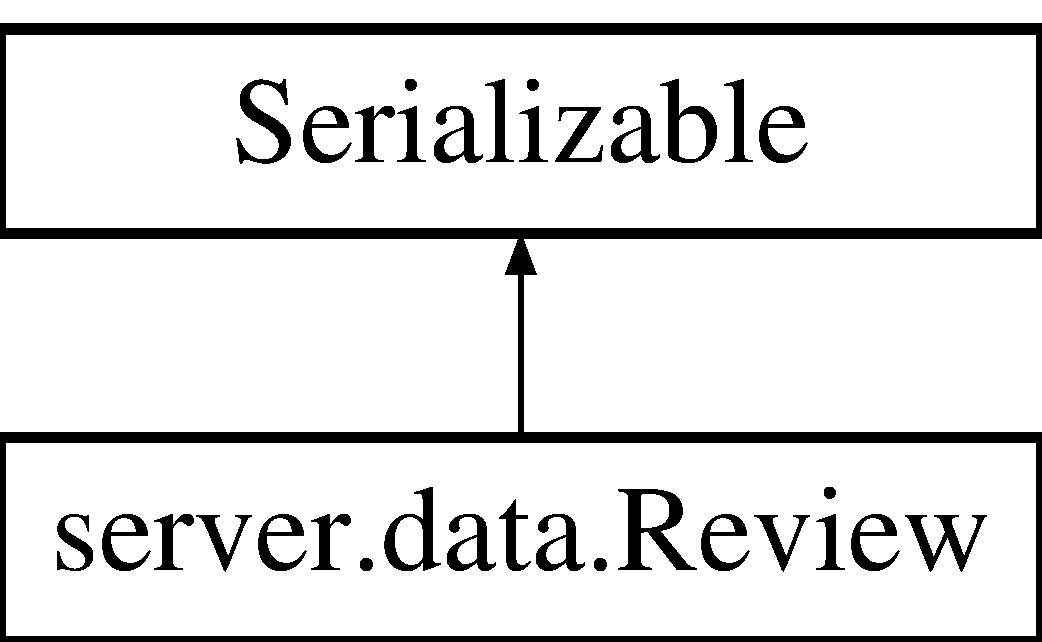
\includegraphics[height=2.000000cm]{classserver_1_1data_1_1_review}
\end{center}
\end{figure}
\subsection*{Public Member Functions}
\begin{DoxyCompactItemize}
\item 
\hyperlink{classserver_1_1data_1_1_review_a4ca7a3db27290b1a96caea6a42e96f36}{Review} (\hyperlink{classserver_1_1data_1_1_user}{User} user, \hyperlink{classserver_1_1data_1_1_book}{Book} book, String comment, double rating)
\item 
\hyperlink{classserver_1_1data_1_1_review_ae9c80d66354aeacd317ad15643580d19}{Review} ()
\item 
\hyperlink{classserver_1_1data_1_1_review_aacee2551f0dcde344e7a7c5d7dc8f30a}{Review} (String comment, double rating)
\item 
\hyperlink{classserver_1_1data_1_1_user}{User} \hyperlink{classserver_1_1data_1_1_review_aae8a51666f66b55a66b4fe7adaba2611}{get\+User} ()
\item 
void \hyperlink{classserver_1_1data_1_1_review_ae3f9c2f431abf254ab7fb35f461fcfe3}{set\+User} (\hyperlink{classserver_1_1data_1_1_user}{User} user)
\item 
\hyperlink{classserver_1_1data_1_1_book}{Book} \hyperlink{classserver_1_1data_1_1_review_a4aca992ed23a4657a326762553cf76e6}{get\+Book} ()
\item 
void \hyperlink{classserver_1_1data_1_1_review_a51000ffda8d748b60488ded30a307bae}{set\+Book} (\hyperlink{classserver_1_1data_1_1_book}{Book} book)
\item 
String \hyperlink{classserver_1_1data_1_1_review_aea59de92d2edb03cf6adf1c3b6c53439}{get\+Comment} ()
\item 
void \hyperlink{classserver_1_1data_1_1_review_a59d8999bf366fdb81b52037a83e8dd15}{set\+Comment} (String comment)
\item 
double \hyperlink{classserver_1_1data_1_1_review_a496eaff532d0bcab68508dc1bda69b54}{get\+Rating} ()
\item 
void \hyperlink{classserver_1_1data_1_1_review_a5a55516c7af44fe0f0b40b1265df333d}{set\+Rating} (double rating)
\item 
int \hyperlink{classserver_1_1data_1_1_review_adc3e4303cb1d78270ae26c30d57c2425}{get\+Id\+\_\+review} ()
\item 
String \hyperlink{classserver_1_1data_1_1_review_a1abc364bd0ad24e6d3d3f33d55a110fc}{to\+String} ()
\item 
void \hyperlink{classserver_1_1data_1_1_review_a7017c3a8ded3a469d06f7866044b1e08}{set\+Id\+\_\+review} (int id\+\_\+review)
\end{DoxyCompactItemize}


\subsection{Constructor \& Destructor Documentation}
\mbox{\Hypertarget{classserver_1_1data_1_1_review_a4ca7a3db27290b1a96caea6a42e96f36}\label{classserver_1_1data_1_1_review_a4ca7a3db27290b1a96caea6a42e96f36}} 
\index{server\+::data\+::\+Review@{server\+::data\+::\+Review}!Review@{Review}}
\index{Review@{Review}!server\+::data\+::\+Review@{server\+::data\+::\+Review}}
\subsubsection{\texorpdfstring{Review()}{Review()}\hspace{0.1cm}{\footnotesize\ttfamily [1/3]}}
{\footnotesize\ttfamily server.\+data.\+Review.\+Review (\begin{DoxyParamCaption}\item[{\hyperlink{classserver_1_1data_1_1_user}{User}}]{user,  }\item[{\hyperlink{classserver_1_1data_1_1_book}{Book}}]{book,  }\item[{String}]{comment,  }\item[{double}]{rating }\end{DoxyParamCaption})}

\mbox{\Hypertarget{classserver_1_1data_1_1_review_ae9c80d66354aeacd317ad15643580d19}\label{classserver_1_1data_1_1_review_ae9c80d66354aeacd317ad15643580d19}} 
\index{server\+::data\+::\+Review@{server\+::data\+::\+Review}!Review@{Review}}
\index{Review@{Review}!server\+::data\+::\+Review@{server\+::data\+::\+Review}}
\subsubsection{\texorpdfstring{Review()}{Review()}\hspace{0.1cm}{\footnotesize\ttfamily [2/3]}}
{\footnotesize\ttfamily server.\+data.\+Review.\+Review (\begin{DoxyParamCaption}{ }\end{DoxyParamCaption})}

\mbox{\Hypertarget{classserver_1_1data_1_1_review_aacee2551f0dcde344e7a7c5d7dc8f30a}\label{classserver_1_1data_1_1_review_aacee2551f0dcde344e7a7c5d7dc8f30a}} 
\index{server\+::data\+::\+Review@{server\+::data\+::\+Review}!Review@{Review}}
\index{Review@{Review}!server\+::data\+::\+Review@{server\+::data\+::\+Review}}
\subsubsection{\texorpdfstring{Review()}{Review()}\hspace{0.1cm}{\footnotesize\ttfamily [3/3]}}
{\footnotesize\ttfamily server.\+data.\+Review.\+Review (\begin{DoxyParamCaption}\item[{String}]{comment,  }\item[{double}]{rating }\end{DoxyParamCaption})}



\subsection{Member Function Documentation}
\mbox{\Hypertarget{classserver_1_1data_1_1_review_a4aca992ed23a4657a326762553cf76e6}\label{classserver_1_1data_1_1_review_a4aca992ed23a4657a326762553cf76e6}} 
\index{server\+::data\+::\+Review@{server\+::data\+::\+Review}!get\+Book@{get\+Book}}
\index{get\+Book@{get\+Book}!server\+::data\+::\+Review@{server\+::data\+::\+Review}}
\subsubsection{\texorpdfstring{get\+Book()}{getBook()}}
{\footnotesize\ttfamily \hyperlink{classserver_1_1data_1_1_book}{Book} server.\+data.\+Review.\+get\+Book (\begin{DoxyParamCaption}{ }\end{DoxyParamCaption})}

\mbox{\Hypertarget{classserver_1_1data_1_1_review_aea59de92d2edb03cf6adf1c3b6c53439}\label{classserver_1_1data_1_1_review_aea59de92d2edb03cf6adf1c3b6c53439}} 
\index{server\+::data\+::\+Review@{server\+::data\+::\+Review}!get\+Comment@{get\+Comment}}
\index{get\+Comment@{get\+Comment}!server\+::data\+::\+Review@{server\+::data\+::\+Review}}
\subsubsection{\texorpdfstring{get\+Comment()}{getComment()}}
{\footnotesize\ttfamily String server.\+data.\+Review.\+get\+Comment (\begin{DoxyParamCaption}{ }\end{DoxyParamCaption})}

\mbox{\Hypertarget{classserver_1_1data_1_1_review_adc3e4303cb1d78270ae26c30d57c2425}\label{classserver_1_1data_1_1_review_adc3e4303cb1d78270ae26c30d57c2425}} 
\index{server\+::data\+::\+Review@{server\+::data\+::\+Review}!get\+Id\+\_\+review@{get\+Id\+\_\+review}}
\index{get\+Id\+\_\+review@{get\+Id\+\_\+review}!server\+::data\+::\+Review@{server\+::data\+::\+Review}}
\subsubsection{\texorpdfstring{get\+Id\+\_\+review()}{getId\_review()}}
{\footnotesize\ttfamily int server.\+data.\+Review.\+get\+Id\+\_\+review (\begin{DoxyParamCaption}{ }\end{DoxyParamCaption})}

\mbox{\Hypertarget{classserver_1_1data_1_1_review_a496eaff532d0bcab68508dc1bda69b54}\label{classserver_1_1data_1_1_review_a496eaff532d0bcab68508dc1bda69b54}} 
\index{server\+::data\+::\+Review@{server\+::data\+::\+Review}!get\+Rating@{get\+Rating}}
\index{get\+Rating@{get\+Rating}!server\+::data\+::\+Review@{server\+::data\+::\+Review}}
\subsubsection{\texorpdfstring{get\+Rating()}{getRating()}}
{\footnotesize\ttfamily double server.\+data.\+Review.\+get\+Rating (\begin{DoxyParamCaption}{ }\end{DoxyParamCaption})}

\mbox{\Hypertarget{classserver_1_1data_1_1_review_aae8a51666f66b55a66b4fe7adaba2611}\label{classserver_1_1data_1_1_review_aae8a51666f66b55a66b4fe7adaba2611}} 
\index{server\+::data\+::\+Review@{server\+::data\+::\+Review}!get\+User@{get\+User}}
\index{get\+User@{get\+User}!server\+::data\+::\+Review@{server\+::data\+::\+Review}}
\subsubsection{\texorpdfstring{get\+User()}{getUser()}}
{\footnotesize\ttfamily \hyperlink{classserver_1_1data_1_1_user}{User} server.\+data.\+Review.\+get\+User (\begin{DoxyParamCaption}{ }\end{DoxyParamCaption})}

\mbox{\Hypertarget{classserver_1_1data_1_1_review_a51000ffda8d748b60488ded30a307bae}\label{classserver_1_1data_1_1_review_a51000ffda8d748b60488ded30a307bae}} 
\index{server\+::data\+::\+Review@{server\+::data\+::\+Review}!set\+Book@{set\+Book}}
\index{set\+Book@{set\+Book}!server\+::data\+::\+Review@{server\+::data\+::\+Review}}
\subsubsection{\texorpdfstring{set\+Book()}{setBook()}}
{\footnotesize\ttfamily void server.\+data.\+Review.\+set\+Book (\begin{DoxyParamCaption}\item[{\hyperlink{classserver_1_1data_1_1_book}{Book}}]{book }\end{DoxyParamCaption})}

\mbox{\Hypertarget{classserver_1_1data_1_1_review_a59d8999bf366fdb81b52037a83e8dd15}\label{classserver_1_1data_1_1_review_a59d8999bf366fdb81b52037a83e8dd15}} 
\index{server\+::data\+::\+Review@{server\+::data\+::\+Review}!set\+Comment@{set\+Comment}}
\index{set\+Comment@{set\+Comment}!server\+::data\+::\+Review@{server\+::data\+::\+Review}}
\subsubsection{\texorpdfstring{set\+Comment()}{setComment()}}
{\footnotesize\ttfamily void server.\+data.\+Review.\+set\+Comment (\begin{DoxyParamCaption}\item[{String}]{comment }\end{DoxyParamCaption})}

\mbox{\Hypertarget{classserver_1_1data_1_1_review_a7017c3a8ded3a469d06f7866044b1e08}\label{classserver_1_1data_1_1_review_a7017c3a8ded3a469d06f7866044b1e08}} 
\index{server\+::data\+::\+Review@{server\+::data\+::\+Review}!set\+Id\+\_\+review@{set\+Id\+\_\+review}}
\index{set\+Id\+\_\+review@{set\+Id\+\_\+review}!server\+::data\+::\+Review@{server\+::data\+::\+Review}}
\subsubsection{\texorpdfstring{set\+Id\+\_\+review()}{setId\_review()}}
{\footnotesize\ttfamily void server.\+data.\+Review.\+set\+Id\+\_\+review (\begin{DoxyParamCaption}\item[{int}]{id\+\_\+review }\end{DoxyParamCaption})}

\mbox{\Hypertarget{classserver_1_1data_1_1_review_a5a55516c7af44fe0f0b40b1265df333d}\label{classserver_1_1data_1_1_review_a5a55516c7af44fe0f0b40b1265df333d}} 
\index{server\+::data\+::\+Review@{server\+::data\+::\+Review}!set\+Rating@{set\+Rating}}
\index{set\+Rating@{set\+Rating}!server\+::data\+::\+Review@{server\+::data\+::\+Review}}
\subsubsection{\texorpdfstring{set\+Rating()}{setRating()}}
{\footnotesize\ttfamily void server.\+data.\+Review.\+set\+Rating (\begin{DoxyParamCaption}\item[{double}]{rating }\end{DoxyParamCaption})}

\mbox{\Hypertarget{classserver_1_1data_1_1_review_ae3f9c2f431abf254ab7fb35f461fcfe3}\label{classserver_1_1data_1_1_review_ae3f9c2f431abf254ab7fb35f461fcfe3}} 
\index{server\+::data\+::\+Review@{server\+::data\+::\+Review}!set\+User@{set\+User}}
\index{set\+User@{set\+User}!server\+::data\+::\+Review@{server\+::data\+::\+Review}}
\subsubsection{\texorpdfstring{set\+User()}{setUser()}}
{\footnotesize\ttfamily void server.\+data.\+Review.\+set\+User (\begin{DoxyParamCaption}\item[{\hyperlink{classserver_1_1data_1_1_user}{User}}]{user }\end{DoxyParamCaption})}

\mbox{\Hypertarget{classserver_1_1data_1_1_review_a1abc364bd0ad24e6d3d3f33d55a110fc}\label{classserver_1_1data_1_1_review_a1abc364bd0ad24e6d3d3f33d55a110fc}} 
\index{server\+::data\+::\+Review@{server\+::data\+::\+Review}!to\+String@{to\+String}}
\index{to\+String@{to\+String}!server\+::data\+::\+Review@{server\+::data\+::\+Review}}
\subsubsection{\texorpdfstring{to\+String()}{toString()}}
{\footnotesize\ttfamily String server.\+data.\+Review.\+to\+String (\begin{DoxyParamCaption}{ }\end{DoxyParamCaption})}



The documentation for this class was generated from the following file\+:\begin{DoxyCompactItemize}
\item 
src/main/java/server/data/\hyperlink{_review_8java}{Review.\+java}\end{DoxyCompactItemize}

\hypertarget{classserver_1_1_r_m_i_test}{}\section{server.\+R\+M\+I\+Test Class Reference}
\label{classserver_1_1_r_m_i_test}\index{server.\+R\+M\+I\+Test@{server.\+R\+M\+I\+Test}}
\subsection*{Public Member Functions}
\begin{DoxyCompactItemize}
\item 
void \hyperlink{classserver_1_1_r_m_i_test_afa84bf10a728f823fac69db153b1c3e7}{set\+Up\+Client} ()
\item 
void \hyperlink{classserver_1_1_r_m_i_test_ac9e55699ef63db0bf72493ced80157fb}{register\+New\+User\+Test} ()
\item 
void \hyperlink{classserver_1_1_r_m_i_test_a7553f5b5e7d2b250abfd675bd5cb9428}{register\+Existing\+User\+Test} ()
\item 
void \hyperlink{classserver_1_1_r_m_i_test_a97c45d5c0c201e134f55458289f1a189}{book\+Test\+Validation} ()
\item 
void \hyperlink{classserver_1_1_r_m_i_test_a9229c65573d1e487439fa0deacde9d35}{show\+Books\+In\+Store\+Test} ()
\item 
void \hyperlink{classserver_1_1_r_m_i_test_a47e723272e2b510190efc5342d478757}{show\+Users\+Test} ()
\item 
void \hyperlink{classserver_1_1_r_m_i_test_abde374312c6ab45dfac4abf722472910}{get\+Things} ()
\item 
void \hyperlink{classserver_1_1_r_m_i_test_a9e1541bcb7b6629caf2462f1d89b164e}{show\+User\+Fail\+Test} ()  throws Remote\+Exception
\end{DoxyCompactItemize}
\subsection*{Static Public Member Functions}
\begin{DoxyCompactItemize}
\item 
static junit.\+framework.\+Test \hyperlink{classserver_1_1_r_m_i_test_a66cf8d2b5563f466516d5d5addd874df}{suite} ()
\item 
static void \hyperlink{classserver_1_1_r_m_i_test_a9b395f99eaaa51d877c3a505294e0fe8}{set\+Up} ()
\item 
static void \hyperlink{classserver_1_1_r_m_i_test_af542aed2dc3097307cfc2e0b5bec3c95}{tear\+Down} ()
\end{DoxyCompactItemize}


\subsection{Detailed Description}
R\+MI Unit test for Simple Client / \hyperlink{classserver_1_1_server}{Server} R\+MI Testing. Testing the only the Remoteness 

\subsection{Member Function Documentation}
\mbox{\Hypertarget{classserver_1_1_r_m_i_test_a97c45d5c0c201e134f55458289f1a189}\label{classserver_1_1_r_m_i_test_a97c45d5c0c201e134f55458289f1a189}} 
\index{server\+::\+R\+M\+I\+Test@{server\+::\+R\+M\+I\+Test}!book\+Test\+Validation@{book\+Test\+Validation}}
\index{book\+Test\+Validation@{book\+Test\+Validation}!server\+::\+R\+M\+I\+Test@{server\+::\+R\+M\+I\+Test}}
\subsubsection{\texorpdfstring{book\+Test\+Validation()}{bookTestValidation()}}
{\footnotesize\ttfamily void server.\+R\+M\+I\+Test.\+book\+Test\+Validation (\begin{DoxyParamCaption}{ }\end{DoxyParamCaption})}

\mbox{\Hypertarget{classserver_1_1_r_m_i_test_abde374312c6ab45dfac4abf722472910}\label{classserver_1_1_r_m_i_test_abde374312c6ab45dfac4abf722472910}} 
\index{server\+::\+R\+M\+I\+Test@{server\+::\+R\+M\+I\+Test}!get\+Things@{get\+Things}}
\index{get\+Things@{get\+Things}!server\+::\+R\+M\+I\+Test@{server\+::\+R\+M\+I\+Test}}
\subsubsection{\texorpdfstring{get\+Things()}{getThings()}}
{\footnotesize\ttfamily void server.\+R\+M\+I\+Test.\+get\+Things (\begin{DoxyParamCaption}{ }\end{DoxyParamCaption})}

\mbox{\Hypertarget{classserver_1_1_r_m_i_test_a7553f5b5e7d2b250abfd675bd5cb9428}\label{classserver_1_1_r_m_i_test_a7553f5b5e7d2b250abfd675bd5cb9428}} 
\index{server\+::\+R\+M\+I\+Test@{server\+::\+R\+M\+I\+Test}!register\+Existing\+User\+Test@{register\+Existing\+User\+Test}}
\index{register\+Existing\+User\+Test@{register\+Existing\+User\+Test}!server\+::\+R\+M\+I\+Test@{server\+::\+R\+M\+I\+Test}}
\subsubsection{\texorpdfstring{register\+Existing\+User\+Test()}{registerExistingUserTest()}}
{\footnotesize\ttfamily void server.\+R\+M\+I\+Test.\+register\+Existing\+User\+Test (\begin{DoxyParamCaption}{ }\end{DoxyParamCaption})}

\mbox{\Hypertarget{classserver_1_1_r_m_i_test_ac9e55699ef63db0bf72493ced80157fb}\label{classserver_1_1_r_m_i_test_ac9e55699ef63db0bf72493ced80157fb}} 
\index{server\+::\+R\+M\+I\+Test@{server\+::\+R\+M\+I\+Test}!register\+New\+User\+Test@{register\+New\+User\+Test}}
\index{register\+New\+User\+Test@{register\+New\+User\+Test}!server\+::\+R\+M\+I\+Test@{server\+::\+R\+M\+I\+Test}}
\subsubsection{\texorpdfstring{register\+New\+User\+Test()}{registerNewUserTest()}}
{\footnotesize\ttfamily void server.\+R\+M\+I\+Test.\+register\+New\+User\+Test (\begin{DoxyParamCaption}{ }\end{DoxyParamCaption})}

\mbox{\Hypertarget{classserver_1_1_r_m_i_test_a9b395f99eaaa51d877c3a505294e0fe8}\label{classserver_1_1_r_m_i_test_a9b395f99eaaa51d877c3a505294e0fe8}} 
\index{server\+::\+R\+M\+I\+Test@{server\+::\+R\+M\+I\+Test}!set\+Up@{set\+Up}}
\index{set\+Up@{set\+Up}!server\+::\+R\+M\+I\+Test@{server\+::\+R\+M\+I\+Test}}
\subsubsection{\texorpdfstring{set\+Up()}{setUp()}}
{\footnotesize\ttfamily static void server.\+R\+M\+I\+Test.\+set\+Up (\begin{DoxyParamCaption}{ }\end{DoxyParamCaption})\hspace{0.3cm}{\ttfamily [static]}}

\mbox{\Hypertarget{classserver_1_1_r_m_i_test_afa84bf10a728f823fac69db153b1c3e7}\label{classserver_1_1_r_m_i_test_afa84bf10a728f823fac69db153b1c3e7}} 
\index{server\+::\+R\+M\+I\+Test@{server\+::\+R\+M\+I\+Test}!set\+Up\+Client@{set\+Up\+Client}}
\index{set\+Up\+Client@{set\+Up\+Client}!server\+::\+R\+M\+I\+Test@{server\+::\+R\+M\+I\+Test}}
\subsubsection{\texorpdfstring{set\+Up\+Client()}{setUpClient()}}
{\footnotesize\ttfamily void server.\+R\+M\+I\+Test.\+set\+Up\+Client (\begin{DoxyParamCaption}{ }\end{DoxyParamCaption})}

\mbox{\Hypertarget{classserver_1_1_r_m_i_test_a9229c65573d1e487439fa0deacde9d35}\label{classserver_1_1_r_m_i_test_a9229c65573d1e487439fa0deacde9d35}} 
\index{server\+::\+R\+M\+I\+Test@{server\+::\+R\+M\+I\+Test}!show\+Books\+In\+Store\+Test@{show\+Books\+In\+Store\+Test}}
\index{show\+Books\+In\+Store\+Test@{show\+Books\+In\+Store\+Test}!server\+::\+R\+M\+I\+Test@{server\+::\+R\+M\+I\+Test}}
\subsubsection{\texorpdfstring{show\+Books\+In\+Store\+Test()}{showBooksInStoreTest()}}
{\footnotesize\ttfamily void server.\+R\+M\+I\+Test.\+show\+Books\+In\+Store\+Test (\begin{DoxyParamCaption}{ }\end{DoxyParamCaption})}

\mbox{\Hypertarget{classserver_1_1_r_m_i_test_a9e1541bcb7b6629caf2462f1d89b164e}\label{classserver_1_1_r_m_i_test_a9e1541bcb7b6629caf2462f1d89b164e}} 
\index{server\+::\+R\+M\+I\+Test@{server\+::\+R\+M\+I\+Test}!show\+User\+Fail\+Test@{show\+User\+Fail\+Test}}
\index{show\+User\+Fail\+Test@{show\+User\+Fail\+Test}!server\+::\+R\+M\+I\+Test@{server\+::\+R\+M\+I\+Test}}
\subsubsection{\texorpdfstring{show\+User\+Fail\+Test()}{showUserFailTest()}}
{\footnotesize\ttfamily void server.\+R\+M\+I\+Test.\+show\+User\+Fail\+Test (\begin{DoxyParamCaption}{ }\end{DoxyParamCaption}) throws Remote\+Exception}

\mbox{\Hypertarget{classserver_1_1_r_m_i_test_a47e723272e2b510190efc5342d478757}\label{classserver_1_1_r_m_i_test_a47e723272e2b510190efc5342d478757}} 
\index{server\+::\+R\+M\+I\+Test@{server\+::\+R\+M\+I\+Test}!show\+Users\+Test@{show\+Users\+Test}}
\index{show\+Users\+Test@{show\+Users\+Test}!server\+::\+R\+M\+I\+Test@{server\+::\+R\+M\+I\+Test}}
\subsubsection{\texorpdfstring{show\+Users\+Test()}{showUsersTest()}}
{\footnotesize\ttfamily void server.\+R\+M\+I\+Test.\+show\+Users\+Test (\begin{DoxyParamCaption}{ }\end{DoxyParamCaption})}

\mbox{\Hypertarget{classserver_1_1_r_m_i_test_a66cf8d2b5563f466516d5d5addd874df}\label{classserver_1_1_r_m_i_test_a66cf8d2b5563f466516d5d5addd874df}} 
\index{server\+::\+R\+M\+I\+Test@{server\+::\+R\+M\+I\+Test}!suite@{suite}}
\index{suite@{suite}!server\+::\+R\+M\+I\+Test@{server\+::\+R\+M\+I\+Test}}
\subsubsection{\texorpdfstring{suite()}{suite()}}
{\footnotesize\ttfamily static junit.\+framework.\+Test server.\+R\+M\+I\+Test.\+suite (\begin{DoxyParamCaption}{ }\end{DoxyParamCaption})\hspace{0.3cm}{\ttfamily [static]}}

\mbox{\Hypertarget{classserver_1_1_r_m_i_test_af542aed2dc3097307cfc2e0b5bec3c95}\label{classserver_1_1_r_m_i_test_af542aed2dc3097307cfc2e0b5bec3c95}} 
\index{server\+::\+R\+M\+I\+Test@{server\+::\+R\+M\+I\+Test}!tear\+Down@{tear\+Down}}
\index{tear\+Down@{tear\+Down}!server\+::\+R\+M\+I\+Test@{server\+::\+R\+M\+I\+Test}}
\subsubsection{\texorpdfstring{tear\+Down()}{tearDown()}}
{\footnotesize\ttfamily static void server.\+R\+M\+I\+Test.\+tear\+Down (\begin{DoxyParamCaption}{ }\end{DoxyParamCaption})\hspace{0.3cm}{\ttfamily [static]}}

public void delete\+Database() \{ Persistence\+Manager\+Factory pmf = J\+D\+O\+Helper.\+get\+Persistence\+Manager\+Factory(\char`\"{}datanucleus.\+properties\char`\"{}); Persistence\+Manager pm = pmf.\+get\+Persistence\+Manager(); Transaction tx = pm.\+current\+Transaction(); try \{ tx.\+begin();

logger.\+info(\char`\"{}\+Deleting test users from persistence. Cleaning up.\char`\"{}); Query$<$\+User$>$ q1 = pm.\+new\+Query(User.\+class); Query$<$\+Book$>$ q2 = pm.\+new\+Query(Book.\+class); Query$<$\+Review$>$ q3 = pm.\+new\+Query(Review.\+class); long number\+Instances\+Deleted1 = q1.\+delete\+Persistent\+All(); long number\+Instances\+Deleted2 = q2.\+delete\+Persistent\+All(); long number\+Instances\+Deleted3 = q3.\+delete\+Persistent\+All();

\begin{DoxyVerb}    tx.commit();
}
finally
{
    if (tx.isActive())
    {
        tx.rollback();
    }
    pm.close();
}
\end{DoxyVerb}


\} 

The documentation for this class was generated from the following file\+:\begin{DoxyCompactItemize}
\item 
src/test/java/server/\hyperlink{_r_m_i_test_8java}{R\+M\+I\+Test.\+java}\end{DoxyCompactItemize}

\hypertarget{classserver_1_1_server}{}\section{server.\+Server Class Reference}
\label{classserver_1_1_server}\index{server.\+Server@{server.\+Server}}
\subsection*{Static Public Member Functions}
\begin{DoxyCompactItemize}
\item 
static void \hyperlink{classserver_1_1_server_acd8e4cb5c187614b7bb0160103e61083}{main} (String\mbox{[}$\,$\mbox{]} args)
\end{DoxyCompactItemize}


\subsection{Member Function Documentation}
\mbox{\Hypertarget{classserver_1_1_server_acd8e4cb5c187614b7bb0160103e61083}\label{classserver_1_1_server_acd8e4cb5c187614b7bb0160103e61083}} 
\index{server\+::\+Server@{server\+::\+Server}!main@{main}}
\index{main@{main}!server\+::\+Server@{server\+::\+Server}}
\subsubsection{\texorpdfstring{main()}{main()}}
{\footnotesize\ttfamily static void server.\+Server.\+main (\begin{DoxyParamCaption}\item[{String \mbox{[}$\,$\mbox{]}}]{args }\end{DoxyParamCaption})\hspace{0.3cm}{\ttfamily [static]}}



The documentation for this class was generated from the following file\+:\begin{DoxyCompactItemize}
\item 
src/main/java/server/\hyperlink{_server_8java}{Server.\+java}\end{DoxyCompactItemize}

\hypertarget{classclient_1_1gui_1_1_show_books}{}\section{client.\+gui.\+Show\+Books Class Reference}
\label{classclient_1_1gui_1_1_show_books}\index{client.\+gui.\+Show\+Books@{client.\+gui.\+Show\+Books}}
\subsection*{Public Member Functions}
\begin{DoxyCompactItemize}
\item 
\hyperlink{classclient_1_1gui_1_1_show_books_a351bf4de3a0981ef4469005bffc1f774}{Show\+Books} (String email)
\end{DoxyCompactItemize}
\subsection*{Static Public Member Functions}
\begin{DoxyCompactItemize}
\item 
static void \hyperlink{classclient_1_1gui_1_1_show_books_acb7c683c6a19a35f85878d376c8b210e}{main} (String\mbox{[}$\,$\mbox{]} args)
\end{DoxyCompactItemize}


\subsection{Constructor \& Destructor Documentation}
\mbox{\Hypertarget{classclient_1_1gui_1_1_show_books_a351bf4de3a0981ef4469005bffc1f774}\label{classclient_1_1gui_1_1_show_books_a351bf4de3a0981ef4469005bffc1f774}} 
\index{client\+::gui\+::\+Show\+Books@{client\+::gui\+::\+Show\+Books}!Show\+Books@{Show\+Books}}
\index{Show\+Books@{Show\+Books}!client\+::gui\+::\+Show\+Books@{client\+::gui\+::\+Show\+Books}}
\subsubsection{\texorpdfstring{Show\+Books()}{ShowBooks()}}
{\footnotesize\ttfamily client.\+gui.\+Show\+Books.\+Show\+Books (\begin{DoxyParamCaption}\item[{String}]{email }\end{DoxyParamCaption})}

Create the application. 

\subsection{Member Function Documentation}
\mbox{\Hypertarget{classclient_1_1gui_1_1_show_books_acb7c683c6a19a35f85878d376c8b210e}\label{classclient_1_1gui_1_1_show_books_acb7c683c6a19a35f85878d376c8b210e}} 
\index{client\+::gui\+::\+Show\+Books@{client\+::gui\+::\+Show\+Books}!main@{main}}
\index{main@{main}!client\+::gui\+::\+Show\+Books@{client\+::gui\+::\+Show\+Books}}
\subsubsection{\texorpdfstring{main()}{main()}}
{\footnotesize\ttfamily static void client.\+gui.\+Show\+Books.\+main (\begin{DoxyParamCaption}\item[{String \mbox{[}$\,$\mbox{]}}]{args }\end{DoxyParamCaption})\hspace{0.3cm}{\ttfamily [static]}}

Launch the application. 

The documentation for this class was generated from the following file\+:\begin{DoxyCompactItemize}
\item 
src/main/java/client/gui/\hyperlink{_show_books_8java}{Show\+Books.\+java}\end{DoxyCompactItemize}

\hypertarget{classclient_1_1gui_1_1_show_description}{}\section{client.\+gui.\+Show\+Description Class Reference}
\label{classclient_1_1gui_1_1_show_description}\index{client.\+gui.\+Show\+Description@{client.\+gui.\+Show\+Description}}
\subsection*{Public Member Functions}
\begin{DoxyCompactItemize}
\item 
\hyperlink{classclient_1_1gui_1_1_show_description_a1c2425fdf8ffa49c58f1757d278243fc}{Show\+Description} (String title, String email, boolean role)  throws Remote\+Exception 
\end{DoxyCompactItemize}


\subsection{Constructor \& Destructor Documentation}
\mbox{\Hypertarget{classclient_1_1gui_1_1_show_description_a1c2425fdf8ffa49c58f1757d278243fc}\label{classclient_1_1gui_1_1_show_description_a1c2425fdf8ffa49c58f1757d278243fc}} 
\index{client\+::gui\+::\+Show\+Description@{client\+::gui\+::\+Show\+Description}!Show\+Description@{Show\+Description}}
\index{Show\+Description@{Show\+Description}!client\+::gui\+::\+Show\+Description@{client\+::gui\+::\+Show\+Description}}
\subsubsection{\texorpdfstring{Show\+Description()}{ShowDescription()}}
{\footnotesize\ttfamily client.\+gui.\+Show\+Description.\+Show\+Description (\begin{DoxyParamCaption}\item[{String}]{title,  }\item[{String}]{email,  }\item[{boolean}]{role }\end{DoxyParamCaption}) throws Remote\+Exception}

Launch the application. Create the application. 
\begin{DoxyParams}{Parameters}
{\em user} & \\
\hline
{\em user} & \\
\hline
\end{DoxyParams}

\begin{DoxyExceptions}{Exceptions}
{\em Remote\+Exception} & \\
\hline
\end{DoxyExceptions}


The documentation for this class was generated from the following file\+:\begin{DoxyCompactItemize}
\item 
src/main/java/client/gui/\hyperlink{_show_description_8java}{Show\+Description.\+java}\end{DoxyCompactItemize}

\hypertarget{classserver_1_1data_1_1_user}{}\section{server.\+data.\+User Class Reference}
\label{classserver_1_1data_1_1_user}\index{server.\+data.\+User@{server.\+data.\+User}}
Inheritance diagram for server.\+data.\+User\+:\begin{figure}[H]
\begin{center}
\leavevmode
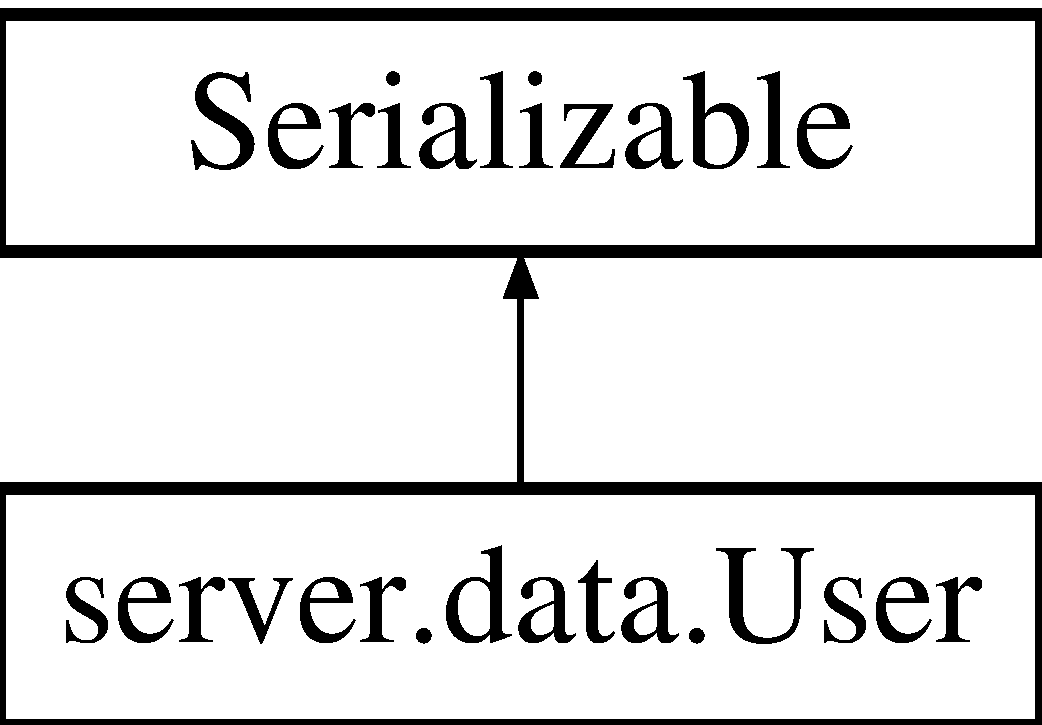
\includegraphics[height=2.000000cm]{classserver_1_1data_1_1_user}
\end{center}
\end{figure}
\subsection*{Public Member Functions}
\begin{DoxyCompactItemize}
\item 
double \hyperlink{classserver_1_1data_1_1_user_a58dcf7faa81b886e169c3b0f074db3d8}{get\+Money} ()
\item 
void \hyperlink{classserver_1_1data_1_1_user_a5448e1a49de3b0057c9bd57b7dcfe888}{set\+Money} (double money)
\item 
\hyperlink{classserver_1_1data_1_1_user_a7167eb7271a1481528efbb6d8f825c76}{User} (String email, String password, String name, String address, boolean role)
\item 
\hyperlink{classserver_1_1data_1_1_user_a43eb15725c3b2bfe218153a48bfbd610}{User} (String email, String password, boolean role)
\item 
void \hyperlink{classserver_1_1data_1_1_user_a5baca76a3ea6ee21979a70c89581fb43}{add\+Review} (\hyperlink{classserver_1_1data_1_1_review}{Review} review)
\item 
void \hyperlink{classserver_1_1data_1_1_user_accc20703f8edd6050d7af19df757925d}{remove\+Review} (\hyperlink{classserver_1_1data_1_1_review}{Review} review)
\item 
List$<$ \hyperlink{classserver_1_1data_1_1_review}{Review} $>$ \hyperlink{classserver_1_1data_1_1_user_aeb59521ec4dddcd7cc91a44ae01e660f}{get\+Reviews} ()
\item 
void \hyperlink{classserver_1_1data_1_1_user_a58385578ceb7c70fc9e8b0d1b2aa2e08}{add\+Book} (\hyperlink{classserver_1_1data_1_1_book}{Book} book)
\item 
void \hyperlink{classserver_1_1data_1_1_user_ab3f96361a26a5281096e526f81f95d7a}{remove\+Book} (\hyperlink{classserver_1_1data_1_1_book}{Book} book)
\item 
List$<$ \hyperlink{classserver_1_1data_1_1_book}{Book} $>$ \hyperlink{classserver_1_1data_1_1_user_aba14990be3bc450a71725f2de9d0eaf0}{get\+Books} ()
\item 
String \hyperlink{classserver_1_1data_1_1_user_ac3981c712bb429f87e43321c10d3858d}{get\+Email} ()
\item 
void \hyperlink{classserver_1_1data_1_1_user_ace8890c975b2543bbbf4d19b4e64d367}{set\+Email} (String email)
\item 
String \hyperlink{classserver_1_1data_1_1_user_af36fc893e682a1b8f79f1e092e7f8057}{get\+Password} ()
\item 
void \hyperlink{classserver_1_1data_1_1_user_a694f243c23ff0620fb683b56f000efc2}{set\+Password} (String password)
\item 
String \hyperlink{classserver_1_1data_1_1_user_ab93c00a3d4afed35078368042d22dcbf}{get\+Name} ()
\item 
void \hyperlink{classserver_1_1data_1_1_user_aab7b2fc87e25728de4b294c9e70811c2}{set\+Name} (String name)
\item 
String \hyperlink{classserver_1_1data_1_1_user_a79d0f524fce79626a9b420b6bb4a8a24}{get\+Address} ()
\item 
void \hyperlink{classserver_1_1data_1_1_user_a7c6d27100b4dbe56de5a9bd4efeb3e13}{set\+Address} (String address)
\item 
boolean \hyperlink{classserver_1_1data_1_1_user_adecb15490622c3c9b813c7c2ebe1616b}{get\+Role} ()
\item 
void \hyperlink{classserver_1_1data_1_1_user_af2ed33ffa1d69585d758713f77b5b079}{set\+Role} (boolean role)
\item 
String \hyperlink{classserver_1_1data_1_1_user_a003500665bb10c335b8d14c1c8fc511e}{to\+String} ()
\end{DoxyCompactItemize}


\subsection{Constructor \& Destructor Documentation}
\mbox{\Hypertarget{classserver_1_1data_1_1_user_a7167eb7271a1481528efbb6d8f825c76}\label{classserver_1_1data_1_1_user_a7167eb7271a1481528efbb6d8f825c76}} 
\index{server\+::data\+::\+User@{server\+::data\+::\+User}!User@{User}}
\index{User@{User}!server\+::data\+::\+User@{server\+::data\+::\+User}}
\subsubsection{\texorpdfstring{User()}{User()}\hspace{0.1cm}{\footnotesize\ttfamily [1/2]}}
{\footnotesize\ttfamily server.\+data.\+User.\+User (\begin{DoxyParamCaption}\item[{String}]{email,  }\item[{String}]{password,  }\item[{String}]{name,  }\item[{String}]{address,  }\item[{boolean}]{role }\end{DoxyParamCaption})}

\mbox{\Hypertarget{classserver_1_1data_1_1_user_a43eb15725c3b2bfe218153a48bfbd610}\label{classserver_1_1data_1_1_user_a43eb15725c3b2bfe218153a48bfbd610}} 
\index{server\+::data\+::\+User@{server\+::data\+::\+User}!User@{User}}
\index{User@{User}!server\+::data\+::\+User@{server\+::data\+::\+User}}
\subsubsection{\texorpdfstring{User()}{User()}\hspace{0.1cm}{\footnotesize\ttfamily [2/2]}}
{\footnotesize\ttfamily server.\+data.\+User.\+User (\begin{DoxyParamCaption}\item[{String}]{email,  }\item[{String}]{password,  }\item[{boolean}]{role }\end{DoxyParamCaption})}



\subsection{Member Function Documentation}
\mbox{\Hypertarget{classserver_1_1data_1_1_user_a58385578ceb7c70fc9e8b0d1b2aa2e08}\label{classserver_1_1data_1_1_user_a58385578ceb7c70fc9e8b0d1b2aa2e08}} 
\index{server\+::data\+::\+User@{server\+::data\+::\+User}!add\+Book@{add\+Book}}
\index{add\+Book@{add\+Book}!server\+::data\+::\+User@{server\+::data\+::\+User}}
\subsubsection{\texorpdfstring{add\+Book()}{addBook()}}
{\footnotesize\ttfamily void server.\+data.\+User.\+add\+Book (\begin{DoxyParamCaption}\item[{\hyperlink{classserver_1_1data_1_1_book}{Book}}]{book }\end{DoxyParamCaption})}

\mbox{\Hypertarget{classserver_1_1data_1_1_user_a5baca76a3ea6ee21979a70c89581fb43}\label{classserver_1_1data_1_1_user_a5baca76a3ea6ee21979a70c89581fb43}} 
\index{server\+::data\+::\+User@{server\+::data\+::\+User}!add\+Review@{add\+Review}}
\index{add\+Review@{add\+Review}!server\+::data\+::\+User@{server\+::data\+::\+User}}
\subsubsection{\texorpdfstring{add\+Review()}{addReview()}}
{\footnotesize\ttfamily void server.\+data.\+User.\+add\+Review (\begin{DoxyParamCaption}\item[{\hyperlink{classserver_1_1data_1_1_review}{Review}}]{review }\end{DoxyParamCaption})}

\mbox{\Hypertarget{classserver_1_1data_1_1_user_a79d0f524fce79626a9b420b6bb4a8a24}\label{classserver_1_1data_1_1_user_a79d0f524fce79626a9b420b6bb4a8a24}} 
\index{server\+::data\+::\+User@{server\+::data\+::\+User}!get\+Address@{get\+Address}}
\index{get\+Address@{get\+Address}!server\+::data\+::\+User@{server\+::data\+::\+User}}
\subsubsection{\texorpdfstring{get\+Address()}{getAddress()}}
{\footnotesize\ttfamily String server.\+data.\+User.\+get\+Address (\begin{DoxyParamCaption}{ }\end{DoxyParamCaption})}

\mbox{\Hypertarget{classserver_1_1data_1_1_user_aba14990be3bc450a71725f2de9d0eaf0}\label{classserver_1_1data_1_1_user_aba14990be3bc450a71725f2de9d0eaf0}} 
\index{server\+::data\+::\+User@{server\+::data\+::\+User}!get\+Books@{get\+Books}}
\index{get\+Books@{get\+Books}!server\+::data\+::\+User@{server\+::data\+::\+User}}
\subsubsection{\texorpdfstring{get\+Books()}{getBooks()}}
{\footnotesize\ttfamily List$<$\hyperlink{classserver_1_1data_1_1_book}{Book}$>$ server.\+data.\+User.\+get\+Books (\begin{DoxyParamCaption}{ }\end{DoxyParamCaption})}

\mbox{\Hypertarget{classserver_1_1data_1_1_user_ac3981c712bb429f87e43321c10d3858d}\label{classserver_1_1data_1_1_user_ac3981c712bb429f87e43321c10d3858d}} 
\index{server\+::data\+::\+User@{server\+::data\+::\+User}!get\+Email@{get\+Email}}
\index{get\+Email@{get\+Email}!server\+::data\+::\+User@{server\+::data\+::\+User}}
\subsubsection{\texorpdfstring{get\+Email()}{getEmail()}}
{\footnotesize\ttfamily String server.\+data.\+User.\+get\+Email (\begin{DoxyParamCaption}{ }\end{DoxyParamCaption})}

\mbox{\Hypertarget{classserver_1_1data_1_1_user_a58dcf7faa81b886e169c3b0f074db3d8}\label{classserver_1_1data_1_1_user_a58dcf7faa81b886e169c3b0f074db3d8}} 
\index{server\+::data\+::\+User@{server\+::data\+::\+User}!get\+Money@{get\+Money}}
\index{get\+Money@{get\+Money}!server\+::data\+::\+User@{server\+::data\+::\+User}}
\subsubsection{\texorpdfstring{get\+Money()}{getMoney()}}
{\footnotesize\ttfamily double server.\+data.\+User.\+get\+Money (\begin{DoxyParamCaption}{ }\end{DoxyParamCaption})}

\mbox{\Hypertarget{classserver_1_1data_1_1_user_ab93c00a3d4afed35078368042d22dcbf}\label{classserver_1_1data_1_1_user_ab93c00a3d4afed35078368042d22dcbf}} 
\index{server\+::data\+::\+User@{server\+::data\+::\+User}!get\+Name@{get\+Name}}
\index{get\+Name@{get\+Name}!server\+::data\+::\+User@{server\+::data\+::\+User}}
\subsubsection{\texorpdfstring{get\+Name()}{getName()}}
{\footnotesize\ttfamily String server.\+data.\+User.\+get\+Name (\begin{DoxyParamCaption}{ }\end{DoxyParamCaption})}

\mbox{\Hypertarget{classserver_1_1data_1_1_user_af36fc893e682a1b8f79f1e092e7f8057}\label{classserver_1_1data_1_1_user_af36fc893e682a1b8f79f1e092e7f8057}} 
\index{server\+::data\+::\+User@{server\+::data\+::\+User}!get\+Password@{get\+Password}}
\index{get\+Password@{get\+Password}!server\+::data\+::\+User@{server\+::data\+::\+User}}
\subsubsection{\texorpdfstring{get\+Password()}{getPassword()}}
{\footnotesize\ttfamily String server.\+data.\+User.\+get\+Password (\begin{DoxyParamCaption}{ }\end{DoxyParamCaption})}

\mbox{\Hypertarget{classserver_1_1data_1_1_user_aeb59521ec4dddcd7cc91a44ae01e660f}\label{classserver_1_1data_1_1_user_aeb59521ec4dddcd7cc91a44ae01e660f}} 
\index{server\+::data\+::\+User@{server\+::data\+::\+User}!get\+Reviews@{get\+Reviews}}
\index{get\+Reviews@{get\+Reviews}!server\+::data\+::\+User@{server\+::data\+::\+User}}
\subsubsection{\texorpdfstring{get\+Reviews()}{getReviews()}}
{\footnotesize\ttfamily List$<$\hyperlink{classserver_1_1data_1_1_review}{Review}$>$ server.\+data.\+User.\+get\+Reviews (\begin{DoxyParamCaption}{ }\end{DoxyParamCaption})}

\mbox{\Hypertarget{classserver_1_1data_1_1_user_adecb15490622c3c9b813c7c2ebe1616b}\label{classserver_1_1data_1_1_user_adecb15490622c3c9b813c7c2ebe1616b}} 
\index{server\+::data\+::\+User@{server\+::data\+::\+User}!get\+Role@{get\+Role}}
\index{get\+Role@{get\+Role}!server\+::data\+::\+User@{server\+::data\+::\+User}}
\subsubsection{\texorpdfstring{get\+Role()}{getRole()}}
{\footnotesize\ttfamily boolean server.\+data.\+User.\+get\+Role (\begin{DoxyParamCaption}{ }\end{DoxyParamCaption})}

\mbox{\Hypertarget{classserver_1_1data_1_1_user_ab3f96361a26a5281096e526f81f95d7a}\label{classserver_1_1data_1_1_user_ab3f96361a26a5281096e526f81f95d7a}} 
\index{server\+::data\+::\+User@{server\+::data\+::\+User}!remove\+Book@{remove\+Book}}
\index{remove\+Book@{remove\+Book}!server\+::data\+::\+User@{server\+::data\+::\+User}}
\subsubsection{\texorpdfstring{remove\+Book()}{removeBook()}}
{\footnotesize\ttfamily void server.\+data.\+User.\+remove\+Book (\begin{DoxyParamCaption}\item[{\hyperlink{classserver_1_1data_1_1_book}{Book}}]{book }\end{DoxyParamCaption})}

\mbox{\Hypertarget{classserver_1_1data_1_1_user_accc20703f8edd6050d7af19df757925d}\label{classserver_1_1data_1_1_user_accc20703f8edd6050d7af19df757925d}} 
\index{server\+::data\+::\+User@{server\+::data\+::\+User}!remove\+Review@{remove\+Review}}
\index{remove\+Review@{remove\+Review}!server\+::data\+::\+User@{server\+::data\+::\+User}}
\subsubsection{\texorpdfstring{remove\+Review()}{removeReview()}}
{\footnotesize\ttfamily void server.\+data.\+User.\+remove\+Review (\begin{DoxyParamCaption}\item[{\hyperlink{classserver_1_1data_1_1_review}{Review}}]{review }\end{DoxyParamCaption})}

\mbox{\Hypertarget{classserver_1_1data_1_1_user_a7c6d27100b4dbe56de5a9bd4efeb3e13}\label{classserver_1_1data_1_1_user_a7c6d27100b4dbe56de5a9bd4efeb3e13}} 
\index{server\+::data\+::\+User@{server\+::data\+::\+User}!set\+Address@{set\+Address}}
\index{set\+Address@{set\+Address}!server\+::data\+::\+User@{server\+::data\+::\+User}}
\subsubsection{\texorpdfstring{set\+Address()}{setAddress()}}
{\footnotesize\ttfamily void server.\+data.\+User.\+set\+Address (\begin{DoxyParamCaption}\item[{String}]{address }\end{DoxyParamCaption})}

\mbox{\Hypertarget{classserver_1_1data_1_1_user_ace8890c975b2543bbbf4d19b4e64d367}\label{classserver_1_1data_1_1_user_ace8890c975b2543bbbf4d19b4e64d367}} 
\index{server\+::data\+::\+User@{server\+::data\+::\+User}!set\+Email@{set\+Email}}
\index{set\+Email@{set\+Email}!server\+::data\+::\+User@{server\+::data\+::\+User}}
\subsubsection{\texorpdfstring{set\+Email()}{setEmail()}}
{\footnotesize\ttfamily void server.\+data.\+User.\+set\+Email (\begin{DoxyParamCaption}\item[{String}]{email }\end{DoxyParamCaption})}

\mbox{\Hypertarget{classserver_1_1data_1_1_user_a5448e1a49de3b0057c9bd57b7dcfe888}\label{classserver_1_1data_1_1_user_a5448e1a49de3b0057c9bd57b7dcfe888}} 
\index{server\+::data\+::\+User@{server\+::data\+::\+User}!set\+Money@{set\+Money}}
\index{set\+Money@{set\+Money}!server\+::data\+::\+User@{server\+::data\+::\+User}}
\subsubsection{\texorpdfstring{set\+Money()}{setMoney()}}
{\footnotesize\ttfamily void server.\+data.\+User.\+set\+Money (\begin{DoxyParamCaption}\item[{double}]{money }\end{DoxyParamCaption})}

\mbox{\Hypertarget{classserver_1_1data_1_1_user_aab7b2fc87e25728de4b294c9e70811c2}\label{classserver_1_1data_1_1_user_aab7b2fc87e25728de4b294c9e70811c2}} 
\index{server\+::data\+::\+User@{server\+::data\+::\+User}!set\+Name@{set\+Name}}
\index{set\+Name@{set\+Name}!server\+::data\+::\+User@{server\+::data\+::\+User}}
\subsubsection{\texorpdfstring{set\+Name()}{setName()}}
{\footnotesize\ttfamily void server.\+data.\+User.\+set\+Name (\begin{DoxyParamCaption}\item[{String}]{name }\end{DoxyParamCaption})}

\mbox{\Hypertarget{classserver_1_1data_1_1_user_a694f243c23ff0620fb683b56f000efc2}\label{classserver_1_1data_1_1_user_a694f243c23ff0620fb683b56f000efc2}} 
\index{server\+::data\+::\+User@{server\+::data\+::\+User}!set\+Password@{set\+Password}}
\index{set\+Password@{set\+Password}!server\+::data\+::\+User@{server\+::data\+::\+User}}
\subsubsection{\texorpdfstring{set\+Password()}{setPassword()}}
{\footnotesize\ttfamily void server.\+data.\+User.\+set\+Password (\begin{DoxyParamCaption}\item[{String}]{password }\end{DoxyParamCaption})}

\mbox{\Hypertarget{classserver_1_1data_1_1_user_af2ed33ffa1d69585d758713f77b5b079}\label{classserver_1_1data_1_1_user_af2ed33ffa1d69585d758713f77b5b079}} 
\index{server\+::data\+::\+User@{server\+::data\+::\+User}!set\+Role@{set\+Role}}
\index{set\+Role@{set\+Role}!server\+::data\+::\+User@{server\+::data\+::\+User}}
\subsubsection{\texorpdfstring{set\+Role()}{setRole()}}
{\footnotesize\ttfamily void server.\+data.\+User.\+set\+Role (\begin{DoxyParamCaption}\item[{boolean}]{role }\end{DoxyParamCaption})}

\mbox{\Hypertarget{classserver_1_1data_1_1_user_a003500665bb10c335b8d14c1c8fc511e}\label{classserver_1_1data_1_1_user_a003500665bb10c335b8d14c1c8fc511e}} 
\index{server\+::data\+::\+User@{server\+::data\+::\+User}!to\+String@{to\+String}}
\index{to\+String@{to\+String}!server\+::data\+::\+User@{server\+::data\+::\+User}}
\subsubsection{\texorpdfstring{to\+String()}{toString()}}
{\footnotesize\ttfamily String server.\+data.\+User.\+to\+String (\begin{DoxyParamCaption}{ }\end{DoxyParamCaption})}



The documentation for this class was generated from the following file\+:\begin{DoxyCompactItemize}
\item 
src/main/java/server/data/\hyperlink{_user_8java}{User.\+java}\end{DoxyCompactItemize}

\chapter{File Documentation}
\hypertarget{_client_8java}{}\section{src/main/java/client/\+Client.java File Reference}
\label{_client_8java}\index{src/main/java/client/\+Client.\+java@{src/main/java/client/\+Client.\+java}}
\subsection*{Classes}
\begin{DoxyCompactItemize}
\item 
class \hyperlink{classclient_1_1_client}{client.\+Client}
\end{DoxyCompactItemize}
\subsection*{Packages}
\begin{DoxyCompactItemize}
\item 
package \hyperlink{namespaceclient}{client}
\end{DoxyCompactItemize}

\hypertarget{_log_in_8java}{}\section{src/main/java/client/gui/\+Log\+In.java File Reference}
\label{_log_in_8java}\index{src/main/java/client/gui/\+Log\+In.\+java@{src/main/java/client/gui/\+Log\+In.\+java}}
\subsection*{Classes}
\begin{DoxyCompactItemize}
\item 
class \hyperlink{classclient_1_1gui_1_1_log_in}{client.\+gui.\+Log\+In}
\end{DoxyCompactItemize}
\subsection*{Packages}
\begin{DoxyCompactItemize}
\item 
package \hyperlink{namespaceclient_1_1gui}{client.\+gui}
\end{DoxyCompactItemize}

\hypertarget{_show_books_8java}{}\section{src/main/java/client/gui/\+Show\+Books.java File Reference}
\label{_show_books_8java}\index{src/main/java/client/gui/\+Show\+Books.\+java@{src/main/java/client/gui/\+Show\+Books.\+java}}
\subsection*{Classes}
\begin{DoxyCompactItemize}
\item 
class \hyperlink{classclient_1_1gui_1_1_show_books}{client.\+gui.\+Show\+Books}
\item 
class {\bfseries client.\+gui.\+Book\+Table\+Model}
\end{DoxyCompactItemize}
\subsection*{Packages}
\begin{DoxyCompactItemize}
\item 
package \hyperlink{namespaceclient_1_1gui}{client.\+gui}
\end{DoxyCompactItemize}

\hypertarget{_show_description_8java}{}\section{src/main/java/client/gui/\+Show\+Description.java File Reference}
\label{_show_description_8java}\index{src/main/java/client/gui/\+Show\+Description.\+java@{src/main/java/client/gui/\+Show\+Description.\+java}}
\subsection*{Classes}
\begin{DoxyCompactItemize}
\item 
class \hyperlink{classclient_1_1gui_1_1_show_description}{client.\+gui.\+Show\+Description}
\item 
class {\bfseries client.\+gui.\+Review\+Table\+Model}
\end{DoxyCompactItemize}
\subsection*{Packages}
\begin{DoxyCompactItemize}
\item 
package \hyperlink{namespaceclient_1_1gui}{client.\+gui}
\end{DoxyCompactItemize}

\hypertarget{_d_a_o_8java}{}\section{src/main/java/db/\+D\+AO.java File Reference}
\label{_d_a_o_8java}\index{src/main/java/db/\+D\+A\+O.\+java@{src/main/java/db/\+D\+A\+O.\+java}}
\subsection*{Classes}
\begin{DoxyCompactItemize}
\item 
class \hyperlink{classdb_1_1_d_a_o}{db.\+D\+AO}
\end{DoxyCompactItemize}
\subsection*{Packages}
\begin{DoxyCompactItemize}
\item 
package \hyperlink{namespacedb}{db}
\end{DoxyCompactItemize}

\hypertarget{_d_b_8java}{}\section{src/main/java/db/\+DB.java File Reference}
\label{_d_b_8java}\index{src/main/java/db/\+D\+B.\+java@{src/main/java/db/\+D\+B.\+java}}
\subsection*{Classes}
\begin{DoxyCompactItemize}
\item 
class \hyperlink{classdb_1_1_d_b}{db.\+DB}
\end{DoxyCompactItemize}
\subsection*{Packages}
\begin{DoxyCompactItemize}
\item 
package \hyperlink{namespacedb}{db}
\end{DoxyCompactItemize}

\hypertarget{_i_d_a_o_8java}{}\section{src/main/java/db/\+I\+D\+AO.java File Reference}
\label{_i_d_a_o_8java}\index{src/main/java/db/\+I\+D\+A\+O.\+java@{src/main/java/db/\+I\+D\+A\+O.\+java}}
\subsection*{Classes}
\begin{DoxyCompactItemize}
\item 
interface \hyperlink{interfacedb_1_1_i_d_a_o}{db.\+I\+D\+AO}
\end{DoxyCompactItemize}
\subsection*{Packages}
\begin{DoxyCompactItemize}
\item 
package \hyperlink{namespacedb}{db}
\end{DoxyCompactItemize}

\hypertarget{_i_d_b_8java}{}\section{src/main/java/db/\+I\+DB.java File Reference}
\label{_i_d_b_8java}\index{src/main/java/db/\+I\+D\+B.\+java@{src/main/java/db/\+I\+D\+B.\+java}}
\subsection*{Classes}
\begin{DoxyCompactItemize}
\item 
interface \hyperlink{interfacedb_1_1_i_d_b}{db.\+I\+DB}
\end{DoxyCompactItemize}
\subsection*{Packages}
\begin{DoxyCompactItemize}
\item 
package \hyperlink{namespacedb}{db}
\end{DoxyCompactItemize}

\hypertarget{_book_8java}{}\section{src/main/java/server/data/\+Book.java File Reference}
\label{_book_8java}\index{src/main/java/server/data/\+Book.\+java@{src/main/java/server/data/\+Book.\+java}}
\subsection*{Classes}
\begin{DoxyCompactItemize}
\item 
class \hyperlink{classserver_1_1data_1_1_book}{server.\+data.\+Book}
\end{DoxyCompactItemize}
\subsection*{Packages}
\begin{DoxyCompactItemize}
\item 
package \hyperlink{namespaceserver_1_1data}{server.\+data}
\end{DoxyCompactItemize}

\hypertarget{_review_8java}{}\section{src/main/java/server/data/\+Review.java File Reference}
\label{_review_8java}\index{src/main/java/server/data/\+Review.\+java@{src/main/java/server/data/\+Review.\+java}}
\subsection*{Classes}
\begin{DoxyCompactItemize}
\item 
class \hyperlink{classserver_1_1data_1_1_review}{server.\+data.\+Review}
\end{DoxyCompactItemize}
\subsection*{Packages}
\begin{DoxyCompactItemize}
\item 
package \hyperlink{namespaceserver_1_1data}{server.\+data}
\end{DoxyCompactItemize}

\hypertarget{_user_8java}{}\section{src/main/java/server/data/\+User.java File Reference}
\label{_user_8java}\index{src/main/java/server/data/\+User.\+java@{src/main/java/server/data/\+User.\+java}}
\subsection*{Classes}
\begin{DoxyCompactItemize}
\item 
class \hyperlink{classserver_1_1data_1_1_user}{server.\+data.\+User}
\end{DoxyCompactItemize}
\subsection*{Packages}
\begin{DoxyCompactItemize}
\item 
package \hyperlink{namespaceserver_1_1data}{server.\+data}
\end{DoxyCompactItemize}

\hypertarget{_i_remote_8java}{}\section{src/main/java/server/remote/\+I\+Remote.java File Reference}
\label{_i_remote_8java}\index{src/main/java/server/remote/\+I\+Remote.\+java@{src/main/java/server/remote/\+I\+Remote.\+java}}
\subsection*{Classes}
\begin{DoxyCompactItemize}
\item 
interface \hyperlink{interfaceserver_1_1remote_1_1_i_remote}{server.\+remote.\+I\+Remote}
\end{DoxyCompactItemize}
\subsection*{Packages}
\begin{DoxyCompactItemize}
\item 
package \hyperlink{namespaceserver_1_1remote}{server.\+remote}
\end{DoxyCompactItemize}

\hypertarget{_remote_8java}{}\section{src/main/java/server/remote/\+Remote.java File Reference}
\label{_remote_8java}\index{src/main/java/server/remote/\+Remote.\+java@{src/main/java/server/remote/\+Remote.\+java}}
\subsection*{Classes}
\begin{DoxyCompactItemize}
\item 
class \hyperlink{classserver_1_1remote_1_1_remote}{server.\+remote.\+Remote}
\end{DoxyCompactItemize}
\subsection*{Packages}
\begin{DoxyCompactItemize}
\item 
package \hyperlink{namespaceserver_1_1remote}{server.\+remote}
\end{DoxyCompactItemize}

\hypertarget{_server_8java}{}\section{src/main/java/server/\+Server.java File Reference}
\label{_server_8java}\index{src/main/java/server/\+Server.\+java@{src/main/java/server/\+Server.\+java}}
\subsection*{Classes}
\begin{DoxyCompactItemize}
\item 
class \hyperlink{classserver_1_1_server}{server.\+Server}
\end{DoxyCompactItemize}
\subsection*{Packages}
\begin{DoxyCompactItemize}
\item 
package \hyperlink{namespaceserver}{server}
\end{DoxyCompactItemize}

\hypertarget{_conti_perf_test_8java}{}\section{src/test/java/server/\+Conti\+Perf\+Test.java File Reference}
\label{_conti_perf_test_8java}\index{src/test/java/server/\+Conti\+Perf\+Test.\+java@{src/test/java/server/\+Conti\+Perf\+Test.\+java}}
\subsection*{Classes}
\begin{DoxyCompactItemize}
\item 
class \hyperlink{classserver_1_1_conti_perf_test}{server.\+Conti\+Perf\+Test}
\end{DoxyCompactItemize}
\subsection*{Packages}
\begin{DoxyCompactItemize}
\item 
package \hyperlink{namespaceserver}{server}
\end{DoxyCompactItemize}

\hypertarget{_d_a_o_mock_test_8java}{}\section{src/test/java/server/\+D\+A\+O\+Mock\+Test.java File Reference}
\label{_d_a_o_mock_test_8java}\index{src/test/java/server/\+D\+A\+O\+Mock\+Test.\+java@{src/test/java/server/\+D\+A\+O\+Mock\+Test.\+java}}
\subsection*{Classes}
\begin{DoxyCompactItemize}
\item 
class \hyperlink{classserver_1_1_d_a_o_mock_test}{server.\+D\+A\+O\+Mock\+Test}
\end{DoxyCompactItemize}
\subsection*{Packages}
\begin{DoxyCompactItemize}
\item 
package \hyperlink{namespaceserver}{server}
\end{DoxyCompactItemize}

\hypertarget{_r_m_i_test_8java}{}\section{src/test/java/server/\+R\+M\+I\+Test.java File Reference}
\label{_r_m_i_test_8java}\index{src/test/java/server/\+R\+M\+I\+Test.\+java@{src/test/java/server/\+R\+M\+I\+Test.\+java}}
\subsection*{Classes}
\begin{DoxyCompactItemize}
\item 
class \hyperlink{classserver_1_1_r_m_i_test}{server.\+R\+M\+I\+Test}
\end{DoxyCompactItemize}
\subsection*{Packages}
\begin{DoxyCompactItemize}
\item 
package \hyperlink{namespaceserver}{server}
\end{DoxyCompactItemize}

%--- End generated contents ---

% Index
\backmatter
\newpage
\phantomsection
\clearemptydoublepage
\addcontentsline{toc}{chapter}{Index}
\printindex

\end{document}
